% Configurazione
\documentclass[12pt, a4paper]{report}

\usepackage{graphicx}
\usepackage[table,xcdraw]{xcolor}
%\usepackage{xcolor}
\usepackage{titlesec}
\usepackage{siunitx}
\usepackage{float}
\usepackage{geometry}
\usepackage{fancyhdr}
\usepackage{longtable}
\usepackage[italian]{babel}
\usepackage{longtable}
\usepackage{array}
\newcolumntype{L}[1]{>{\raggedright\arraybackslash}p{#1}}
\newcolumntype{C}[1]{>{\centering\arraybackslash}p{#1}}
\newcolumntype{R}[1]{>{\raggedleft\arraybackslash}p{#1}}

\usepackage{hyperref}
\hypersetup{
    colorlinks,
    linkcolor=black,
    urlcolor=blue
}

\geometry{
  top=30mm,
  bottom=30mm,
  left=30mm,
  right=30mm,
}

\pagestyle{fancy}
\lhead{}
\lfoot{Piano di Progetto}
\cfoot{}
\rfoot{\thepage}
\renewcommand{\headrulewidth}{0.4pt}
\renewcommand{\footrulewidth}{0.4pt}
\setlength{\headheight}{16pt}

\fancypagestyle{firstpage}{%
  \renewcommand{\headrulewidth}{0pt}%
  \renewcommand{\footrulewidth}{0pt}%
  \lfoot{}
  \rfoot{}
}

\graphicspath{ {immagini/} }
\definecolor{RossoUnipd}{HTML}{B5121B}
\titleformat{\chapter}{\normalfont\huge}{\thechapter.}{20pt}{\huge\textbf}

% Variabili
\newcommand{\titolo}{Piano di Progetto}

% Struttura
\begin{document}
  \thispagestyle{firstpage}
  \begin{minipage}[]{0.3\textwidth}
  
\includegraphics[width=0.8\textwidth]{logo_uni}
\end{minipage}
\begin{minipage}[]{0.6\textwidth}
  \textcolor{RossoUnipd}{
    \textbf{Università degli Studi di Padova} \\
    Laurea: Informatica \\
    Corso: Ingegneria del Software \\
    Anno Accademico: 2021/2022
  }
\end{minipage}

\bigskip

\begin{minipage}[]{0.3\textwidth}
  
\includegraphics[width=0.8\textwidth]{logo_merl}
\end{minipage}
\begin{minipage}[]{0.6\textwidth}
  Gruppo: MERL \\
  Email: \texttt{merlunipd@gmail.com}
\end{minipage}

\bigskip
\bigskip
\bigskip

  \begin{center}
  \Huge\textbf{Verbale Riunione}
\end{center}

\begin{center}
  \LARGE\textbf{01 Aprile 2022}
\end{center}

\bigskip
\bigskip
\bigskip

  \newpage
  \begin{center}
  \huge{Registro delle Modifiche}
\end{center}
\renewcommand\arraystretch{1,5}
{\centering
\begin{longtable}{|C{1.8cm}|C{2.1cm}|C{2cm}|C{2.4cm}|L{4.4cm}|}
  \hline
  \rowcolor[HTML]{036400}
  \textcolor[HTML]{FFFFFF}{\textbf{Versione}} & \textcolor[HTML]{FFFFFF}{\textbf{Data}} & \textcolor[HTML]{FFFFFF}{\textbf{Autore}}  & \textcolor[HTML]{FFFFFF}{\textbf{Verificatore}} & \textcolor[HTML]{FFFFFF}{\textbf{Modifica}}    \\ \hline
  \rowcolor[HTML]{EFEFEF}
  v2.0.0        & 04/05/2022    & Mattia Zanellato   &  -  & Approvazione \\ \hline
  \rowcolor[HTML]{C0C0C0}
  v1.0.15       & 04/05/2022    & Mattia Zanellato   &  Marco Mazzucato  & Aggiunta sottosezione "Decimo Periodo" in "Consuntivo" \\ \hline
  \rowcolor[HTML]{EFEFEF}
  v1.0.14       & 27/04/2022    & Emanuele Pase   &   Marco Mazzucato & Aggiunta sottosezione "Decimo Periodo" in "Preventivo" \\ \hline
  \rowcolor[HTML]{C0C0C0}
  v1.0.13       & 26/04/2022    & Riccardo Contin   &  Emanuele Pase  & Aggiunta sottosezione "Nono Periodo" in "Consuntivo" \\ \hline
  \rowcolor[HTML]{EFEFEF}
  v1.0.12       & 21/04/2022    & Riccardo Contin   &  Marco Mazzucato   & Aggiunta sottosezione "Nono Periodo" in "Pianificazione" e in "Preventivo" \\ \hline
  \rowcolor[HTML]{C0C0C0}
  v1.0.11       & 19/04/2022    & Emanuele Pase   &  Marco Mazzucato   & Aggiunta sottosezione "Ottavo Periodo" in "Consuntivo" \\ \hline
  \rowcolor[HTML]{EFEFEF}
  v1.0.10       & 15/04/2022    & Emanuele Pase   &  Marco Mazzucato   & Aggiunta sottosezione "Ottavo Periodo" in "Preventivo" \\ \hline
  \rowcolor[HTML]{C0C0C0}
  v1.0.9        & 13/04/2022    & Marco Mazzucato   &  Riccardo Contin   & Aggiunta sottosezione "Settimo Periodo" in "Consuntivo" \\ \hline
  \rowcolor[HTML]{EFEFEF}
  v1.0.8        & 06/04/2022    & Lorenzo Onelia   &  Riccardo Contin    & Aggiunta sottosezione "Sesto Periodo" in "Consuntivo" \\ \hline
  \rowcolor[HTML]{C0C0C0}
  v1.0.7        & 06/04/2022    & Marco Mazzucato   &   Lorenzo Onelia   & Aggiunta sottosezione "Settimo Periodo" in "Preventivo" \\ \hline
  \rowcolor[HTML]{EFEFEF}
  v1.0.6        & 06/04/2022    & Marco Mazzucato   &  Lorenzo Onelia    & Aggiunta sottosezione "Settimo Periodo" in "Pianificazione" \\ \hline
  \rowcolor[HTML]{C0C0C0}
  v1.0.7        & 31/03/2022    & Lorenzo Onelia   &  Marco Mazzucato    & Aggiunta sottosezione "Sesto Periodo" in "Preventivo" \\ \hline
  \rowcolor[HTML]{EFEFEF}
  v1.0.6        & 31/03/2022    & Lorenzo Onelia   &   Marco Mazzucato   & Aggiunta sottosezione "Sesto Periodo" in "Pianificazione" \\ \hline
  \rowcolor[HTML]{C0C0C0}
  v1.0.5        & 28/03/2022    & Marco Mamprin   &  Marco Mazzucato    & Aggiunta sottosezione "Quinto Periodo" in "Consuntivo" \\ \hline
  \rowcolor[HTML]{EFEFEF}
  v1.0.4        & 27/03/2022    & Marko Vukovic   &  Riccardo Contin    & Aggiunta sottosezione "Semaforo Rosso RTB" in "Consuntivo" \\ \hline
  \rowcolor[HTML]{C0C0C0}
  v1.0.3        & 24/03/2022    & Lorenzo Onelia  & Emanuele Pase    & Fix minori                  \\ \hline
  \rowcolor[HTML]{EFEFEF}
  v1.0.2        & 24/03/2022    & Marco Mamprin   &  Lorenzo Onelia    & Aggiunta sottosezione "Quinto Periodo" in "Preventivo" \\ \hline
  \rowcolor[HTML]{C0C0C0}
  v1.0.1        & 24/03/2022    & Marco Mamprin   &  Lorenzo Onelia    & Aggiunta sottosezione "Quinto Periodo" in "Pianificazione" \\ \hline
  \rowcolor[HTML]{EFEFEF}
  v1.0.0        & 08/03/2022    & Marko Vukovic   &  -                 & Approvazione \\ \hline
  \rowcolor[HTML]{C0C0C0}
  v0.0.17       & 04/03/2022    & Lorenzo Onelia  & Mattia Zanellato     & Aggiunta Lista di distribuzione                  \\ \hline
  \rowcolor[HTML]{EFEFEF}
  v0.0.16       & 24/02/2022     & Riccardo Contin  & Lorenzo Onelia                                & Fix finali \\ \hline
  \rowcolor[HTML]{C0C0C0}
  v0.0.15       & 23/02/2022    & Riccardo Contin   & Lorenzo Onelia                  & Pianificazione futura \\ \hline
  \rowcolor[HTML]{EFEFEF}
  v0.0.14       & 23/02/2022    & Mattia Zanellato  & Marko Vukovic                   & Aggiunta sottosezione "Quarto Periodo" in "Consuntivo" \\ \hline
  \rowcolor[HTML]{C0C0C0}
  v0.0.13       & 17/02/2022    & Riccardo Contin   & Mattia Zanellato                & Modifiche capitolo "Consuntivo" \\ \hline
  \rowcolor[HTML]{EFEFEF}
  v0.0.12       & 16/02/2022    & Mattia Zanellato  & Lorenzo Onelia                  & Aggiunto capitolo "Organigramma" \\ \hline
  \rowcolor[HTML]{C0C0C0}
  v0.0.11       & 11/02/2022    & Mattia Zanellato  & Riccardo Contin                 & Aggiunto capitolo "Mitigazione dei Rischi" \\ \hline
  \rowcolor[HTML]{EFEFEF}
  v0.0.10       & 10/02/2022    & Mattia Zanellato  & Lorenzo Onelia                  & Aggiunto capitolo "Modello di Sviluppo" \\ \hline
  \rowcolor[HTML]{C0C0C0}
  v0.0.9        & 08/02/2022    & Mattia Zanellato  & Lorenzo Onelia                  & Aggiunta sottosezione "Quarto Periodo" in "Preventivo" \\ \hline
  \rowcolor[HTML]{EFEFEF}
  v0.0.8        & 06/02/2022    & Mattia Zanellato  & Lorenzo Onelia                  & Aggiunta sottosezione "Terzo Periodo" in "Consuntivo" \\ \hline
  \rowcolor[HTML]{C0C0C0}
  v0.0.7        & 04/02/2022    & Emanuele Pase     & Marco Mamprin                   & Modifiche capitolo "Pianificazione" \\ \hline
  \rowcolor[HTML]{EFEFEF}
  v0.0.6        & 13/01/2022    & Emanuele Pase     & Marco Mamprin Riccardo Contin   & Aggiunta sottosezione "Secondo Periodo" in "Consuntivo" e sottosezione "Terzo Periodo" in "Preventivo" \\ \hline
  \rowcolor[HTML]{C0C0C0}
  v0.0.5        & 07/01/2022    & Riccardo Contin   & Lorenzo Onelia                  & Aggiunto capitolo "Introduzione" \\ \hline
  \rowcolor[HTML]{EFEFEF}
  v0.0.4        & 28/12/2021    & Riccardo Contin   & Lorenzo Onelia                  & Aggiunta sottosezione "Primo Periodo" in "Consuntivo" e sottosezione "Secondo Periodo" in "Preventivo" \\ \hline
  \rowcolor[HTML]{C0C0C0}
  v0.0.3        & 15/12/2021    & Riccardo Contin   & Marco Mamprin                   & Aggiunta sottosezione "Primo Periodo" in "Preventivo" \\ \hline
  \rowcolor[HTML]{EFEFEF}
  v0.0.2        & 11/12/2021    & Riccardo Contin   & Marco Mamprin                   & Aggiunto capitolo "Analisi dei rischi" \\ \hline
  \rowcolor[HTML]{C0C0C0}
  v0.0.1        & 08/12/2021    & Riccardo Contin   & Marco Mamprin                   & Aggiunto capitolo "Pianificazione" \\ \hline
  \rowcolor[HTML]{EFEFEF}
  v0.0.0        & 07/12/2021    & Riccardo Contin   & Marco Mamprin                   & Creata prima struttura del documento \\ \hline
\end{longtable}}

\renewcommand\arraystretch{1}

  \tableofcontents

  % Capitoli
  \chapter{Introduzione}
\section{Premessa}

Il \textit{Piano di Qualifica} è un documento su cui si prevede di lavorare per l'intera durata del progetto. Molti contenuti di questo documento sono di natura instabile, come alcune metriche che non sono applicabili nella fase iniziale e che solo con il loro utilizzo pratico si può valutarne l'effettiva utilità. Anche i processi selezionati possono essere soggetti a cambiamenti, dato che possono rivelarsi insufficienti o inadeguati agli scopi del progetto e al modo di lavorare del gruppo.
Per tutte queste ragioni il documento è prodotto in maniera incrementale e suoi comntenuti iniziali sono da considerarsi incompleti.

\section{Scopo del documento}
Il \textit{Piano di Qualifica} è un documento che:
\begin{itemize}
    \item Specifica gli obiettivi
    quantitativi di qualità di prodotto e di processo;
    \item Espone le
    metodologie di controllo e le misurazioni di queste qualità tramite
    opportune metriche;
    \item Definisce quanti e quali test eseguire per verificare il corretto funzionamento
    e la qualità dei processi e del prodotto;
    \item Applica questi test e ne documenta l'esito;
    \item Crea un cruscotto di supporto che fornisce
    una visione dello stato corrente degli obiettivi.
\end{itemize}

\section{Scopo del prodotto}
Il capitolato proposto dall'azienda \textit{Zucchetti S.p.A} ha come obiettivo
quello di creare un'applicazione di visualizzazione di dati con numerose dimensioni
che permettono di rintracciare eventuali anomalie attraverso l'occhio umano. Lo
scopo del prodotto è quindi quello di fornire all'utente diversi tipi di
visualizzazione di dati in modo da rendere più veloce ed efficacie l'individuazione
di anomalie.

\section{Glossario}
Per evitare ambiguità relative alle terminoligie utilizzate è stato creato il \textit{Glossario v1.0.0} nel quale sono riportati tutti i termini importanti o con un significato particolare.
\section{Riferimenti}
\subsection{Riferimenti normativi}
\begin{itemize}
  \item \textit{Norme di Progetto v1.0.0}
\end{itemize}
\subsection{Riferimenti informativi}
\begin{itemize}
  \item \textbf{Capitolato d'appalto C5 - Login Warrior}
          \url{https://www.math.unipd.it/~tullio/IS-1/2021/Progetto/C5.pdf}
  \item \textbf{Qualità di processo}
          \url{https://www.math.unipd.it/~tullio/IS-1/2021/Dispense/T13.pdf}
  \item \textbf{Qualità di prodotto}
          \url{https://www.math.unipd.it/~tullio/IS-1/2021/Dispense/T12.pdf}
  \item \textbf{Verifica e validazione}
          \url{https://www.math.unipd.it/~tullio/IS-1/2021/Dispense/T14.pdf}
          \url{https://www.math.unipd.it/~tullio/IS-1/2021/Dispense/T15.pdf}
          \url{https://www.math.unipd.it/~tullio/IS-1/2021/Dispense/T16.pdf}
  \item \textbf{Ciclo di Deming}
          \url{https://it.wikipedia.org/wiki/Ciclo_di_Deming}
  \item \textbf{Indice di Gulpease}
          \url{https://it.wikipedia.org/wiki/Indice_Gulpease}
\end{itemize}

  \chapter{Modello di sviluppo}

\section{Modello agile}
Il gruppo \textit{MERL} ha deciso di ispirarsi ai modelli agili per lo sviluppo del progetto. Questo prevede rilasci multipli e successivi, ciascuno dei quali è in grado di realizzare un incremento di funzionalità.
\\Adottando questo modello risulta necessario individuare e classificare i requisiti$_G$ in modo da poter dare un ordine allo sviluppo che permetterà di ottenere dopo ogni incremento un prodotto, seppur incompleto, stabile e funzionante. Per mantenere questo è fondamentale che i primi incrementi vadano a soddisfare i requisiti più importanti in modo tale da renderli fin da subito stabili all'interno del prodotto. Solo successivamente verranno integrati i requisiti di minor importanza, che avranno dunque più tempo per stabilizzarsi nel prodotto.
\\L'utilizzo dei modelli agili porta in particolare i seguenti vantaggi:
\begin{itemize}
  \item Viene data priorità allo sviluppo delle funzionalità primarie, questo permette una costante verifica$_G$ anche da parte del proponente$_G$ delle principali funzionalità;
  \item Avendo un prodotto funzionante sarà possibile ottenere, dopo ogni incremento, un riscontro da parte del proponente che potrà quindi valutare il funzionamento del prodotto fino a quel momento;
  \item Gli errori saranno facilmente individuabili dato che ogni incremento prevede una fase di verifica finale, questo permette un minor dispendio di risorse per l'individuazione e la risoluzione di tali errori;
  \item La verifica e i test fatti saranno più semplici in quanto saranno volutamente mirati alle modifiche effettuate durante uno specifico incremento;
  \item Permette di rispondere ai cambiamenti in modo molto efficiente, permettendo di rimanere in linea con le aspettative del proponente.
\end{itemize}

  \chapter{Analisi dei rischi}

In un progetto che prevede la realizzazione, da parte di un insieme di persone, di un prodotto concreto 
da consegnare a un proponente è inevitabile che possano verificarsi dei problemi più o meno gravi che
provochino rallentamenti. Per tentare di evitare che accada è necessario fare un'attenta analisi dei
rischi. La nostra aspettativa è quella di riuscire a effettuare delle scelte che ci permettano di
incontrare meno problemi possibili e nel caso se ne verifichi qualcuno avere già pronta una soluzione.

Per organizzare l'analisi ciò che vogliamo evidenziare per ogni rischio è:
\begin{itemize}
    \item Rischio;
    \item Descrizione;
    \item Probabilità di occorrenza;
    \item Grado di pericolosità;
    \item Precauzione;
    \item Piano di contingenza.
\end{itemize}

\newpage
\section{Rischi legati alle persone}


\begin{table}[!ht]
    \renewcommand\arraystretch{1.35}
    \centering
    \begin{tabular}{|ll|}
    \hline
    \rowcolor[HTML]{036400}
    \multicolumn{2}{|c|}{\textcolor{white}{\textbf{Disponibilità}}} \\ \hline
    \rowcolor[HTML]{EFEFEF}\multicolumn{1}{|l|}{\textit{Descrizione}} & \begin{tabular}[c]{@{}l@{}}Ogni membro dovrà affrontare questo progetto sapendo\\ di avere altri impegni universitari e personali.\\ Questo può provocare momenti di inattività o scarsa\\ partecipazione.\end{tabular} \\ \hline
    \rowcolor[HTML]{C0C0C0}\multicolumn{1}{|l|}{\textit{\begin{tabular}[c]{@{}l@{}}Probabilità di\\ occorenza\end{tabular}}} & Alta. \\ \hline
    \rowcolor[HTML]{EFEFEF}\multicolumn{1}{|l|}{\textit{\begin{tabular}[c]{@{}l@{}}Grado di\\ pericolosità\end{tabular}}} & Media. \\ \hline
    \rowcolor[HTML]{C0C0C0}\multicolumn{1}{|l|}{\textit{Precauzioni}} & \begin{tabular}[c]{@{}l@{}}Ogni membro dovrà essere in grado di organizzarsi al\\ meglio in modo da ritagliarsi il tempo necessario alla\\ realizzazione del progetto. Nel caso in cui un membro\\ non abbia nessuna possibilità di operare per un \\ determinato periodo deve avvisare il gruppo.\end{tabular} \\ \hline
    \rowcolor[HTML]{EFEFEF}\multicolumn{1}{|l|}{\textit{\begin{tabular}[c]{@{}l@{}}Piano di\\ contingenza\end{tabular}}} & \begin{tabular}[c]{@{}l@{}}Se la mancanza di uno o più membri sta provocando \\ ritardo, il Responsabile deve ripianificare la suddivisione\\ del lavoro.\end{tabular} \\ \hline
    \end{tabular}
\end{table}

\begin{table}[!ht]
    \renewcommand\arraystretch{1.35}
    \centering
    \begin{tabular}{|ll|}
    \hline
    \rowcolor[HTML]{036400}
    \multicolumn{2}{|c|}{\textcolor{white}{\textbf{Problemi interpersonali}}} \\ \hline
    \rowcolor[HTML]{EFEFEF}\multicolumn{1}{|l|}{\textit{Descrizione}} & \begin{tabular}[c]{@{}l@{}}I gruppi sono stati formati casualmente e per questo\\ è possibile che i membri non si conoscano.\\ C'è il rischio che alcuni membri non vadano \\ molto d'accordo o che non ci sia la massima \\ collaborazione.\end{tabular} \\ \hline
    \rowcolor[HTML]{C0C0C0}\multicolumn{1}{|l|}{\textit{\begin{tabular}[c]{@{}l@{}}Probabilità di\\ occorenza\end{tabular}}} & Bassa. \\ \hline
    \rowcolor[HTML]{EFEFEF}\multicolumn{1}{|l|}{\textit{\begin{tabular}[c]{@{}l@{}}Grado di\\ pericolosità\end{tabular}}} & Alta. \\ \hline
    \rowcolor[HTML]{C0C0C0}\multicolumn{1}{|l|}{\textit{Precauzioni}} & \begin{tabular}[c]{@{}l@{}}Prima di iniziare a lavorare i membri devono imparare a \\ conoscersi ed evitare contrasti ma piuttosto discuterne \\ positivamente.\end{tabular} \\ \hline
    \rowcolor[HTML]{EFEFEF}\multicolumn{1}{|l|}{\textit{\begin{tabular}[c]{@{}l@{}}Piano di\\ contingenza\end{tabular}}} & \begin{tabular}[c]{@{}l@{}}Nel caso si verifichino scontri o ci sia poca collaborazione, \\ il Responsabile deve bloccare il progetto e cercare, \\ con la massima partecipazione di tutti, di risolvere il \\ problema.\end{tabular} \\ \hline
    \end{tabular}
\end{table}

\begin{table}[!ht]
    \renewcommand\arraystretch{1.35}
    \centering
    \begin{tabular}{|ll|}
    \hline
    \rowcolor[HTML]{036400}
    \multicolumn{2}{|c|}{\textcolor{white}{\textbf{Mancanza di esperienza personale}}} \\ \hline
    \rowcolor[HTML]{EFEFEF}\multicolumn{1}{|l|}{\textit{Descrizione}} & \begin{tabular}[c]{@{}l@{}}Data la poca esperienza, ogni membro potrebbe trovarsi\\ in difficoltà durante il progetto.\end{tabular} \\ \hline
    \rowcolor[HTML]{C0C0C0}\multicolumn{1}{|l|}{\textit{\begin{tabular}[c]{@{}l@{}}Probabilità di\\ occorenza\end{tabular}}} & Alta. \\ \hline
    \rowcolor[HTML]{EFEFEF}\multicolumn{1}{|l|}{\textit{\begin{tabular}[c]{@{}l@{}}Grado di\\ pericolosità\end{tabular}}} & Alta. \\ \hline
    \rowcolor[HTML]{C0C0C0}\multicolumn{1}{|l|}{\textit{Precauzioni}} & \begin{tabular}[c]{@{}l@{}}Il gruppo dovrà supportarsi a vicenda cercando di aiutare\\ un membro in difficoltà.\end{tabular} \\ \hline
    \rowcolor[HTML]{EFEFEF}\multicolumn{1}{|l|}{\textit{\begin{tabular}[c]{@{}l@{}}Piano di\\ contingenza\end{tabular}}} & \begin{tabular}[c]{@{}l@{}}Se un membro trova una difficoltà prima di tutto deve\\ tentare di affrontarla, solo successivamente deve chiedere\\ il supporto del Responsabile che si preoccuperà di\\ stabilizzare la situazione.\end{tabular} \\ \hline
    \end{tabular}
\end{table}

\section{Rischi legati all'organizzazione}

\begin{table}[!ht]
    \renewcommand\arraystretch{1.35}
    \centering
    \begin{tabular}{|ll|}
    \hline
    \rowcolor[HTML]{036400}
    \multicolumn{2}{|c|}{\textcolor{white}{\textbf{Scarsa Pianificazione}}} \\ \hline
    \rowcolor[HTML]{EFEFEF}\multicolumn{1}{|l|}{\textit{Descrizione}} & \begin{tabular}[c]{@{}l@{}}Pianificare un intero progetto, individuando le attività e\\ suddividendo i compiti, non è un aspetto facile e questo\\ può provocare ritardi e spreco di risorse.\end{tabular} \\ \hline
    \rowcolor[HTML]{C0C0C0}\multicolumn{1}{|l|}{\textit{\begin{tabular}[c]{@{}l@{}}Probabilità di\\ occorenza\end{tabular}}} & Alta. \\ \hline
    \rowcolor[HTML]{EFEFEF}\multicolumn{1}{|l|}{\textit{\begin{tabular}[c]{@{}l@{}}Grado di\\ pericolosità\end{tabular}}} & Alta. \\ \hline
    \rowcolor[HTML]{C0C0C0}\multicolumn{1}{|l|}{\textit{Precauzioni}} & \begin{tabular}[c]{@{}l@{}}All'inizio la pianificazione deve essere un po'\\ pessimistica ponendo milestones ravvicinate con obiettivi\\ chiari in modo che sia più semplice effettuare correzioni.\end{tabular} \\ \hline
    \rowcolor[HTML]{EFEFEF}\multicolumn{1}{|l|}{\textit{\begin{tabular}[c]{@{}l@{}}Piano di\\ contingenza\end{tabular}}} & \begin{tabular}[c]{@{}l@{}}Se dopo un consuntivo ci si rende conto che la distanza \\ dal preventivo è troppo ampia è necessario ripianificare\\ i periodi successivi prima di fare qualsiasi altra attività.\end{tabular} \\ \hline
    \end{tabular}
\end{table}

\newpage
\section{Rischi legati alle tecnologie e agli strumenti}

\begin{table}[!ht]
    \renewcommand\arraystretch{1.35}
    \centering
    \begin{tabular}{|ll|}
    \hline
    \rowcolor[HTML]{036400}
    \multicolumn{2}{|c|}{\textcolor{white}{\textbf{Strumenti sconosciuti}}} \\ \hline
    \rowcolor[HTML]{EFEFEF}\multicolumn{1}{|l|}{\textit{Descrizione}} & \begin{tabular}[c]{@{}l@{}}A supporto di un buon progetto ci sono degli ottimi\\ strumenti che però non sono immediati da capire e da\\ riuscire ad utilizzare.\end{tabular} \\ \hline
    \rowcolor[HTML]{C0C0C0}\multicolumn{1}{|l|}{\textit{\begin{tabular}[c]{@{}l@{}}Probabilità di\\ occorenza\end{tabular}}} & Media. \\ \hline
    \rowcolor[HTML]{EFEFEF}\multicolumn{1}{|l|}{\textit{\begin{tabular}[c]{@{}l@{}}Grado di\\ pericolosità\end{tabular}}} & Media. \\ \hline
    \rowcolor[HTML]{C0C0C0}\multicolumn{1}{|l|}{\textit{Precauzioni}} & \begin{tabular}[c]{@{}l@{}}Prima di utilizzarne uno, si fa una visione di gruppo\\ dell'utilizzo. Ogni membro poi si preoccuperà di \\ esercitarsi e comprendere tutti gli aspetti utili che lo \\ strumento può offrire senza focalizzarsi troppo su ciò \\ che può risultare inutile.\end{tabular} \\ \hline
    \rowcolor[HTML]{EFEFEF}\multicolumn{1}{|l|}{\textit{\begin{tabular}[c]{@{}l@{}}Piano di\\ contingenza\end{tabular}}} & \begin{tabular}[c]{@{}l@{}}Se l'utilizzo di uno strumento causa ritardi e non è\\ funzionale al progetto, si cerca un alternativa o si\\ valuta di non utilizzarlo direttamente.\end{tabular} \\ \hline
    \end{tabular}
\end{table}

\begin{table}[!ht]
    \renewcommand\arraystretch{1.35}
    \centering
    \begin{tabular}{|ll|}
    \hline
    \rowcolor[HTML]{036400}
    \multicolumn{2}{|c|}{\textcolor{white}{\textbf{Tecnologie sconosciute}}} \\ \hline
    \rowcolor[HTML]{EFEFEF}\multicolumn{1}{|l|}{\textit{Descrizione}} & \begin{tabular}[c]{@{}l@{}}Per la codifica del prodotto software è importante\\ individuare quali siano le tecnologie presenti nel\\ mercato più adatte a ciò che si vuole realizzare. Bisogna\\ però tenere in considerazione che queste possono\\ essere completamente sconosciute ad uno o più membri.\end{tabular} \\ \hline
    \rowcolor[HTML]{C0C0C0}\multicolumn{1}{|l|}{\textit{\begin{tabular}[c]{@{}l@{}}Probabilità di\\ occorenza\end{tabular}}} & Alta. \\ \hline
    \rowcolor[HTML]{EFEFEF}\multicolumn{1}{|l|}{\textit{\begin{tabular}[c]{@{}l@{}}Grado di\\ pericolosità\end{tabular}}} & Alta. \\ \hline
    \rowcolor[HTML]{C0C0C0}\multicolumn{1}{|l|}{\textit{Precauzioni}} & \begin{tabular}[c]{@{}l@{}}Quando si discute di una tecnologia da utilizzare, ogni\\ membro deve esprimere se la conosce e il suo livello.\\ Questo permetterà di capire se la scelta è giusta, ma\\ suggerirà anche la migliore suddivisione del lavoro.\end{tabular} \\ \hline
    \rowcolor[HTML]{EFEFEF}\multicolumn{1}{|l|}{\textit{\begin{tabular}[c]{@{}l@{}}Piano di\\ contingenza\end{tabular}}} & \begin{tabular}[c]{@{}l@{}}Se l'utilizzo di una tecnologia causa ritardi e non è\\ funzionale al progetto, si cerca un alternativa o si punta\\ maggiormente sulla collaborazione per riuscire a trovare\\ una soluzione mettendo insieme le conoscenze.\end{tabular} \\ \hline
    \end{tabular}
\end{table}

\newpage
\section{Rischi legati ai requisiti}

\begin{table}[!ht]
    \renewcommand\arraystretch{1.35}
    \centering
    \begin{tabular}{|ll|}
    \hline
    \rowcolor[HTML]{036400}
    \multicolumn{2}{|c|}{\textcolor{white}{\textbf{Analisi dei requisiti incompleta}}} \\ \hline
    \rowcolor[HTML]{EFEFEF}\multicolumn{1}{|l|}{\textit{Descrizione}} & \begin{tabular}[c]{@{}l@{}}L'analisi dei requisiti è un documento molto importante\\ per la buona realizzazione del prodotto. Se questo però è\\ incompleto o mal fatto, allora sicuramente il risultato\\ finale non sarà del tutto soddisfacente o ancora peggio\\ si incontreranno delle difficoltà.\end{tabular} \\ \hline
    \rowcolor[HTML]{C0C0C0}\multicolumn{1}{|l|}{\textit{\begin{tabular}[c]{@{}l@{}}Probabilità di\\ occorenza\end{tabular}}} & Media. \\ \hline
    \rowcolor[HTML]{EFEFEF}\multicolumn{1}{|l|}{\textit{\begin{tabular}[c]{@{}l@{}}Grado di\\ pericolosità\end{tabular}}} & Alta. \\ \hline
    \rowcolor[HTML]{C0C0C0}\multicolumn{1}{|l|}{\textit{Precauzioni}} & \begin{tabular}[c]{@{}l@{}}Approfondire bene tutti i casi d'uso e i vari requisiti\\ mantenendo una conversazione aperta con il proponente.\end{tabular} \\ \hline
    \rowcolor[HTML]{EFEFEF}\multicolumn{1}{|l|}{\textit{\begin{tabular}[c]{@{}l@{}}Piano di\\ contingenza\end{tabular}}} & Discutere con il proponente. \\ \hline
    \end{tabular}
\end{table}



  \chapter{Pianificazione}

Scadenze:
\begin{itemize}
    \item RTB (Requirements and Technology Baseline) : 28/02/2022;
    \item PB (Product Baseline) : 04/04/2022;
    \item CA (Customer Acceptance) : 02/05/2022.
\end{itemize}

\section{Verso la RTB}

\textit{Periodo: 29/11/2021 - 28/02/2021}

\subsection{Primo periodo}

\textit{Periodo: 29/11/2021 - 18/12/2021}

In questa prima fase risulta di priorità massima discutere tutte le regole già introdotte
e applicate nello svolgimento del progetto che però non sono ancora state documentate.
Questo per avere un documento scritto a disposizione di tutti i membri che consenta di
non avere dubbi su come svolgere qualsiasi attività e su come utilizzare le risorse.
\par In questa fase è importante anche individuare tutti i vari rischi che possono portare
problemi allo svolgimento del progetto per non essere colti di sorpresa.
\par Di fondamentale importanza è anche iniziare a pianificare le prime attività e quindi
le prime milestone in modo da organizzare le risorse e di fornire un preventivo$_G$.

\begin{figure}[!ht]
    \includegraphics[width=1.0\textwidth]{Gantt1}
    \caption{Diagramma di Gantt della prima milestone}
\end{figure}

\newpage

\subsection{Secondo periodo}

\textit{Periodo: 20/12/2021 - 10/01/2022}

In questa fase diventa importante analizzare nel dettaglio il capitolato per riuscire a
cogliere i casi d'uso necessari. Inoltre, per evitare dubbi e per non effettuare
scelte sbagliate, sarà opportuno organizzare uno o più incontri con il proponente in modo da
condividere idee e dubbi sorti durante l'analisi che sarà sicuramente più approfondita di quella
effettuata durante la scelta del capitolato.
\par Da tutto ciò si inizierà a redarre l'\textit{Analisi dei Requisiti}, documento importantissimo per il progetto poiché
conterrà tutti i casi d'uso individuati, i requisiti obbligatori, quelli desiderabili e quelli opzionali.
\par In questa fase è opportuno stilare anche il \textit{Piano di Qualifica}, necessario per individuare
i metodi per garantire la qualità di processo e di prodotto.

\begin{figure}[!ht]
    \includegraphics[width=1.0\textwidth]{Gantt2}
    \caption{Diagramma di Gantt della seconda milestone}
\end{figure}

\subsection{Terzo periodo}

\textit{Periodo: 15/01/2022 - 04/02/2022}

Dopo avere avuto un colloquio con il proponente sui casi d'uso e i requisiti è importante progredire con
l'\textit{Analisi dei Requisiti}. Diventa, poi, fondamentale studiare le tecnologie e gli strumenti necessari
per realizzare il prodotto. Questo permetterà di realizzare il PoC (Proof of Concept)$_G$, una versione semplificata
del prodotto finale che permetta di intuire se la direzione è quella giusta e che mostri al proponente se lo
sviluppo è corretto.

\begin{figure}[!ht]
    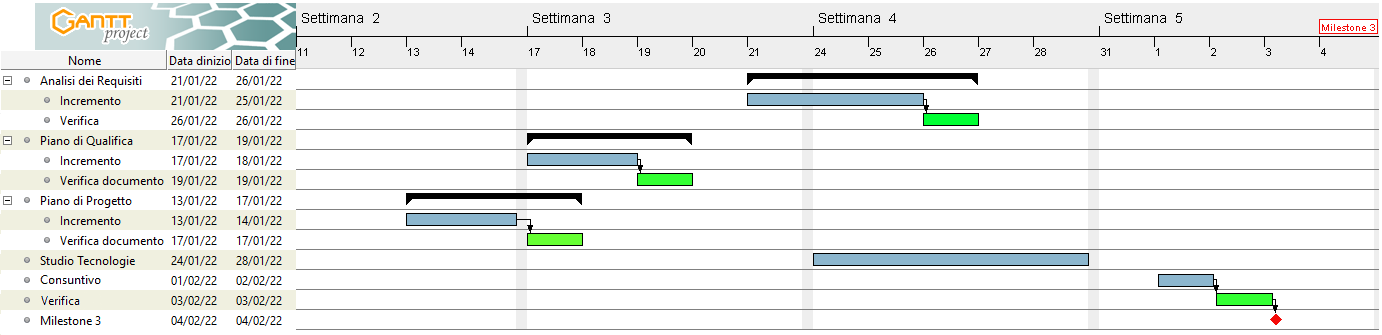
\includegraphics[width=1.0\textwidth]{Gantt3.png}
    \caption{Diagramma di Gantt della terza milestone}
\end{figure}


\subsection{Quarto periodo}
\textit{Periodo: 7/02/2022 - 24/02/2022}

In quest'ultimo periodo diventa di fondamentale importanza la progettazione e la realizzazione
 del PoC. Inoltre diviene necessario il completamento e la verifica finale dei documenti prima della revisione prevista
 per fine febbraio.


\begin{figure}[!ht]
    \includegraphics[width=1.0\textwidth]{Gantt4.png}
    \caption{Diagramma di Gantt della quarta milestone}
\end{figure}

\section{Verso la PB}

\textit{Periodo: 29/02/2022 - 04/04/2022}

Superata la prima revisione, l'obiettivo principale è realizzare una prima versione del prodotto finale che dimostri come ha già fatto il PoC, nella sua semplicità,
che requisiti e tecnologie scelte possono coesistere nello stesso prodotto.

Sarà, quindi, fondamentale la progettazione per arrivare ad avere un design$_G$ che sia quello definitivo e poi avere un avanzamento consistente di codifica e verifica.

Viste le difficoltà riscontrate nella pianificazione a lungo termine, preferiamo aspettare di superare la revisione precedente per poi poterci dedicare nel dettaglio
alla pianificazione dei periodi che caratterizzeranno l'intera milestone.

\subsection{Quinto periodo}
\textit{Periodo: 21/03/2022 - 28/03/2022}

In questo periodo, l'obiettivo è quello di sistemare gli errori emersi durante il colloquio dell'RTB, andando, in oltre, a esplorare i grafici non presenti nel PoC, per prepararsi a sviluppare il software.

\begin{figure}[!ht]
    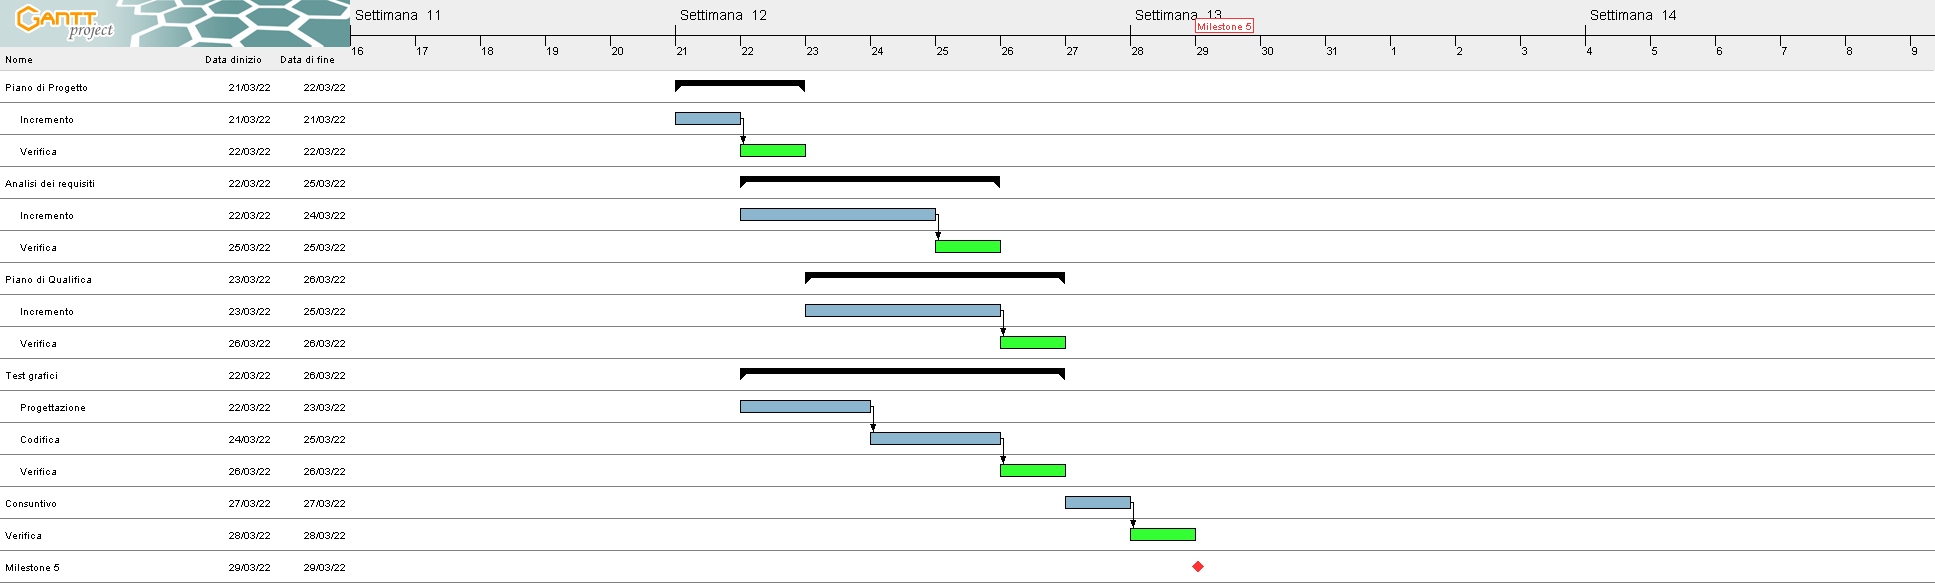
\includegraphics[width=1.0\textwidth]{Gantt5.png}
    \caption{Diagramma di Gantt della quinta milestone}
\end{figure}

\subsection{Sesto periodo}
\textit{Periodo: 29/03/2022 - 05/04/2022}

In questo periodo, il gruppo si è diviso in due sotto team. Un team si occuperà di progettare l'architettura del prodotto e l'altro aggiornerà i documenti in base alle necessità.

\begin{figure}[H]
    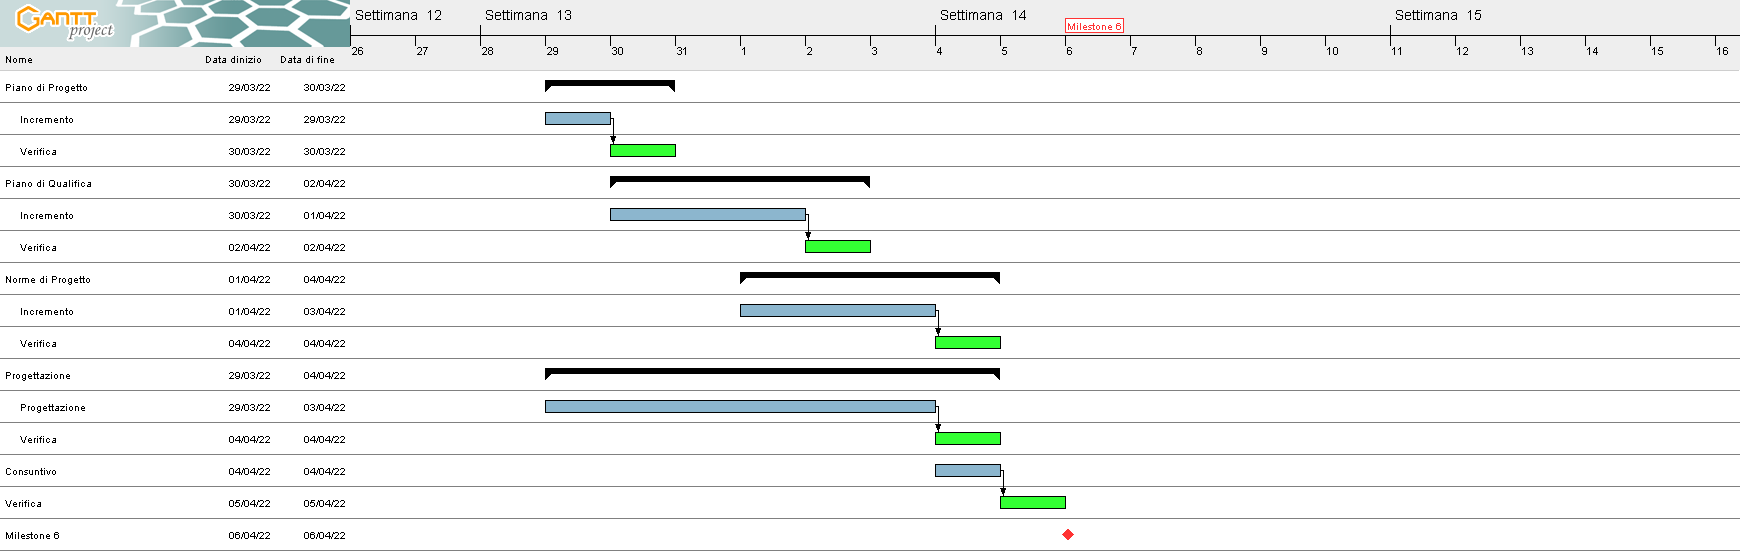
\includegraphics[width=1.0\textwidth]{Gantt6.png}
    \caption{Diagramma di Gantt della sesta milestone}
\end{figure}

\subsection{Settimo periodo}
\textit{Periodo: 06/04/2022 - 12/04/2022}

In questo periodo l'obiettivo principale è quello di portare a termine l'architettura finale del prodotto. Oltre a questo alcuni membri del gruppo inizieranno a codificare alcune parti del prodotto che sono indipendenti dall'architettura.

\subsection{Ottavo periodo}
\textit{Periodo: 13/04/2022 - 19/04/2022}

L'obiettivo del gruppo per questo periodo è quello di completare la parte iniziale di stesura del codice e di aggiornare i documenti.

\subsection{Nono periodo}
\textit{Periodo: 20/04/2022 - 26/04/2022}

Dopo aver codificato una buona parte di architettura, in questo periodo l'obiettivo è ritoccare l'architettura in base a quanto emerso nello sprint precedente per ultimare la \textit{Specifica Architetturale}. Successivamente si andrà a sistemare il codice e a integrarlo con le parti mancanti.

\section{Verso la CA}

\textit{Periodo: 05/04/2022 - 02/05/2022}

Superata la seconda revisione, l'obiettivo rimane quello di presentare al proponente il prodotto finale.

Sarà quindi necessario adattare il prodotto realizzato ai feedback$_G$ ricevuti nella revisione precedente e fare in modo che il prodotto superi tutti i test. Inoltre, bisognerà
verificare che il prodotto rispecchi le richieste del proponente poichè dovrà superare un vero e proprio collaudo.

Anche in questo caso, la pianificazione nel dettaglio sarà fatta in un secondo momento più opportuno e in condizioni migliori.

  \chapter{Preventivo}

\section{Verso la RTB}

\subsection{Primo periodo}

In questa fase i ruoli da ricoprire per portare a termine gli obiettivi
pianificati sono:
\begin{itemize}
    \item \textit{Responsabile};
    \item \textit{Amministratore};
    \item \textit{Verificatore}.
\end{itemize}

\subsubsection{Preventivo orario}

\begin{table}[H]
    \renewcommand\arraystretch{1.5}
    \centering
    \begin{tabular}{|l|c|c|c|c|c|c|c|}
    \hline
    \rowcolor[HTML]{036400}
    \textcolor{white}{\textbf{Membro}} & \multicolumn{1}{l|}{\textcolor{white}{\textbf{RE}}} & \multicolumn{1}{l|}{\textcolor{white}{\textbf{AM}}} & \multicolumn{1}{l|}{\textcolor{white}{\textbf{AN}}} & \multicolumn{1}{l|}{\textcolor{white}{\textbf{PT}}} & \multicolumn{1}{l|}{\textcolor{white}{\textbf{PR}}} & \multicolumn{1}{l|}{\textcolor{white}{\textbf{VE}}} & \multicolumn{1}{l|}{\textcolor{white}{\textbf{Totale ore persona}}} \\ \hline
    \rowcolor[HTML]{EFEFEF}\textit{Marco Mazzucato}  & 2 & 3  & - & - & - & 1 & 6  \\ \hline
    \rowcolor[HTML]{C0C0C0}\textit{Marco Mamprin}    & - & 3  & - & - & - & 1 & 4  \\ \hline
    \rowcolor[HTML]{EFEFEF}\textit{Marko Vukovic}    & 2 & 3  & - & - & - & 1 & 6  \\ \hline
    \rowcolor[HTML]{C0C0C0}\textit{Mattia Zanellato} & - & 3  & - & - & - & 1 & 4  \\ \hline
    \rowcolor[HTML]{EFEFEF}\textit{Emanuele Pase}    & - & 3  & - & - & - & 1 & 4  \\ \hline
    \rowcolor[HTML]{C0C0C0}\textit{Riccardo Contin}  & - & 3  & - & - & - & 1 & 4  \\ \hline
    \rowcolor[HTML]{EFEFEF}\textit{Lorenzo Onelia}   & - & 3  & - & - & - & 1 & 4  \\ \hline
    \textbf{Totale ore ruolo} & 4 & 21 & - & - & - & 7 & 32 \\ \hline
    \end{tabular}
    \caption{Distribuzione delle ore per la prima milestone}
\end{table}

\begin{figure}[H]
    \includegraphics[width=1.0\textwidth]{Istogramma1.jpg}
    \caption{Istogramma della distribuzione delle ore per la prima milestone}
\end{figure}

\begin{figure}[H]
    \includegraphics[width=1.0\textwidth]{Torta1.1.jpg}
    \caption{Grafico a torta della distribuzione delle ore per la prima milestone}
\end{figure}

\newpage
\subsubsection{Preventivo economico}

\begin{table}[H]
    \renewcommand\arraystretch{1.5}
    \centering
    \begin{tabular}{|l|c|c|}
    \hline
    \rowcolor[HTML]{036400}
    \textcolor{white}{\textbf{Ruolo}} & \multicolumn{1}{l|}{\textcolor{white}{\textbf{Ore}}} & \multicolumn{1}{l|}{\textcolor{white}{\textbf{Costo (€)}}} \\ \hline
    \rowcolor[HTML]{EFEFEF}\textit{Responsabile} & 4 & 120 \\ \hline
    \rowcolor[HTML]{C0C0C0}\textit{Amministratore} & 21 & 420 \\ \hline
    \rowcolor[HTML]{EFEFEF}\textit{Analista} & - & - \\ \hline
    \rowcolor[HTML]{C0C0C0}\textit{Progettista} & - & - \\ \hline
    \rowcolor[HTML]{EFEFEF}\textit{Programmatore} & - & - \\ \hline
    \rowcolor[HTML]{C0C0C0}\textit{Verificatore} & 7 & 105 \\ \hline
    \rowcolor[HTML]{EFEFEF}\textbf{Totale} & 32 & 645 \\ \hline
    \end{tabular}
    \caption{Prospetto dei costi per la prima milestone}
\end{table}

\begin{figure}[H]
    \includegraphics[width=1.0\textwidth]{Torta1.2.jpg}
    \caption{Grafico a torta della distribuzione dei costi per la prima milestone}
\end{figure}

\newpage
\subsection{Secondo periodo}

In questa fase i ruoli da ricoprire per portare a termine gli obiettivi
pianificati sono:
\begin{itemize}
    \item \textit{Responsabile};
    \item \textit{Amministratore};
    \item \textit{Analista};
    \item \textit{Verificatore}.
\end{itemize}

\subsubsection{Preventivo orario}

\begin{table}[H]
    \renewcommand\arraystretch{1.5}
    \centering
    \begin{tabular}{|l|c|c|c|c|c|c|c|}
    \hline
    \rowcolor[HTML]{036400}
    \textcolor{white}{\textbf{Membro}} & \multicolumn{1}{l|}{\textcolor{white}{\textbf{RE}}} & \multicolumn{1}{l|}{\textcolor{white}{\textbf{AM}}} & \multicolumn{1}{l|}{\textcolor{white}{\textbf{AN}}} & \multicolumn{1}{l|}{\textcolor{white}{\textbf{PT}}} & \multicolumn{1}{l|}{\textcolor{white}{\textbf{PR}}} & \multicolumn{1}{l|}{\textcolor{white}{\textbf{VE}}} & \multicolumn{1}{l|}{\textcolor{white}{\textbf{Totale ore persona}}} \\ \hline
    \rowcolor[HTML]{EFEFEF}\textit{Marco Mazzucato}  & - & 2   & 2  & - & - & 2  & 6   \\ \hline
    \rowcolor[HTML]{C0C0C0}\textit{Marco Mamprin}    & - & 2   & 1  & - & - & 2  & 5   \\ \hline
    \rowcolor[HTML]{EFEFEF}\textit{Marko Vukovic}    & - & 1.5 & 3  & - & - & 3  & 7.5 \\ \hline
    \rowcolor[HTML]{C0C0C0}\textit{Mattia Zanellato} & - & -   & 3  & - & - & 3  & 6   \\ \hline
    \rowcolor[HTML]{EFEFEF}\textit{Emanuele Pase}    & - & -   & 3  & - & - & 3  & 6   \\ \hline
    \rowcolor[HTML]{C0C0C0}\textit{Riccardo Contin}  & 4 & -   & 3  & - & - & 1  & 8   \\ \hline
    \rowcolor[HTML]{EFEFEF}\textit{Lorenzo Onelia}   & - & 2   & 2  & - & - & 3  & 7   \\ \hline
    \rowcolor[HTML]{C0C0C0}\textbf{Totale ore ruolo} & 4 & 7.5 & 17 & - & - & 17 & 45.5\\ \hline
    \end{tabular}
    \caption{Distribuzione delle ore per la seconda milestone}
\end{table}

\begin{figure}[H]
    \includegraphics[width=1.0\textwidth]{Istogramma2.jpg}
    \caption{Istogramma della distribuzione delle ore per la seconda milestone}
\end{figure}

\begin{figure}[H]
    \includegraphics[width=1.0\textwidth]{Torta2.1.jpg}
    \caption{Grafico a torta della distribuzione delle ore per la seconda milestone}
\end{figure}

\newpage
\subsubsection{Preventivo economico}

\begin{table}[H]
    \renewcommand\arraystretch{1.5}
    \centering
    \begin{tabular}{|l|c|c|}
    \hline
    \rowcolor[HTML]{036400}
    \textcolor{white}{\textbf{Ruolo}} & \multicolumn{1}{l|}{\textcolor{white}{\textbf{Ore}}} & \multicolumn{1}{l|}{\textcolor{white}{\textbf{Costo (€)}}} \\ \hline
    \rowcolor[HTML]{EFEFEF}\textit{Responsabile} & 4 & 120 \\ \hline
    \rowcolor[HTML]{C0C0C0}\textit{Amministratore} & 7.5 & 150 \\ \hline
    \rowcolor[HTML]{EFEFEF}\textit{Analista} & 17 & 425 \\ \hline
    \rowcolor[HTML]{C0C0C0}\textit{Progettista} & - & - \\ \hline
    \rowcolor[HTML]{EFEFEF}\textit{Programmatore} & - & - \\ \hline
    \rowcolor[HTML]{C0C0C0}\textit{Verificatore} & 17 & 255 \\ \hline
    \rowcolor[HTML]{EFEFEF}\textbf{Totale} & 45.5 & 950 \\ \hline
    \end{tabular}
    \caption{Prospetto dei costi per la seconda milestone}
\end{table}

\begin{figure}[H]
    \includegraphics[width=1.0\textwidth]{Torta2.2.jpg}
    \caption{Grafico a torta della distribuzione dei costi per la seconda milestone}
\end{figure}



\newpage
\subsection{Terzo periodo}

In questa fase i ruoli da ricoprire per portare a termine gli obiettivi
pianificati sono:
\begin{itemize}
    \item \textit{Responsabile};
    \item \textit{Amministratore};
    \item \textit{Analista};
    \item \textit{Progettista};
    \item \textit{Verificatore}.
\end{itemize}

\subsubsection{Preventivo orario}

\begin{table}[H]
    \renewcommand\arraystretch{1.5}
    \centering
    \begin{tabular}{|l|c|c|c|c|c|c|c|}
    \hline
    \rowcolor[HTML]{036400}
    \textcolor{white}{\textbf{Membro}} & \multicolumn{1}{l|}{\textcolor{white}{\textbf{RE}}} & \multicolumn{1}{l|}{\textcolor{white}{\textbf{AM}}} & \multicolumn{1}{l|}{\textcolor{white}{\textbf{AN}}} & \multicolumn{1}{l|}{\textcolor{white}{\textbf{PT}}} & \multicolumn{1}{l|}{\textcolor{white}{\textbf{PR}}} & \multicolumn{1}{l|}{\textcolor{white}{\textbf{VE}}} & \multicolumn{1}{l|}{\textcolor{white}{\textbf{Totale ore persona}}} \\ \hline
    \rowcolor[HTML]{EFEFEF}\textit{Marco Mazzucato}  & - & 1   & 1.5 & 2 & -  & 2    & 6.5  \\ \hline
    \rowcolor[HTML]{C0C0C0}\textit{Marco Mamprin}    & - & 1   & 2   & 2 & -  & 2    & 7    \\ \hline
    \rowcolor[HTML]{EFEFEF}\textit{Marko Vukovic}    & - & 1.5 & 2   & 2 & -  & 2    & 7.5  \\ \hline
    \rowcolor[HTML]{C0C0C0}\textit{Mattia Zanellato} & - & 1   & 2   & 2 & -  & 2    & 7    \\ \hline
    \rowcolor[HTML]{EFEFEF}\textit{Emanuele Pase}    & 4 & 1   & 0.5 & 2 & -  & 1    & 8.5  \\ \hline
    \rowcolor[HTML]{C0C0C0}\textit{Riccardo Contin}  & - & 1   & 1.5 & 2 & -  & 2.5  & 7    \\ \hline
    \rowcolor[HTML]{EFEFEF}\textit{Lorenzo Onelia}   & - & 1   & 1.5 & 2 & -  & 2    & 6.5  \\ \hline
    \rowcolor[HTML]{C0C0C0}\textbf{Totale ore ruolo} & 4 & 7.5 & 11  & 14& - & 13.5 & 50   \\ \hline
    \end{tabular}
    \caption{Distribuzione delle ore per la terza milestone}
\end{table}

\begin{figure}[H]
    \includegraphics[width=1.0\textwidth]{Istogramma3.jpg}
    \caption{Istogramma della distribuzione delle ore per la terza milestone}
\end{figure}

\begin{figure}[H]
    \includegraphics[width=1.0\textwidth]{Torta3.1.jpg}
    \caption{Grafico a torta della distribuzione delle ore per la terza milestone}
\end{figure}

\newpage
\subsubsection{Preventivo economico}

\begin{table}[H]
    \renewcommand\arraystretch{1.5}
    \centering
    \begin{tabular}{|l|c|c|}
    \hline
    \rowcolor[HTML]{036400}
    \textcolor{white}{\textbf{Ruolo}} & \multicolumn{1}{l|}{\textcolor{white}{\textbf{Ore}}} & \multicolumn{1}{l|}{\textcolor{white}{\textbf{Costo (€)}}} \\ \hline
    \rowcolor[HTML]{EFEFEF}\textit{Responsabile}   & 4    & 120   \\ \hline
    \rowcolor[HTML]{C0C0C0}\textit{Amministratore} & 7.5  & 150   \\ \hline
    \rowcolor[HTML]{EFEFEF}\textit{Analista}       & 11   & 275   \\ \hline
    \rowcolor[HTML]{C0C0C0}\textit{Progettista}    & 14   & 350   \\ \hline
    \rowcolor[HTML]{EFEFEF}\textit{Programmatore}  & -    & -     \\ \hline
    \rowcolor[HTML]{C0C0C0}\textit{Verificatore}   & 13.5 & 202.5 \\ \hline
    \rowcolor[HTML]{EFEFEF}\textbf{Totale}         & 50   & 1097,5\\ \hline
    \end{tabular}
    \caption{Prospetto dei costi per la terza milestone}
\end{table}

\begin{figure}[H]
    \includegraphics[width=1.0\textwidth]{Torta3.2.jpg}
    \caption{Grafico a torta della distribuzione dei costi per la terza milestone}
\end{figure}



\newpage
\subsection{Quarto periodo}

In questa fase i ruoli da ricoprire per portare a termine gli obiettivi pianificati sono:
\begin{itemize}
    \item \textit{Responsabile};
    \item \textit{Amministratore};
    \item \textit{Analista};
    \item \textit{Progettista};
    \item \textit{Programmatore};
    \item \textit{Verificatore}.
\end{itemize}

\subsubsection{Preventivo orario}

\begin{table}[H]
    \renewcommand\arraystretch{1.5}
    \centering
    \begin{tabular}{|l|c|c|c|c|c|c|c|}
    \hline
    \rowcolor[HTML]{036400}
    \textcolor{white}{\textbf{Membro}} & \multicolumn{1}{l|}{\textcolor{white}{\textbf{RE}}} & \multicolumn{1}{l|}{\textcolor{white}{\textbf{AM}}} & \multicolumn{1}{l|}{\textcolor{white}{\textbf{AN}}} & \multicolumn{1}{l|}{\textcolor{white}{\textbf{PT}}} & \multicolumn{1}{l|}{\textcolor{white}{\textbf{PR}}} & \multicolumn{1}{l|}{\textcolor{white}{\textbf{VE}}} & \multicolumn{1}{l|}{\textcolor{white}{\textbf{Totale ore persona}}} \\ \hline
    \rowcolor[HTML]{EFEFEF}\textit{Marco Mazzucato}  & - & -   & 2     & 4  & 4   & 2    & 12     \\ \hline
    \rowcolor[HTML]{C0C0C0}\textit{Marco Mamprin}    & - & 1   & 2     & 4  & 5   & 3    & 15     \\ \hline
    \rowcolor[HTML]{EFEFEF}\textit{Marko Vukovic}    & - & -   & 1     & 4  & 4   & 4    & 13     \\ \hline
    \rowcolor[HTML]{C0C0C0}\textit{Mattia Zanellato} & 4 & 4   & 1.5   & 4  & -   & 4    & 17.5   \\ \hline
    \rowcolor[HTML]{EFEFEF}\textit{Emanuele Pase}    & - & -   & -     & 3  & 4   & 3    & 10     \\ \hline
    \rowcolor[HTML]{C0C0C0}\textit{Riccardo Contin}  & - & 3   & 1     & 3  & -   & 3.5  & 10.5   \\ \hline
    \rowcolor[HTML]{EFEFEF}\textit{Lorenzo Onelia}   & - & 3   & 3     & 3  & -   & 3    & 12     \\ \hline
    \rowcolor[HTML]{C0C0C0}\textbf{Totale ore ruolo} & 4 & 11  & 10.5  & 25 & 17  & 22.5 & 90     \\ \hline
    \end{tabular}
    \caption{Distribuzione delle ore per la quarta milestone}
\end{table}

\begin{figure}[H]
    \includegraphics[width=1.0\textwidth]{Istogramma4.jpg}
    \caption{Istogramma della distribuzione delle ore per la quarta milestone}
\end{figure}

\begin{figure}[H]
    \includegraphics[width=1.0\textwidth]{Torta4.1.jpg}
    \caption{Grafico a torta della distribuzione delle ore per la quarta milestone}
\end{figure}

\newpage
\subsubsection{Preventivo economico}

\begin{table}[H]
    \renewcommand\arraystretch{1.5}
    \centering
    \begin{tabular}{|l|c|c|}
    \hline
    \rowcolor[HTML]{036400}
    \textcolor{white}{\textbf{Ruolo}} & \multicolumn{1}{l|}{\textcolor{white}{\textbf{Ore}}} & \multicolumn{1}{l|}{\textcolor{white}{\textbf{Costo (€)}}} \\ \hline
    \rowcolor[HTML]{EFEFEF}\textit{Responsabile}   & 4    & 120     \\ \hline
    \rowcolor[HTML]{C0C0C0}\textit{Amministratore} & 11   & 220     \\ \hline
    \rowcolor[HTML]{EFEFEF}\textit{Analista}       & 10.5 & 262.5   \\ \hline
    \rowcolor[HTML]{C0C0C0}\textit{Progettista}    & 25   & 625     \\ \hline
    \rowcolor[HTML]{EFEFEF}\textit{Programmatore}  & 17   & 255     \\ \hline
    \rowcolor[HTML]{C0C0C0}\textit{Verificatore}   & 22.5 & 337.5   \\ \hline
    \rowcolor[HTML]{EFEFEF}\textbf{Totale}         & 90   & 1820    \\ \hline
    \end{tabular}
    \caption{Prospetto dei costi per la quarta milestone}
\end{table}

\begin{figure}[H]
    \includegraphics[width=1.0\textwidth]{Torta4.2.jpg}
    \caption{Grafico a torta della distribuzione dei costi per la quarta milestone}
\end{figure}

\newpage
\section{Verso la PB}

\subsection{Quinto periodo}

In questa fase i ruoli da ricoprire per portare a termine gli obiettivi pianificati sono:
\begin{itemize}
    \item \textit{Responsabile};
    \item \textit{Amministratore};
    \item \textit{Analista};
    \item \textit{Progettista};
    \item \textit{Programmatore};
    \item \textit{Verificatore}.
\end{itemize}

\subsubsection{Preventivo orario}

\begin{table}[H]
    \renewcommand\arraystretch{1.5}
    \centering
    \begin{tabular}{|l|c|c|c|c|c|c|c|}
    \hline
    \rowcolor[HTML]{036400}
    \textcolor{white}{\textbf{Membro}} & \multicolumn{1}{l|}{\textcolor{white}{\textbf{RE}}} & \multicolumn{1}{l|}{\textcolor{white}{\textbf{AM}}} & \multicolumn{1}{l|}{\textcolor{white}{\textbf{AN}}} & \multicolumn{1}{l|}{\textcolor{white}{\textbf{PT}}} & \multicolumn{1}{l|}{\textcolor{white}{\textbf{PR}}} & \multicolumn{1}{l|}{\textcolor{white}{\textbf{VE}}} & \multicolumn{1}{l|}{\textcolor{white}{\textbf{Totale ore persona}}} \\ \hline
    \rowcolor[HTML]{EFEFEF}\textit{Marco Mazzucato}  & - & 1   & -     & 2    & -    & 1    & 4     \\ \hline
    \rowcolor[HTML]{C0C0C0}\textit{Marco Mamprin}    & 2 & 1   & 1     & -    & 3    & 2    & 9     \\ \hline
    \rowcolor[HTML]{EFEFEF}\textit{Marko Vukovic}    & - & 2   & -     & -    & -    & 3    & 5     \\ \hline
    \rowcolor[HTML]{C0C0C0}\textit{Mattia Zanellato} & - & -   & -     & 3.5  & 4.5  & 1    & 9     \\ \hline
    \rowcolor[HTML]{EFEFEF}\textit{Emanuele Pase}    & - & -   & -     & 2    & -    & 2    & 4     \\ \hline
    \rowcolor[HTML]{C0C0C0}\textit{Riccardo Contin}  & - & -   & -     & 2    & 2    & 2    & 6     \\ \hline
    \rowcolor[HTML]{EFEFEF}\textit{Lorenzo Onelia}   & - & 0.5 & -     & 4    & 3    & 3.5  & 11    \\ \hline
    \rowcolor[HTML]{C0C0C0}\textbf{Totale ore ruolo} & 2 & 4.5 & 1     & 13.5 & 12.5 & 14.5 & 48    \\ \hline
    \end{tabular}
    \caption{Distribuzione delle ore per la quinta milestone}
\end{table}

\begin{figure}[H]
    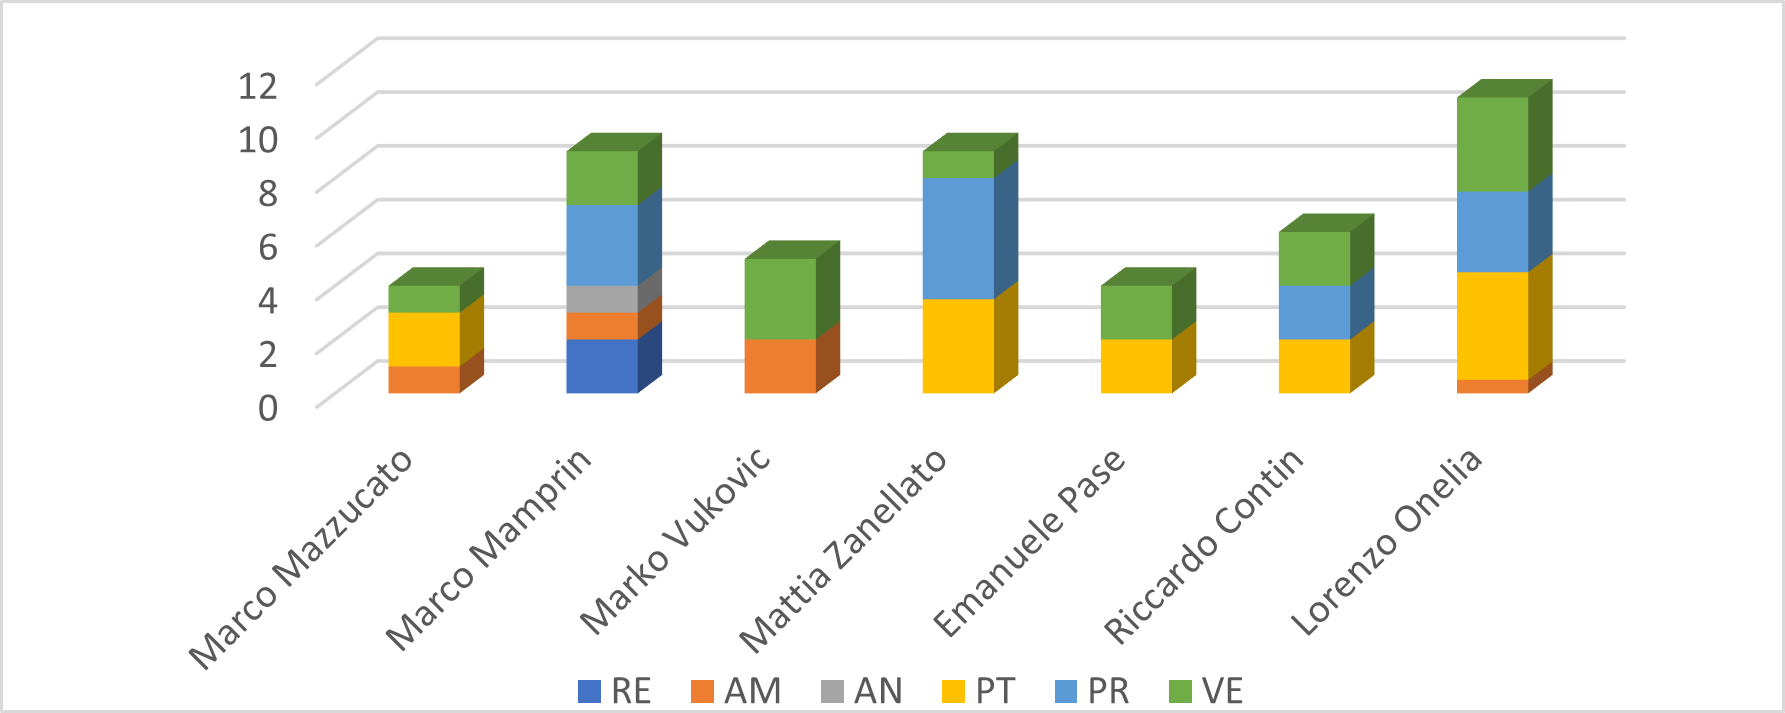
\includegraphics[width=1.0\textwidth]{Istogramma5.jpg}
    \caption{Istogramma della distribuzione delle ore per la quinta milestone}
\end{figure}

\begin{figure}[H]
    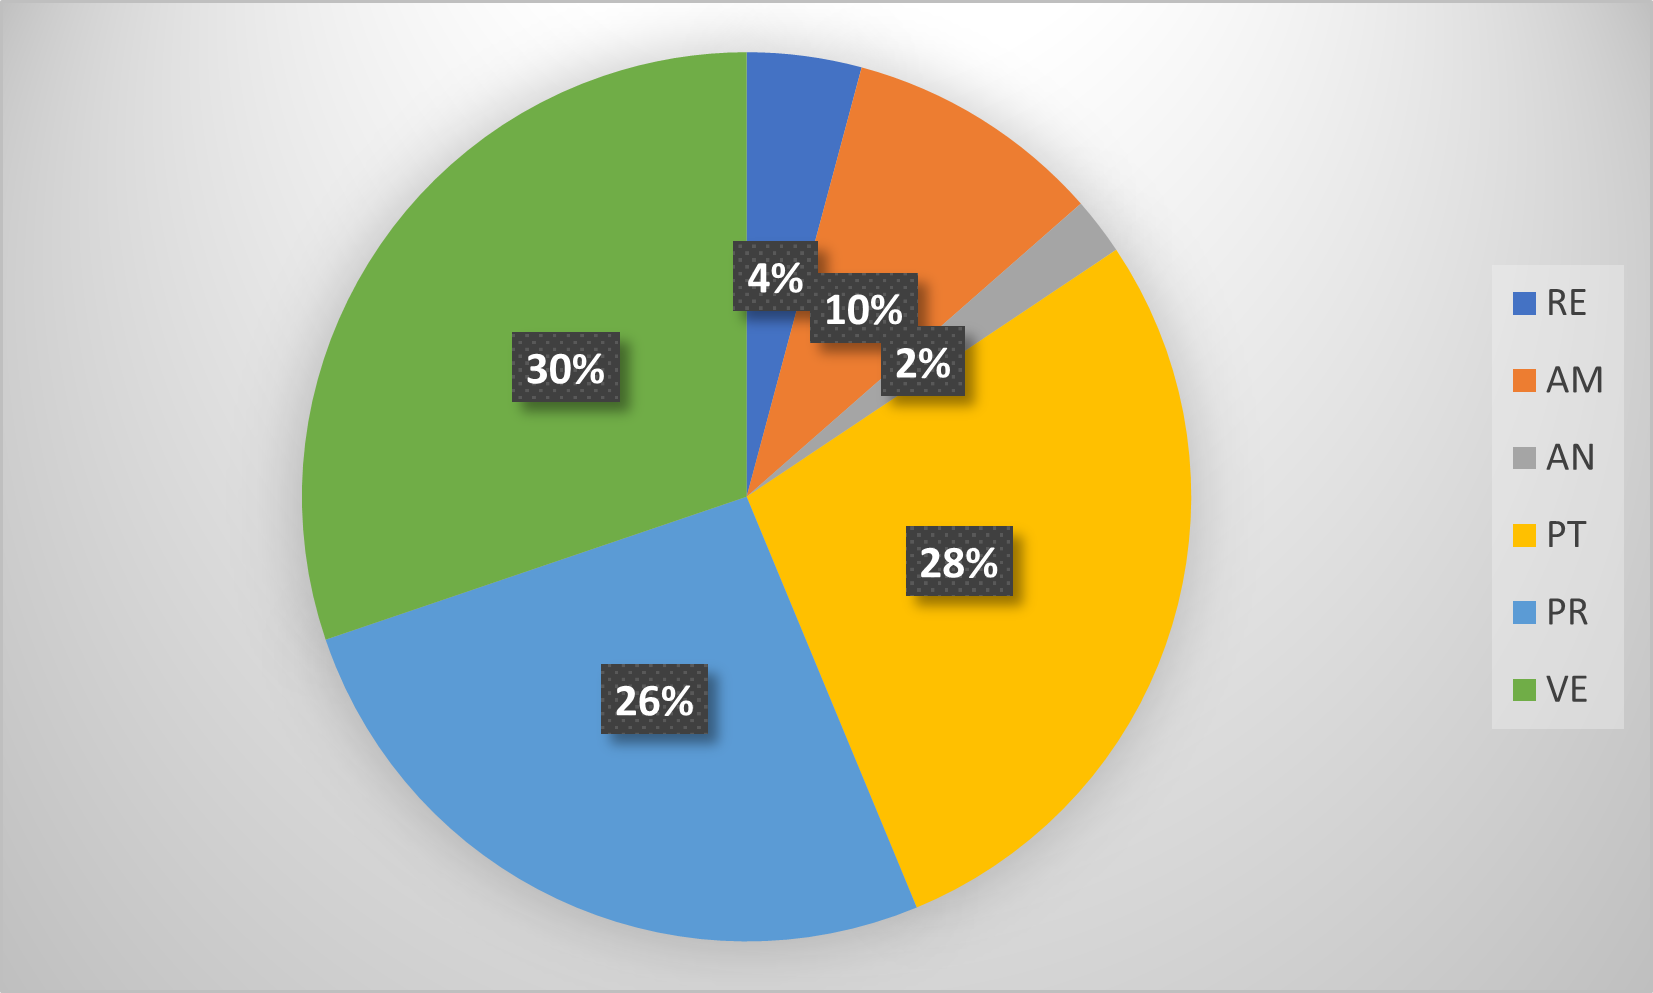
\includegraphics[width=1.0\textwidth]{Torta5.1.jpg}
    \caption{Grafico a torta della distribuzione delle ore per la quinta milestone}
\end{figure}

\newpage
\subsubsection{Preventivo economico}

\begin{table}[H]
    \renewcommand\arraystretch{1.5}
    \centering
    \begin{tabular}{|l|c|c|}
    \hline
    \rowcolor[HTML]{036400}
    \textcolor{white}{\textbf{Ruolo}} & \multicolumn{1}{l|}{\textcolor{white}{\textbf{Ore}}} & \multicolumn{1}{l|}{\textcolor{white}{\textbf{Costo (€)}}} \\ \hline
    \rowcolor[HTML]{EFEFEF}\textit{Responsabile}   & 2    & 60     \\ \hline
    \rowcolor[HTML]{C0C0C0}\textit{Amministratore} & 4.5  & 90     \\ \hline
    \rowcolor[HTML]{EFEFEF}\textit{Analista}       & 1    & 25     \\ \hline
    \rowcolor[HTML]{C0C0C0}\textit{Progettista}    & 13.5 & 337.5  \\ \hline
    \rowcolor[HTML]{EFEFEF}\textit{Programmatore}  & 12.5 & 187.5  \\ \hline
    \rowcolor[HTML]{C0C0C0}\textit{Verificatore}   & 14.5 & 217.5  \\ \hline
    \rowcolor[HTML]{EFEFEF}\textbf{Totale}         & 48   & 917.5  \\ \hline
    \end{tabular}
    \caption{Prospetto dei costi per la quinta milestone}
\end{table}

\begin{figure}[H]
    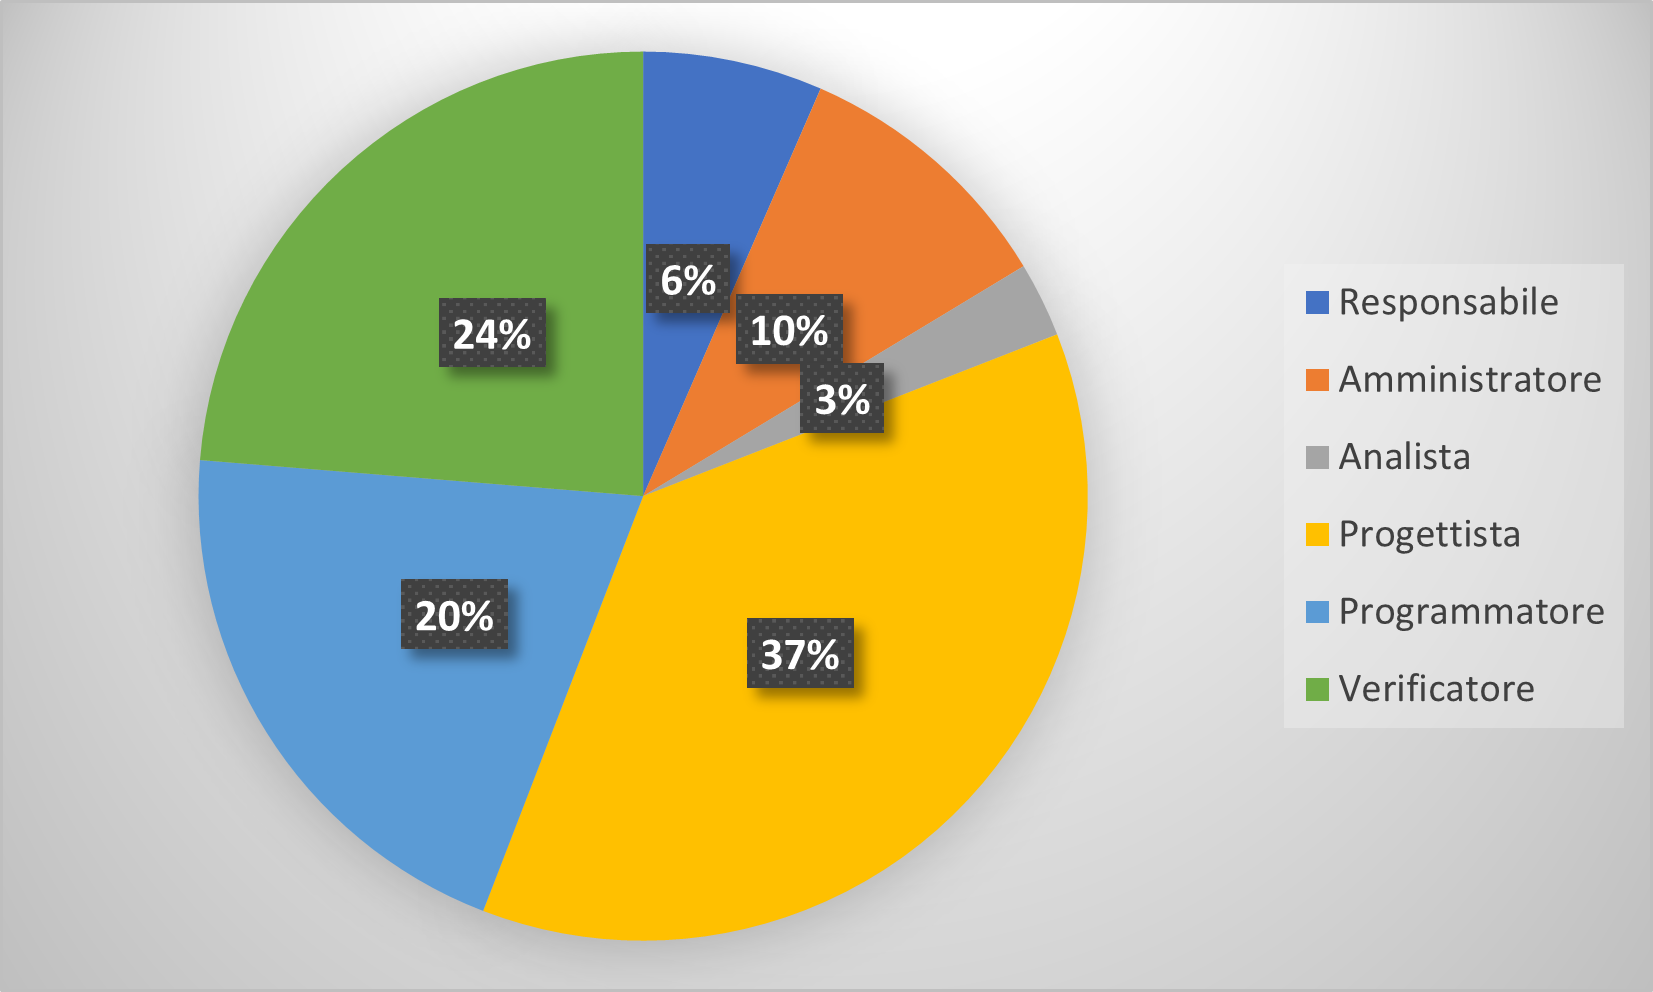
\includegraphics[width=1.0\textwidth]{Torta5.2.jpg}
    \caption{Grafico a torta della distribuzione dei costi per la quinta milestone}
\end{figure}

\subsection{Sesto periodo}

In questa fase i ruoli da ricoprire per portare a termine gli obiettivi pianificati sono:
\begin{itemize}
    \item \textit{Responsabile};
    \item \textit{Amministratore};
    \item \textit{Progettista};
    \item \textit{Programmatore};
    \item \textit{Verificatore}.
\end{itemize}

\subsubsection{Obiettivi}
Gli obiettivi di questo periodo sono:
\begin{itemize}
    \item Progettare l'architettura del prodotto;
    \item Aggiornare il documento \textit{Piano di Progetto};
    \item Aggiornare il documento \textit{Norme di Progetto};
    \item Aggiornare il documento \textit{Piano di Qualifica};
    \item Incontrare il proponente e risolvere i dubbi riscontrati nel meeting interno del 29/03/2022.
\end{itemize}

\subsubsection{Preventivo orario}

\begin{table}[H]
    \renewcommand\arraystretch{1.5}
    \centering
    \begin{tabular}{|l|c|c|c|c|c|c|c|}
    \hline
    \rowcolor[HTML]{036400}
    \textcolor{white}{\textbf{Membro}} & \multicolumn{1}{l|}{\textcolor{white}{\textbf{RE}}} & \multicolumn{1}{l|}{\textcolor{white}{\textbf{AM}}} & \multicolumn{1}{l|}{\textcolor{white}{\textbf{AN}}} & \multicolumn{1}{l|}{\textcolor{white}{\textbf{PT}}} & \multicolumn{1}{l|}{\textcolor{white}{\textbf{PR}}} & \multicolumn{1}{l|}{\textcolor{white}{\textbf{VE}}} & \multicolumn{1}{l|}{\textcolor{white}{\textbf{Totale ore persona}}} \\ \hline
    \rowcolor[HTML]{EFEFEF}\textit{Marco Mazzucato}  & - & 1   & -  & 10    & -   & 2   & 13     \\ \hline
    \rowcolor[HTML]{C0C0C0}\textit{Marco Mamprin}    & - & 1   & -  & 3     & 2   & 3   & 9     \\ \hline
    \rowcolor[HTML]{EFEFEF}\textit{Marko Vukovic}    & - & -   & -  & 12    & -   & 4   & 16     \\ \hline
    \rowcolor[HTML]{C0C0C0}\textit{Mattia Zanellato} & - & 1   & -  & 3     & 2   & 2   & 8     \\ \hline
    \rowcolor[HTML]{EFEFEF}\textit{Emanuele Pase}    & - & 2   & -  & 12    & -   & 1   & 15     \\ \hline
    \rowcolor[HTML]{C0C0C0}\textit{Riccardo Contin}  & - & -   & -  & 12    & -   & 2   & 14     \\ \hline
    \rowcolor[HTML]{EFEFEF}\textit{Lorenzo Onelia}   & 4 & -   & -  & 2     & 2   & 2   & 10    \\ \hline
    \rowcolor[HTML]{C0C0C0}\textbf{Totale ore ruolo} & 4 & 5   & 0  & 54    & 6   & 16  & 85    \\ \hline
    \end{tabular}
    \caption{Distribuzione delle ore per la sesta milestone}
\end{table}

\begin{figure}[H]
    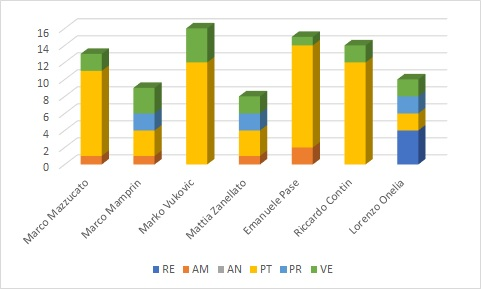
\includegraphics[width=1.0\textwidth]{Istogramma6.jpg}
    \caption{Istogramma della distribuzione delle ore per la sesta milestone}
\end{figure}

\begin{figure}[H]
    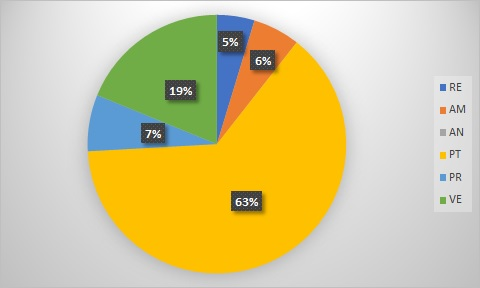
\includegraphics[width=1.0\textwidth]{Torta6.1.jpg}
    \caption{Grafico a torta della distribuzione delle ore per la sesta milestone}
\end{figure}

\newpage
\subsubsection{Preventivo economico}

\begin{table}[H]
    \renewcommand\arraystretch{1.5}
    \centering
    \begin{tabular}{|l|c|c|}
    \hline
    \rowcolor[HTML]{036400}
    \textcolor{white}{\textbf{Ruolo}} & \multicolumn{1}{l|}{\textcolor{white}{\textbf{Ore}}} & \multicolumn{1}{l|}{\textcolor{white}{\textbf{Costo (€)}}} \\ \hline
    \rowcolor[HTML]{EFEFEF}\textit{Responsabile}   & 4    & 120     \\ \hline
    \rowcolor[HTML]{C0C0C0}\textit{Amministratore} & 5  & 100     \\ \hline
    \rowcolor[HTML]{EFEFEF}\textit{Analista}       & 0    & 0     \\ \hline
    \rowcolor[HTML]{C0C0C0}\textit{Progettista}    & 54 & 1350  \\ \hline
    \rowcolor[HTML]{EFEFEF}\textit{Programmatore}  & 6 & 90  \\ \hline
    \rowcolor[HTML]{C0C0C0}\textit{Verificatore}   & 16 & 240  \\ \hline
    \rowcolor[HTML]{EFEFEF}\textbf{Totale}         & 85   & 1900  \\ \hline
    \end{tabular}
    \caption{Prospetto dei costi per la sesta milestone}
\end{table}

\begin{figure}[H]
    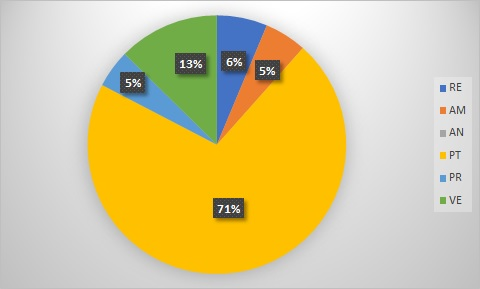
\includegraphics[width=1.0\textwidth]{Torta6.2.jpg}
    \caption{Grafico a torta della distribuzione dei costi per la sesta milestone}
\end{figure}

\subsection{Settimo periodo}

In questa fase i ruoli da ricoprire per portare a termine gli obiettivi pianificati sono:
\begin{itemize}
    \item \textit{Responsabile};
    \item \textit{Analista};
    \item \textit{Progettista};
    \item \textit{Programmatore};
    \item \textit{Verificatore}.
\end{itemize}

\subsubsection{Obiettivi}
Gli obiettivi di questo periodo sono:
\begin{itemize}
    \item Finire la progettazione dell'architettura del prodotto;
    \item Aggiornare il documento \textit{Norme di Progetto};
    \item Codificare le varie funzioni che disegnano i grafici;
    \item Trovare un adeguato algoritmo di campionamento;
    \item Incontrare il proponente per discutere dell'architettura e chiedere dei consigli sulla visualizzazione dei grafici.
\end{itemize}

\subsubsection{Preventivo orario}

\begin{table}[H]
    \renewcommand\arraystretch{1.5}
    \centering
    \begin{tabular}{|l|c|c|c|c|c|c|c|}
    \hline
    \rowcolor[HTML]{036400}
    \textcolor{white}{\textbf{Membro}} & \multicolumn{1}{l|}{\textcolor{white}{\textbf{RE}}} & \multicolumn{1}{l|}{\textcolor{white}{\textbf{AM}}} & \multicolumn{1}{l|}{\textcolor{white}{\textbf{AN}}} & \multicolumn{1}{l|}{\textcolor{white}{\textbf{PT}}} & \multicolumn{1}{l|}{\textcolor{white}{\textbf{PR}}} & \multicolumn{1}{l|}{\textcolor{white}{\textbf{VE}}} & \multicolumn{1}{l|}{\textcolor{white}{\textbf{Totale ore persona}}} \\ \hline
    \rowcolor[HTML]{EFEFEF}\textit{Marco Mazzucato}  & 6 & -   & -  & 4.5  & 4   & 3    & 17.5     \\ \hline
    \rowcolor[HTML]{C0C0C0}\textit{Marco Mamprin}    & - & -   & -  & 4    & 3   & 2    & 9     \\ \hline
    \rowcolor[HTML]{EFEFEF}\textit{Marko Vukovic}    & - & -   & -  & 4    & 6   & 2    & 12     \\ \hline
    \rowcolor[HTML]{C0C0C0}\textit{Mattia Zanellato} & - & -   & -  & 3    & 5   & 2    & 10     \\ \hline
    \rowcolor[HTML]{EFEFEF}\textit{Emanuele Pase}    & - & -   & -  & 5    & 4   & 2.5  & 11.5     \\ \hline
    \rowcolor[HTML]{C0C0C0}\textit{Riccardo Contin}  & - & -   & 1  & 3    & 5   & 2    & 11     \\ \hline
    \rowcolor[HTML]{EFEFEF}\textit{Lorenzo Onelia}   & - & -   & -  & 6    & 3   & 2    & 11    \\ \hline
    \rowcolor[HTML]{C0C0C0}\textbf{Totale ore ruolo} & 6 & 0   & 1  & 29.5 & 30  & 15.5 & 82    \\ \hline
    \end{tabular}
    \caption{Distribuzione delle ore per la settima milestone}
\end{table}

\begin{figure}[H]
    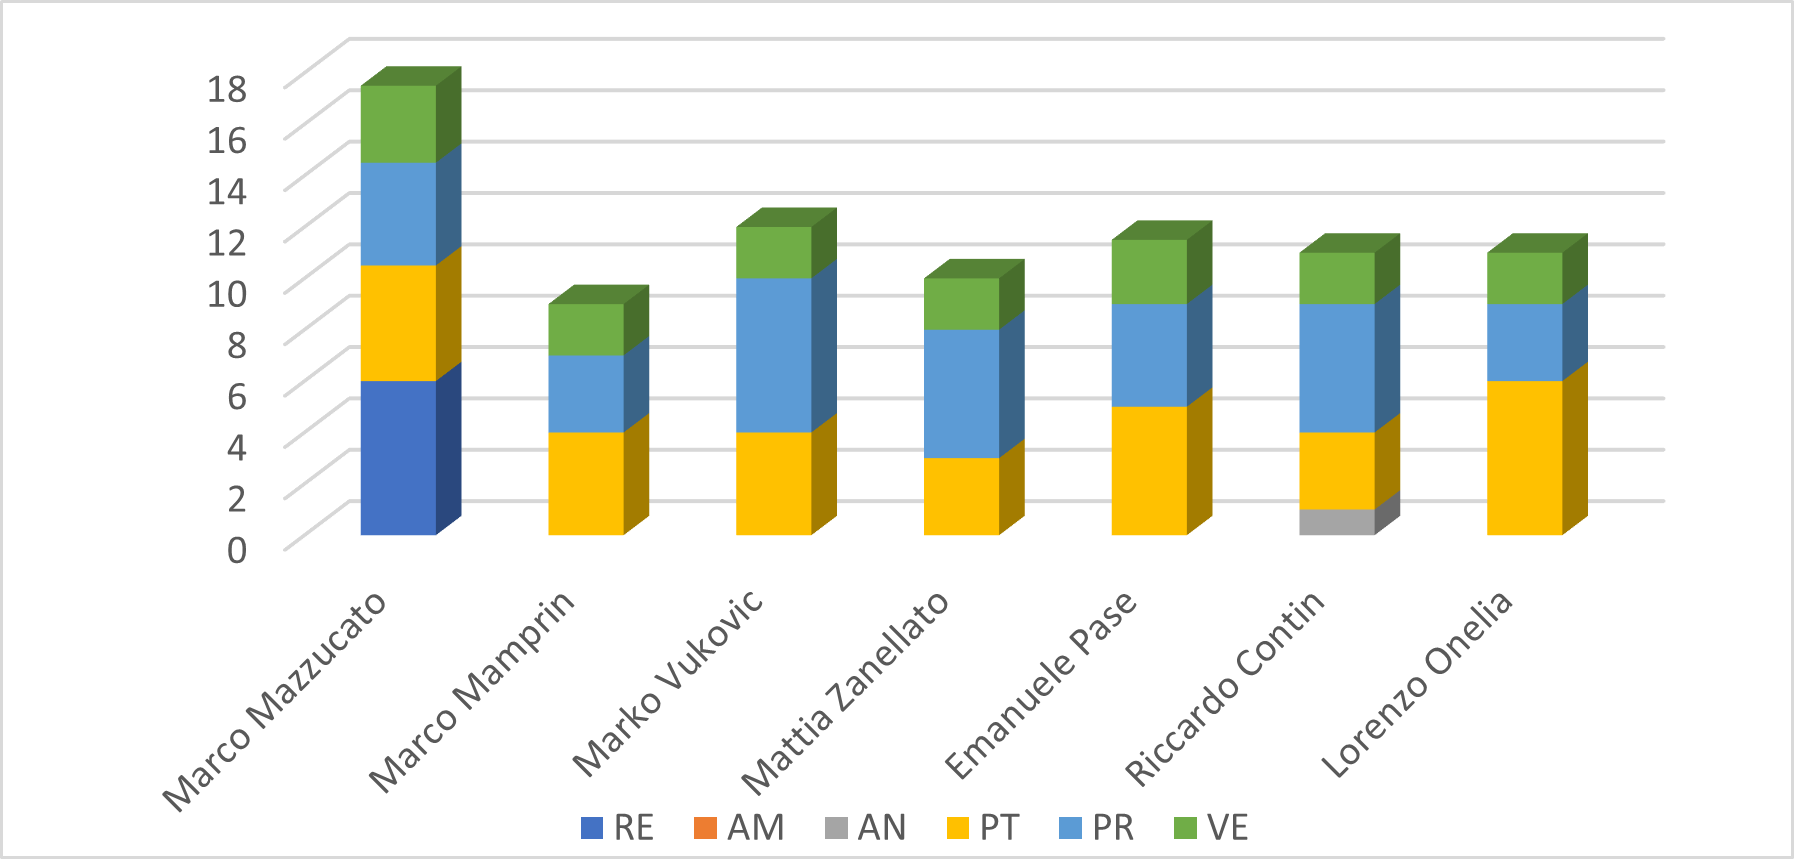
\includegraphics[width=1.0\textwidth]{Istogramma7.png}
    \caption{Istogramma della distribuzione delle ore per la settima milestone}
\end{figure}

\begin{figure}[H]
    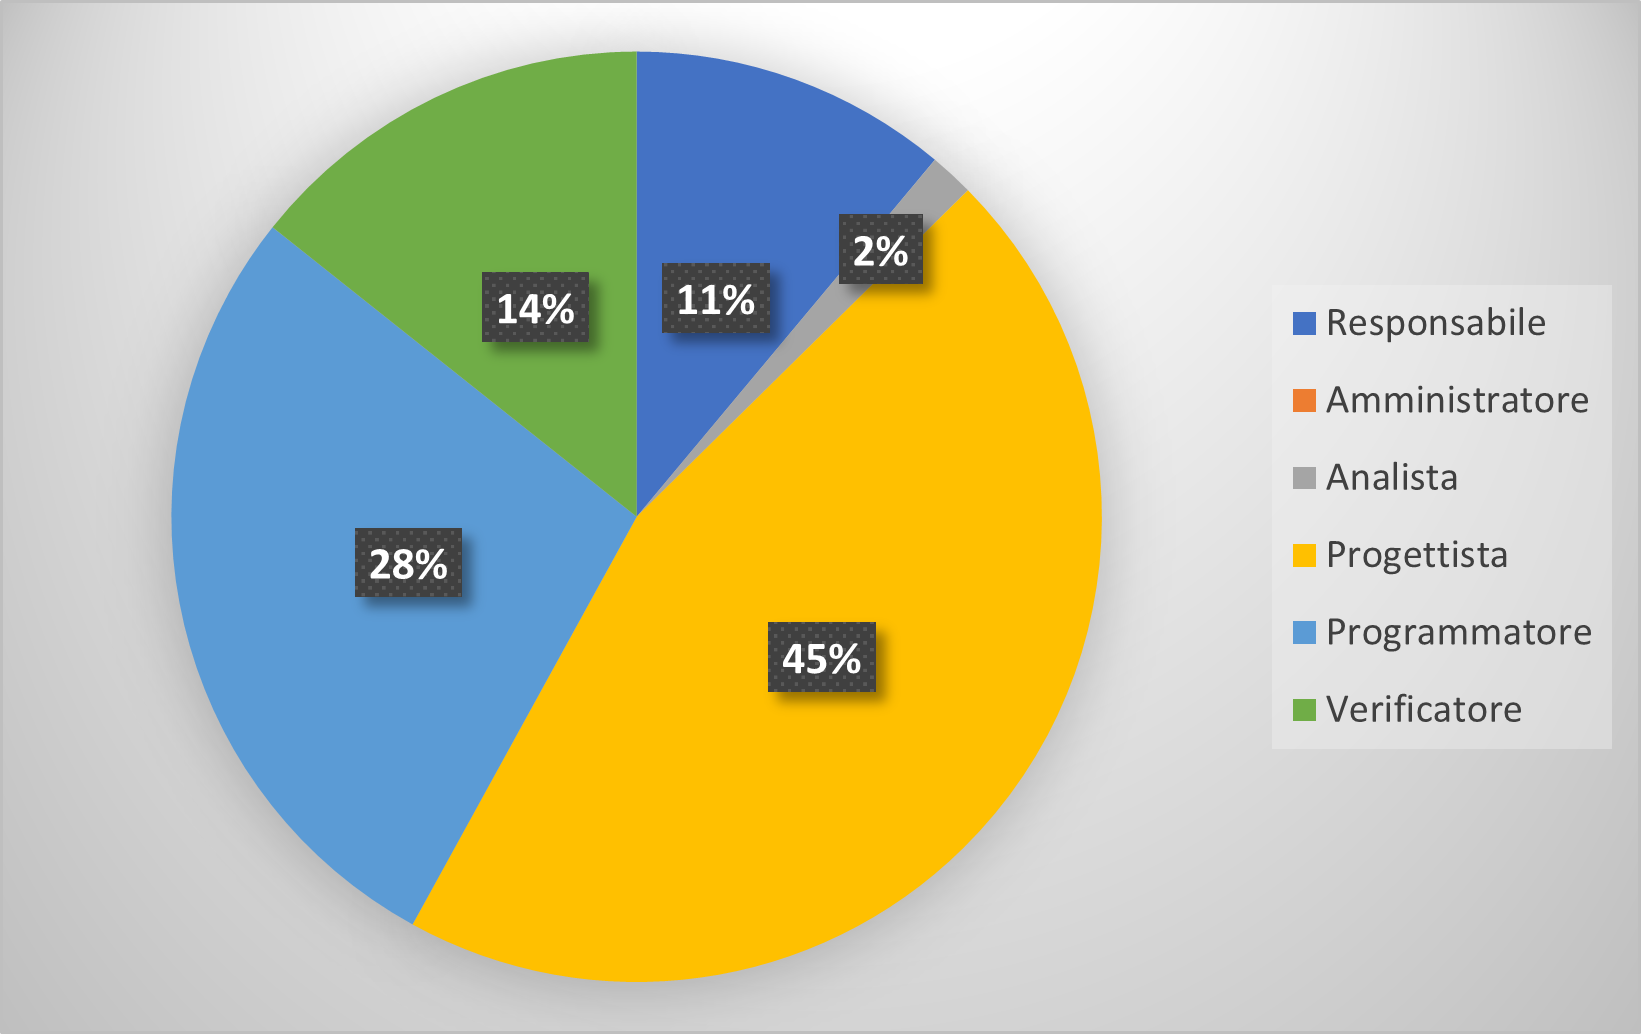
\includegraphics[width=1.0\textwidth]{Torta7.1.png}
    \caption{Grafico a torta della distribuzione delle ore per la settima milestone}
\end{figure}

\newpage
\subsubsection{Preventivo economico}

\begin{table}[H]
    \renewcommand\arraystretch{1.5}
    \centering
    \begin{tabular}{|l|c|c|}
    \hline
    \rowcolor[HTML]{036400}
    \textcolor{white}{\textbf{Ruolo}} & \multicolumn{1}{l|}{\textcolor{white}{\textbf{Ore}}} & \multicolumn{1}{l|}{\textcolor{white}{\textbf{Costo (€)}}} \\ \hline
    \rowcolor[HTML]{EFEFEF}\textit{Responsabile}   & 6    & 180     \\ \hline
    \rowcolor[HTML]{C0C0C0}\textit{Amministratore} & 0  & 0     \\ \hline
    \rowcolor[HTML]{EFEFEF}\textit{Analista}       & 1    & 25     \\ \hline
    \rowcolor[HTML]{C0C0C0}\textit{Progettista}    & 29.5 & 737.5  \\ \hline
    \rowcolor[HTML]{EFEFEF}\textit{Programmatore}  & 30 & 450  \\ \hline
    \rowcolor[HTML]{C0C0C0}\textit{Verificatore}   & 15.5 & 232.5  \\ \hline
    \rowcolor[HTML]{EFEFEF}\textbf{Totale}         & 82   & 1625  \\ \hline
    \end{tabular}
    \caption{Prospetto dei costi per la settima milestone}
\end{table}

\begin{figure}[H]
    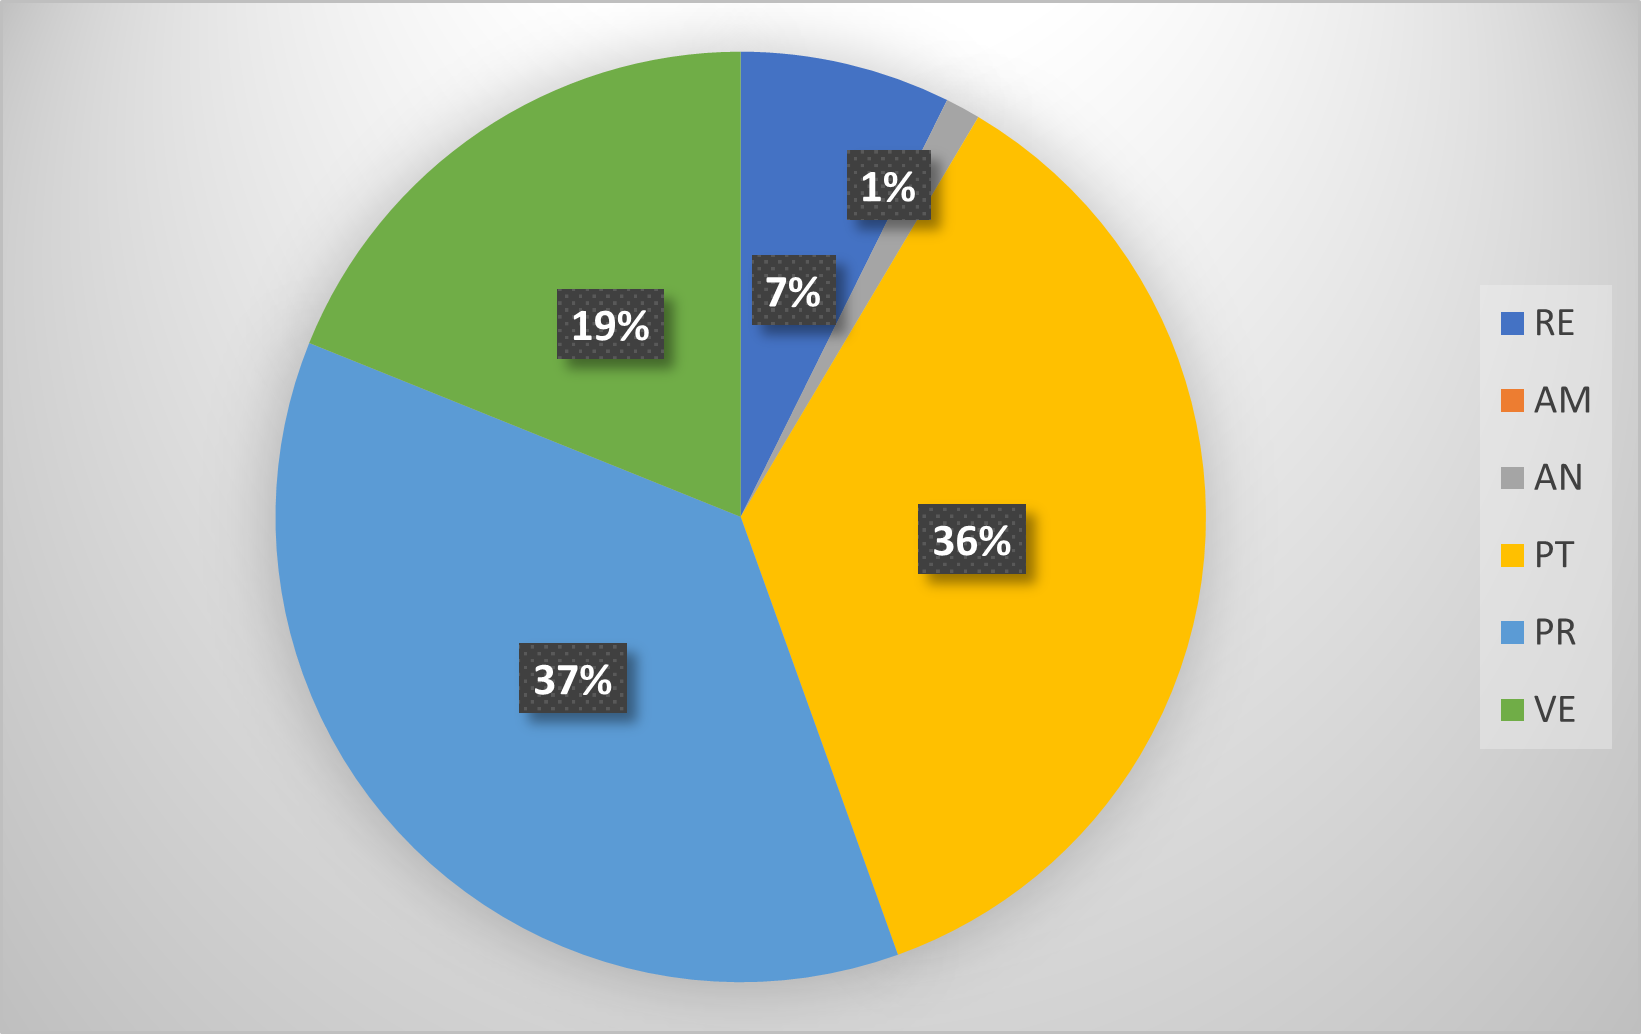
\includegraphics[width=1.0\textwidth]{Torta7.2.png}
    \caption{Grafico a torta della distribuzione dei costi per la settima milestone}
\end{figure}



\subsection{Ottavo periodo}

In questa fase i ruoli da ricoprire per portare a termine gli obiettivi pianificati sono:
\begin{itemize}
    \item \textit{Responsabile};
    \item \textit{Amministratore};
    \item \textit{Progettista};
    \item \textit{Programmatore};
    \item \textit{Verificatore}.
\end{itemize}

\subsubsection{Obiettivi}
Gli obiettivi di questo periodo sono:
\begin{itemize}
    \item Finire la progettazione modellando il diagramma di sequenza;
    \item Finire la codifica della classe "IndexedDBStorage";
    \item Codificare "Customization" e "Visualization" del diagramma delle classi;
    \item Codificare "Home Controller" e "VisualizationController" del diagramma delle classi;
    \item Codificare la parte rimanente della View;
    \item Identificare nuovi algoritmi di campionamento;
    \item Aggiornare il Cruscotto.
\end{itemize}

\subsubsection{Preventivo orario}

\begin{table}[H]
    \renewcommand\arraystretch{1.5}
    \centering
    \begin{tabular}{|l|c|c|c|c|c|c|c|}
    \hline
    \rowcolor[HTML]{036400}
    \textcolor{white}{\textbf{Membro}} & \multicolumn{1}{l|}{\textcolor{white}{\textbf{RE}}} & \multicolumn{1}{l|}{\textcolor{white}{\textbf{AM}}} & \multicolumn{1}{l|}{\textcolor{white}{\textbf{AN}}} & \multicolumn{1}{l|}{\textcolor{white}{\textbf{PT}}} & \multicolumn{1}{l|}{\textcolor{white}{\textbf{PR}}} & \multicolumn{1}{l|}{\textcolor{white}{\textbf{VE}}} & \multicolumn{1}{l|}{\textcolor{white}{\textbf{Totale ore persona}}} \\ \hline
    \rowcolor[HTML]{EFEFEF}\textit{Marco Mazzucato}  & - & 1.5 & -  & -    & 8   & 3    & 12.5     \\ \hline
    \rowcolor[HTML]{C0C0C0}\textit{Marco Mamprin}    & - & -   & -  & 4    & 5   & 3    & 12     \\ \hline
    \rowcolor[HTML]{EFEFEF}\textit{Marko Vukovic}    & - & -   & -  & -    & 10  & -    & 10     \\ \hline
    \rowcolor[HTML]{C0C0C0}\textit{Mattia Zanellato} & - & -   & -  & 3    & 6   & 2    & 11     \\ \hline
    \rowcolor[HTML]{EFEFEF}\textit{Emanuele Pase}    & 5 & -   & -  & -    & 6   & 5    & 16     \\ \hline
    \rowcolor[HTML]{C0C0C0}\textit{Riccardo Contin}  & - & -   & -  & 2    & 6   & 2    & 10     \\ \hline
    \rowcolor[HTML]{EFEFEF}\textit{Lorenzo Onelia}   & - & -   & -  & 2    & 7   & 2    & 11    \\ \hline
    \rowcolor[HTML]{C0C0C0}\textbf{Totale ore ruolo} & 5 & 1.5 & 0  & 11   & 48  & 17   & 82.5    \\ \hline
    \end{tabular}
    \caption{Distribuzione delle ore per l'ottava milestone}
\end{table}

\begin{figure}[H]
    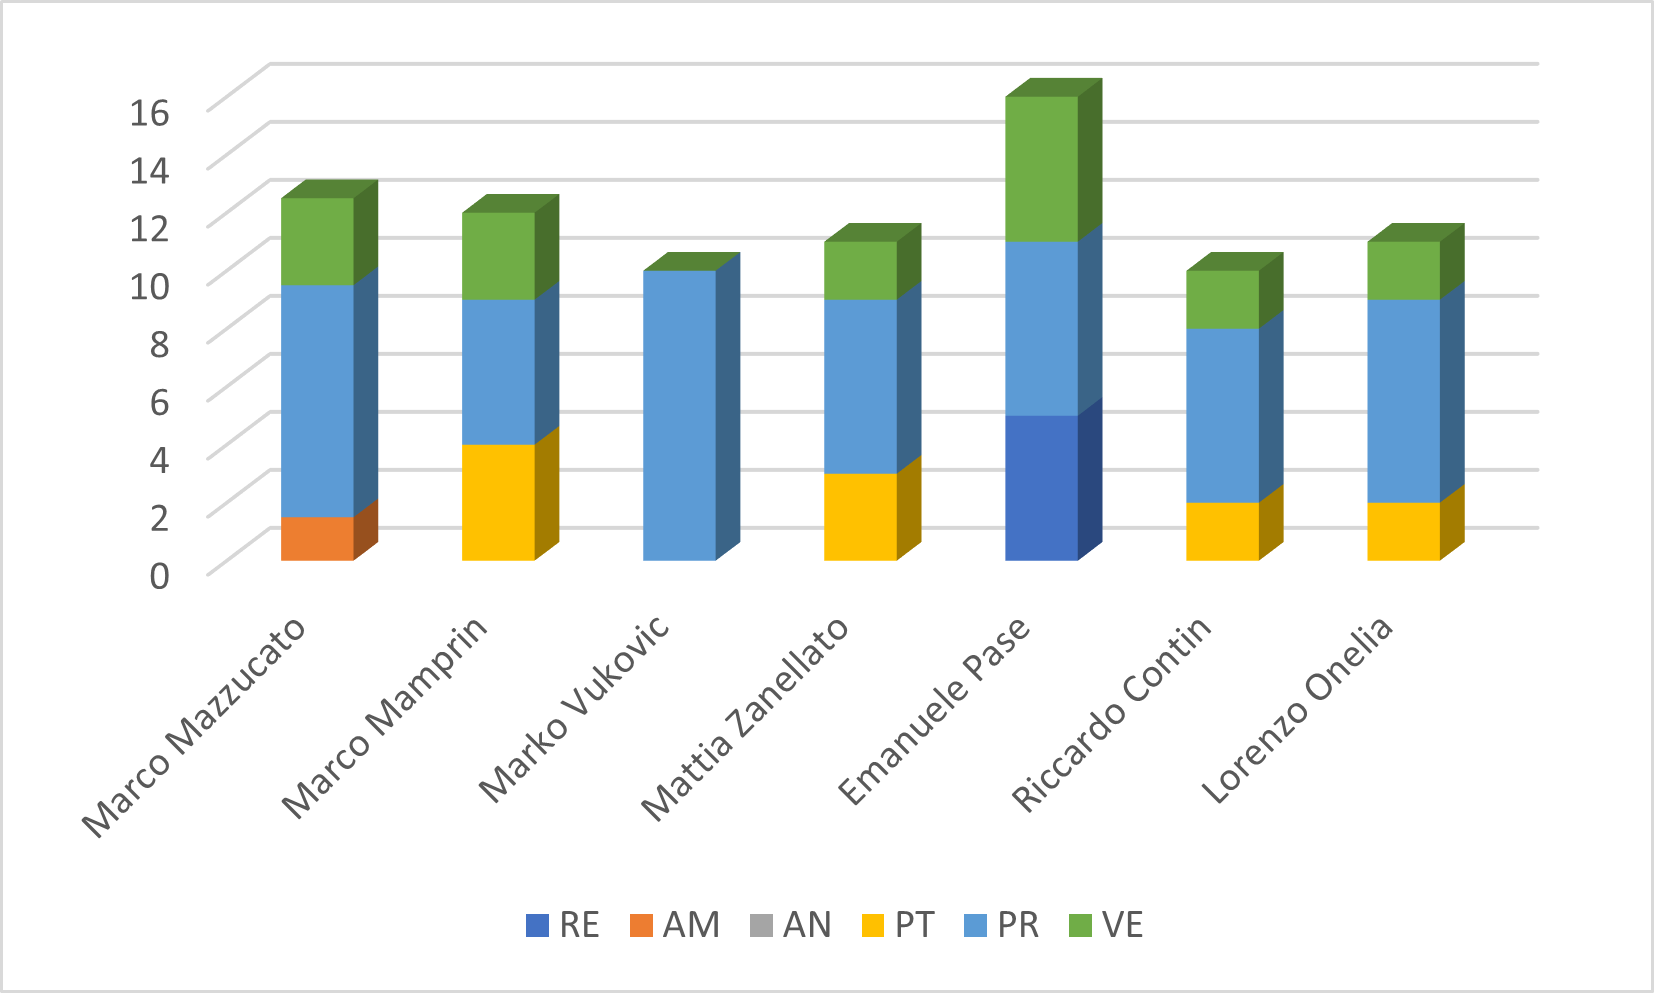
\includegraphics[width=1.0\textwidth]{Istogramma8.png}
    \caption{Istogramma della distribuzione delle ore per l'ottava milestone}
\end{figure}

\begin{figure}[H]
    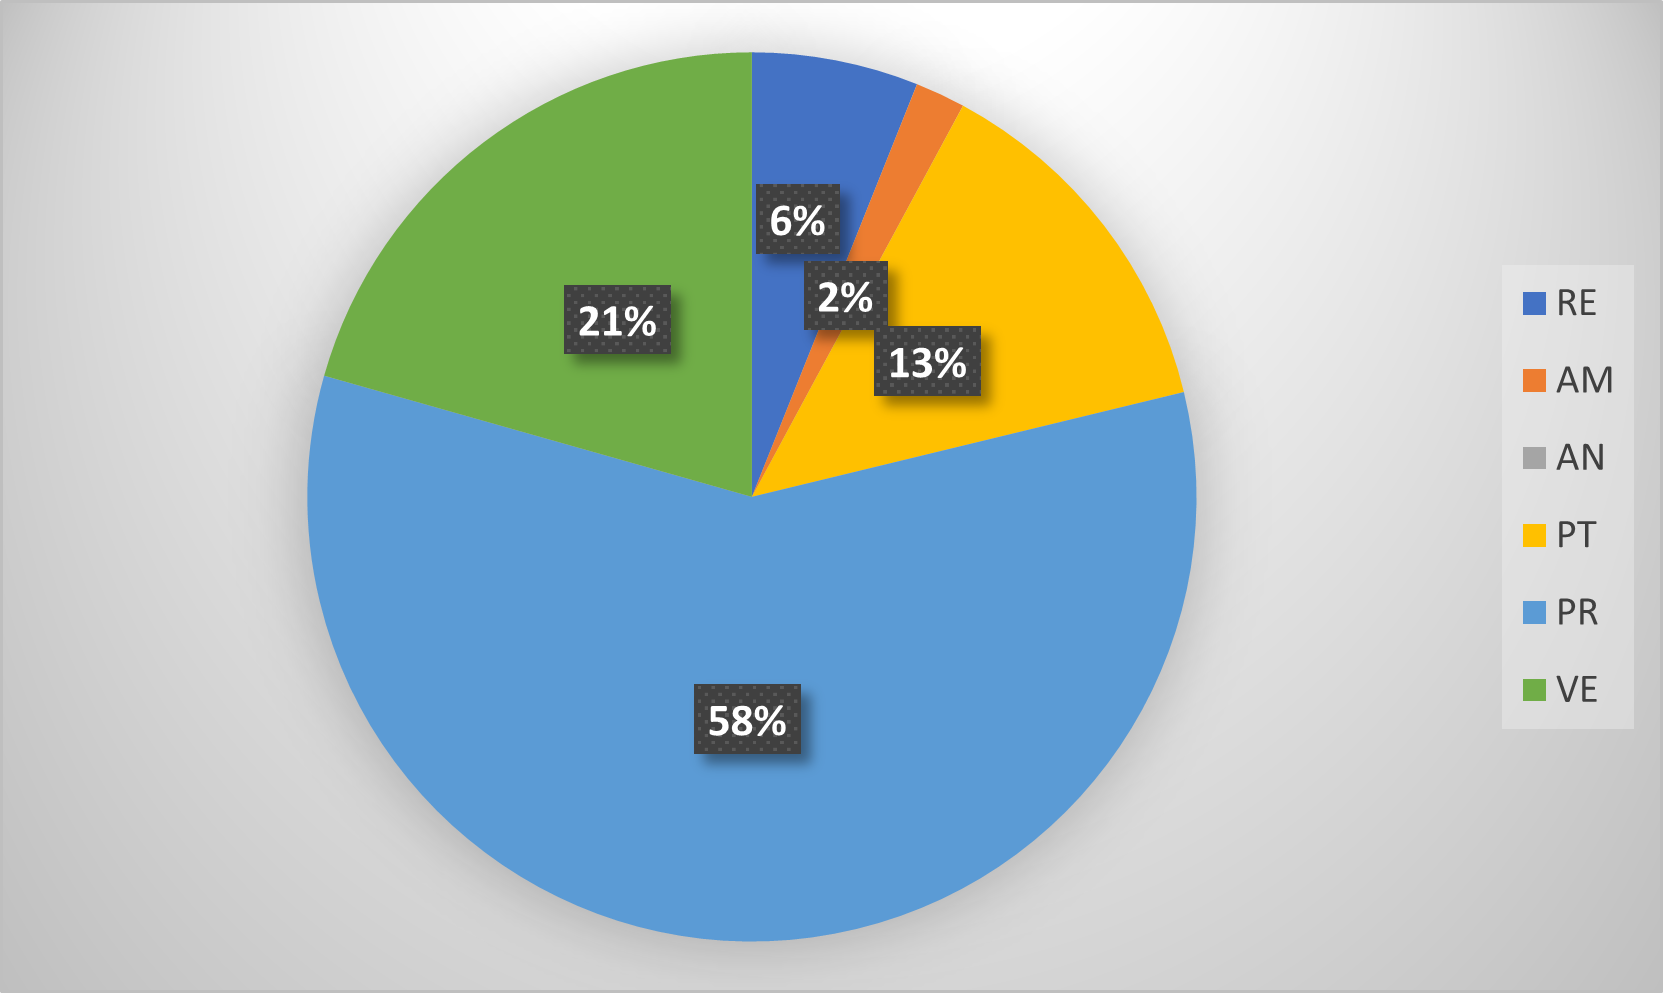
\includegraphics[width=1.0\textwidth]{Torta8.1.png}
    \caption{Grafico a torta della distribuzione delle ore per l'ottava milestone}
\end{figure}

\newpage
\subsubsection{Preventivo economico}

\begin{table}[H]
    \renewcommand\arraystretch{1.5}
    \centering
    \begin{tabular}{|l|c|c|}
    \hline
    \rowcolor[HTML]{036400}
    \textcolor{white}{\textbf{Ruolo}} & \multicolumn{1}{l|}{\textcolor{white}{\textbf{Ore}}} & \multicolumn{1}{l|}{\textcolor{white}{\textbf{Costo (€)}}} \\ \hline
    \rowcolor[HTML]{EFEFEF}\textit{Responsabile}   & 5    & 150  \\ \hline
    \rowcolor[HTML]{C0C0C0}\textit{Amministratore} & 1.5  & 30   \\ \hline
    \rowcolor[HTML]{EFEFEF}\textit{Analista}       & 0    & 0    \\ \hline
    \rowcolor[HTML]{C0C0C0}\textit{Progettista}    & 11   & 275  \\ \hline
    \rowcolor[HTML]{EFEFEF}\textit{Programmatore}  & 48   & 720  \\ \hline
    \rowcolor[HTML]{C0C0C0}\textit{Verificatore}   & 17   & 255  \\ \hline
    \rowcolor[HTML]{EFEFEF}\textbf{Totale}         & 82.5 & 1460 \\ \hline
    \end{tabular}
    \caption{Prospetto dei costi per l'ottava milestone}
\end{table}

\begin{figure}[H]
    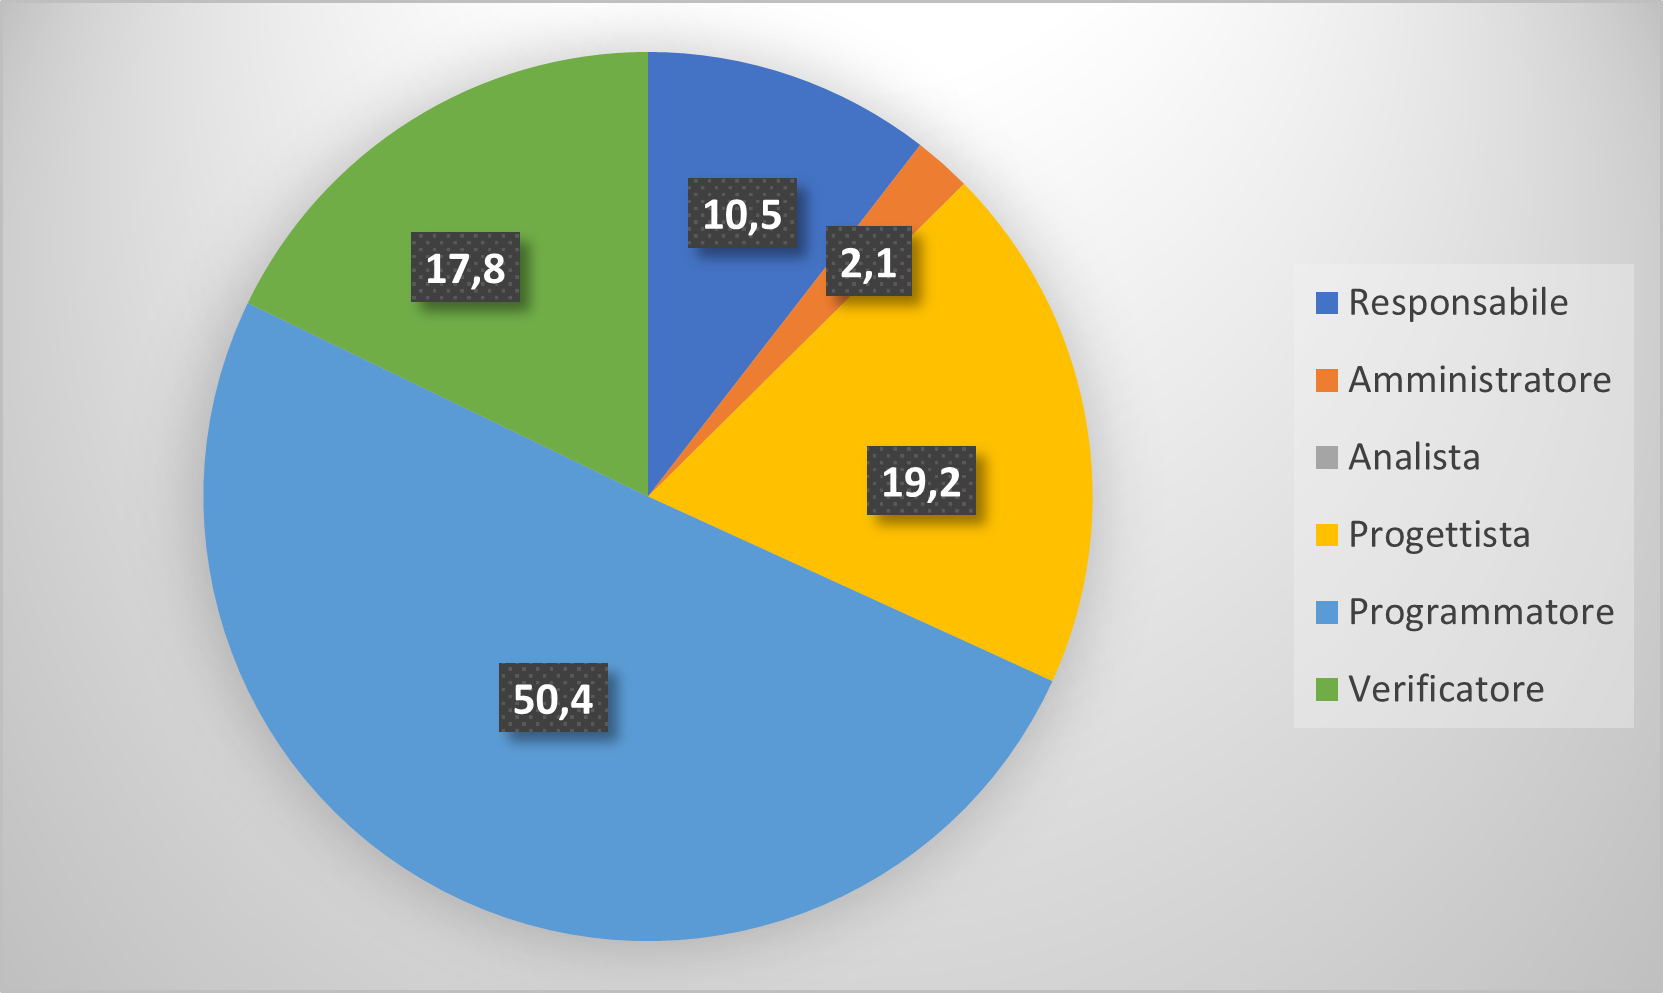
\includegraphics[width=1.0\textwidth]{Torta8.2.png}
    \caption{Grafico a torta della distribuzione dei costi per l'ottava milestone}
\end{figure}

\subsection{Nono periodo}

In questa fase i ruoli da ricoprire per portare a termine gli obiettivi pianificati sono:
\begin{itemize}
    \item \textit{Responsabile};
    \item \textit{Amministratore};
    \item \textit{Progettista};
    \item \textit{Programmatore};
    \item \textit{Verificatore}.
\end{itemize}

\subsubsection{Obiettivi}
Gli obiettivi di questo periodo sono:
\begin{itemize}
    \item Aggiornare le \textit{Norme di Progetto};
    \item Aggiornare l'\textit{Analisi dei Requisiti};
    \item Aggiornare il Cruscotto;
    \item Integrare la \textit{Specifica Architetturale};
    \item Rivedere l'architettura;
    \item Sistemare il codice già scritto;
    \item Codificare le parti mancanti;
    \item Testare il codice;
    \item Incontrare il proponente per un confronto su quanto prodotto.

\end{itemize}

\subsubsection{Preventivo orario}

\begin{table}[H]
    \renewcommand\arraystretch{1.5}
    \centering
    \begin{tabular}{|l|c|c|c|c|c|c|c|}
    \hline
    \rowcolor[HTML]{036400}
    \textcolor{white}{\textbf{Membro}} & \multicolumn{1}{l|}{\textcolor{white}{\textbf{RE}}} & \multicolumn{1}{l|}{\textcolor{white}{\textbf{AM}}} & \multicolumn{1}{l|}{\textcolor{white}{\textbf{AN}}} & \multicolumn{1}{l|}{\textcolor{white}{\textbf{PT}}} & \multicolumn{1}{l|}{\textcolor{white}{\textbf{PR}}} & \multicolumn{1}{l|}{\textcolor{white}{\textbf{VE}}} & \multicolumn{1}{l|}{\textcolor{white}{\textbf{Totale ore persona}}} \\ \hline
    \rowcolor[HTML]{EFEFEF}\textit{Marco Mazzucato}  & - & 0.5 & -  & -    & 5   & 3    & 8.5     \\ \hline
    \rowcolor[HTML]{C0C0C0}\textit{Marco Mamprin}    & - & -   & -  & 1.5  & 2   & 3.5  & 7     \\ \hline
    \rowcolor[HTML]{EFEFEF}\textit{Marko Vukovic}    & - & -   & -  & -    & -   & 5    & 5     \\ \hline
    \rowcolor[HTML]{C0C0C0}\textit{Mattia Zanellato} & - & 0.5 & -  & 1    & 3   & 3    & 7.5     \\ \hline
    \rowcolor[HTML]{EFEFEF}\textit{Emanuele Pase}    & - & -   & -  & -    & 7   & 4.5  & 11.5     \\ \hline
    \rowcolor[HTML]{C0C0C0}\textit{Riccardo Contin}  & 5 & -   & -  & 1    & 2   & 1    & 9     \\ \hline
    \rowcolor[HTML]{EFEFEF}\textit{Lorenzo Onelia}   & - & -   & -  & 1    & 7   & 2    & 10    \\ \hline
    \rowcolor[HTML]{C0C0C0}\textbf{Totale ore ruolo} & 5 & 1   & 0  & 4.5  & 26  & 22   & 58.5    \\ \hline
    \end{tabular}
    \caption{Distribuzione delle ore per la nona milestone}
\end{table}

\begin{figure}[H]
    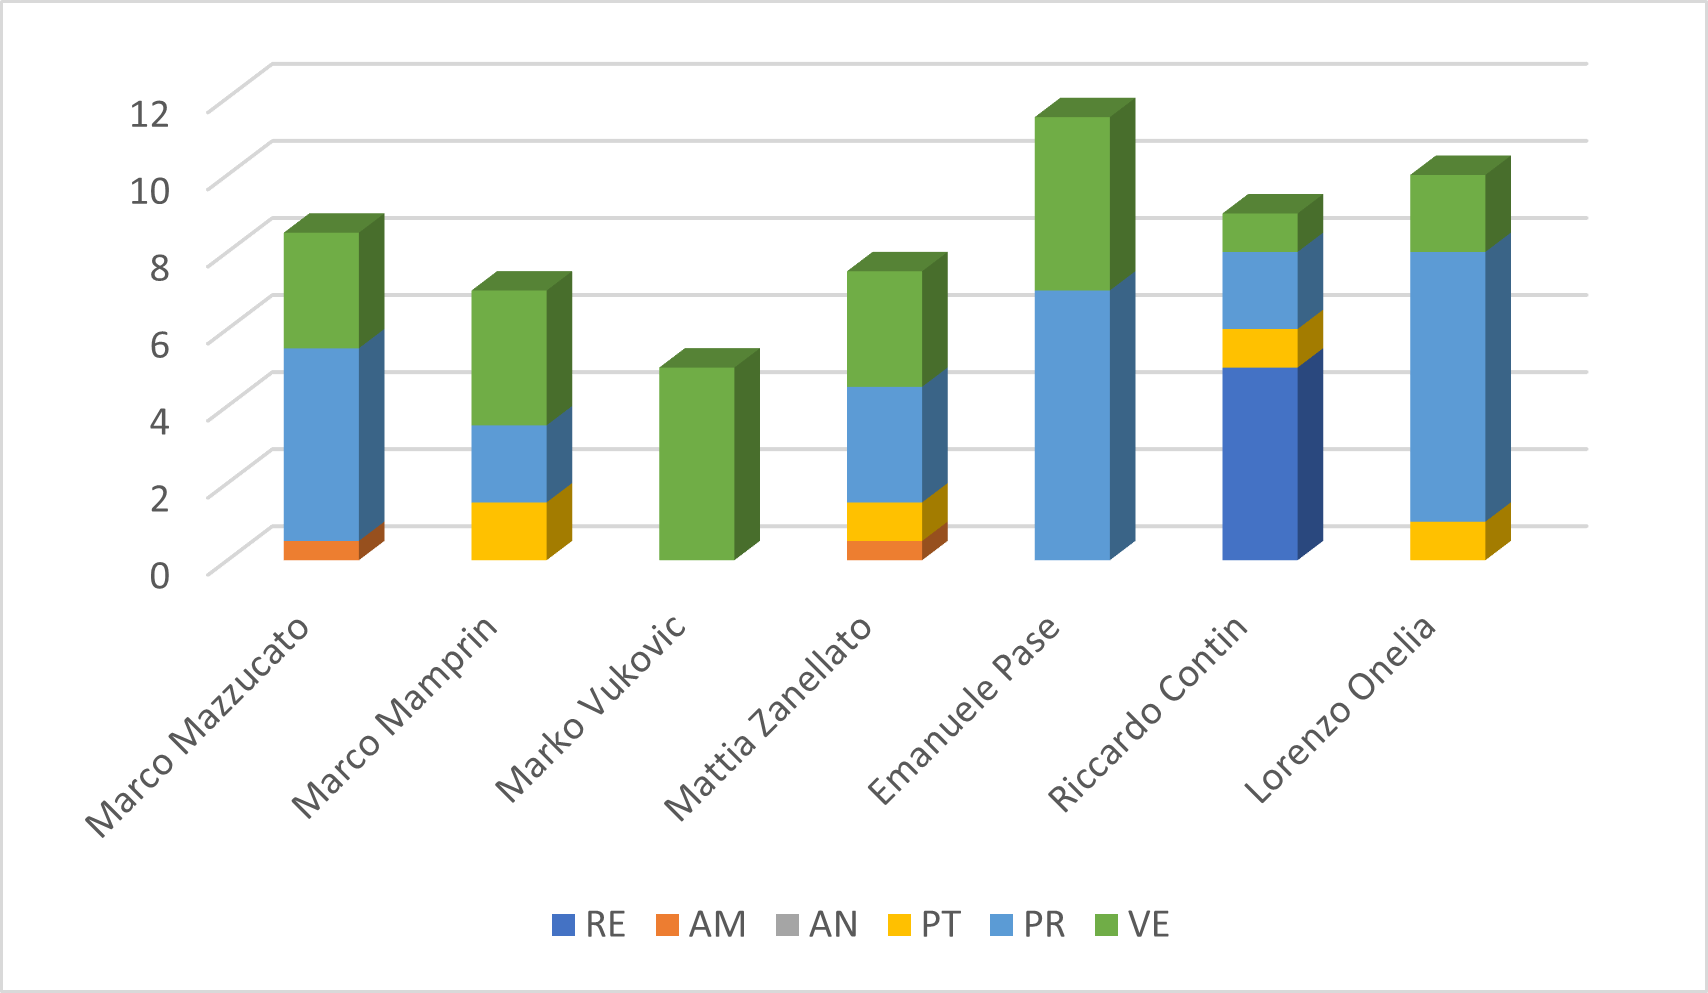
\includegraphics[width=1.0\textwidth]{Istogramma9.png}
    \caption{Istogramma della distribuzione delle ore per la nona milestone}
\end{figure}

\begin{figure}[H]
    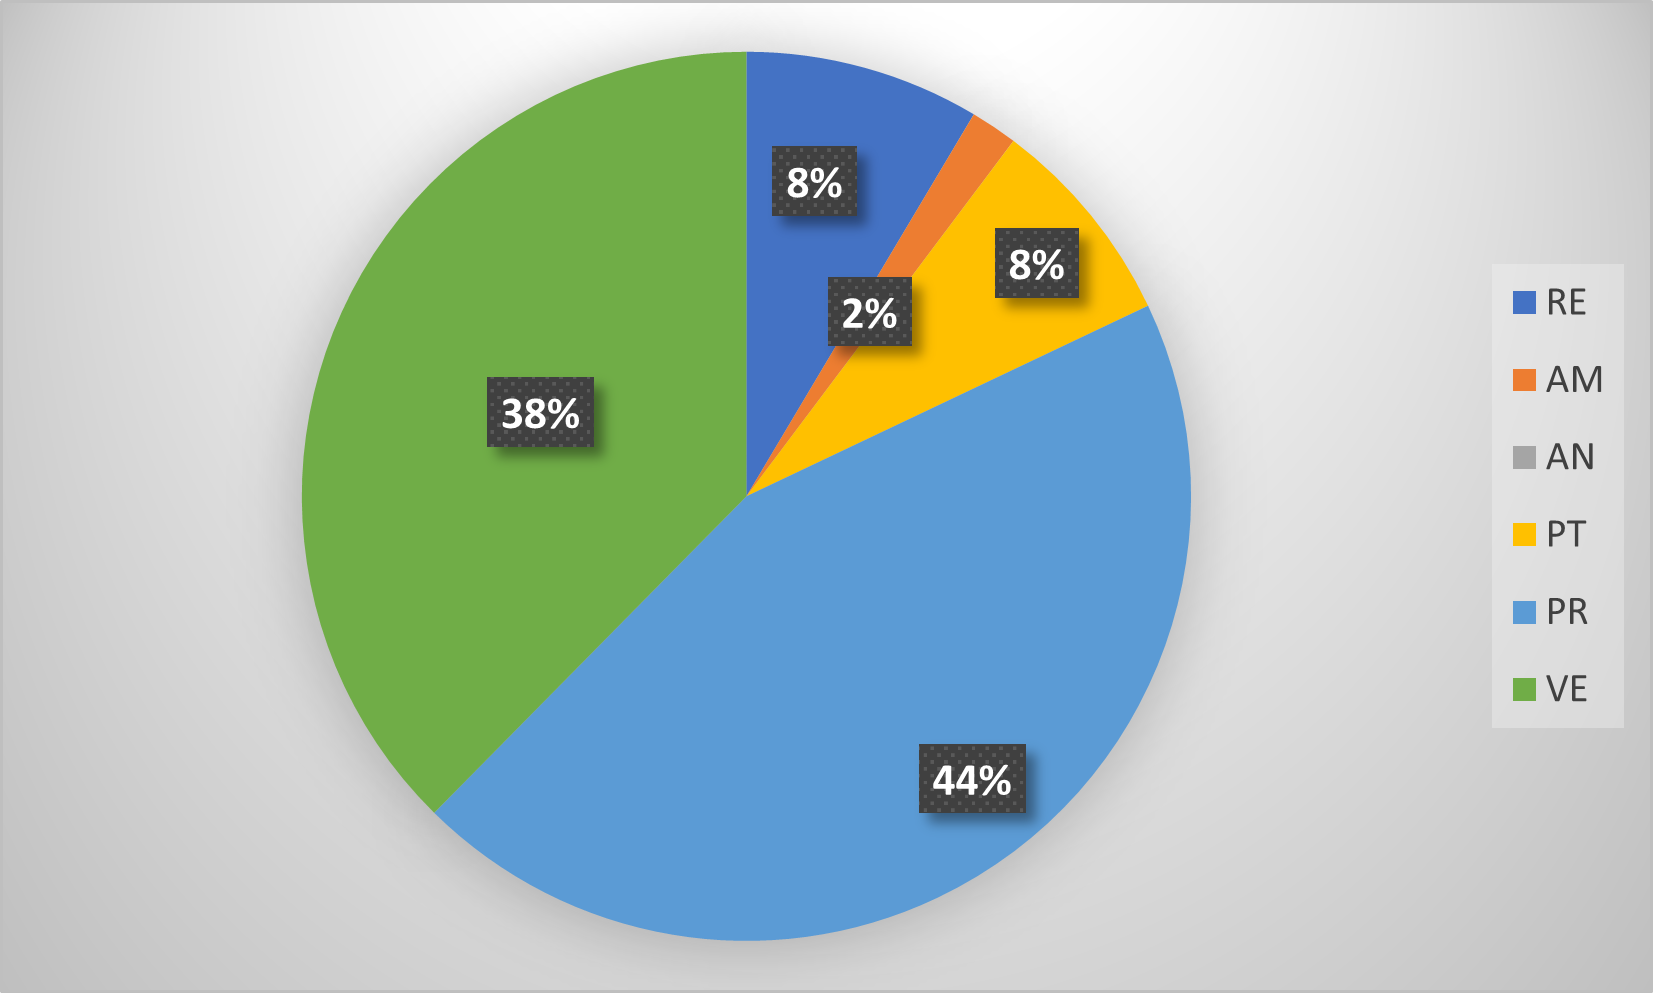
\includegraphics[width=1.0\textwidth]{Torta9.1.png}
    \caption{Grafico a torta della distribuzione delle ore per la nona milestone}
\end{figure}

\newpage
\subsubsection{Preventivo economico}

\begin{table}[H]
    \renewcommand\arraystretch{1.5}
    \centering
    \begin{tabular}{|l|c|c|}
    \hline
    \rowcolor[HTML]{036400}
    \textcolor{white}{\textbf{Ruolo}} & \multicolumn{1}{l|}{\textcolor{white}{\textbf{Ore}}} & \multicolumn{1}{l|}{\textcolor{white}{\textbf{Costo (€)}}} \\ \hline
    \rowcolor[HTML]{EFEFEF}\textit{Responsabile}   & 5    & 150    \\ \hline
    \rowcolor[HTML]{C0C0C0}\textit{Amministratore} & 1    & 20     \\ \hline
    \rowcolor[HTML]{EFEFEF}\textit{Analista}       & 0    & 0      \\ \hline
    \rowcolor[HTML]{C0C0C0}\textit{Progettista}    & 4.5  & 112.5  \\ \hline
    \rowcolor[HTML]{EFEFEF}\textit{Programmatore}  & 26   & 390    \\ \hline
    \rowcolor[HTML]{C0C0C0}\textit{Verificatore}   & 22   & 330    \\ \hline
    \rowcolor[HTML]{EFEFEF}\textbf{Totale}         & 58.5 & 1002.5 \\ \hline
    \end{tabular}
    \caption{Prospetto dei costi per la nona milestone}
\end{table}

\begin{figure}[H]
    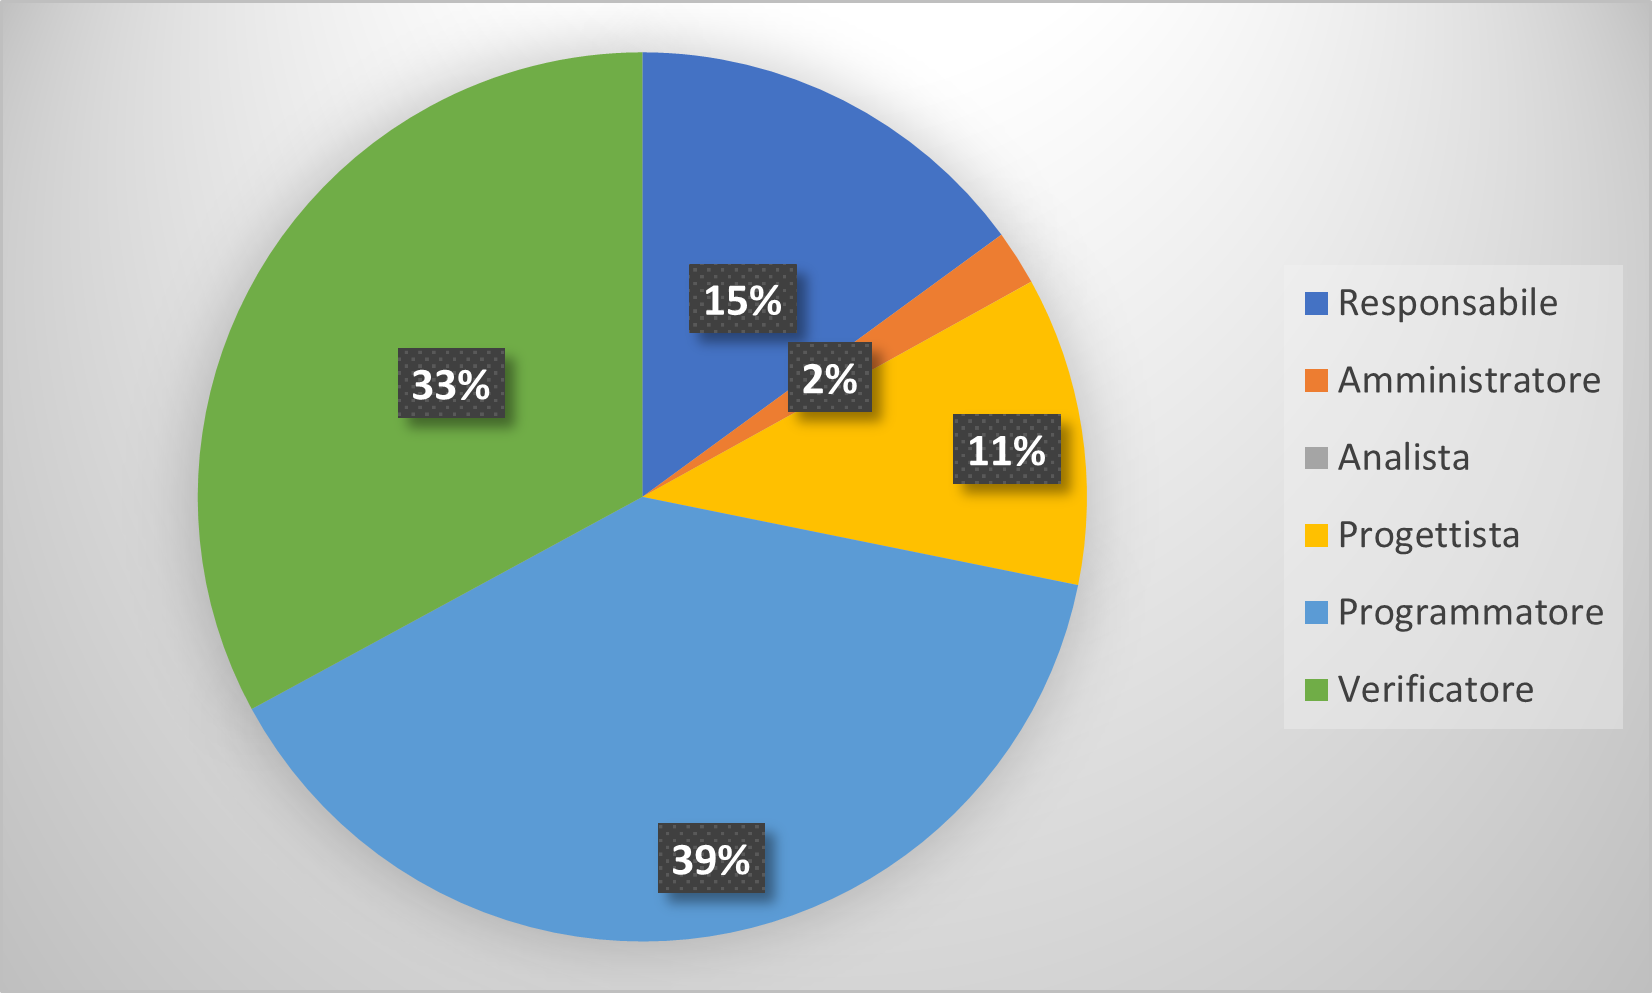
\includegraphics[width=1.0\textwidth]{Torta9.2.png}
    \caption{Grafico a torta della distribuzione dei costi per la nona milestone}
\end{figure}

\subsection{Decimo periodo}

In questa fase i ruoli da ricoprire per portare a termine gli obiettivi pianificati sono:
\begin{itemize}
    \item \textit{Responsabile};
    \item \textit{Amministratore};
    \item \textit{Progettista};
    \item \textit{Programmatore};
    \item \textit{Verificatore}.
\end{itemize}

\subsubsection{Obiettivi}
Gli obiettivi di questo periodo sono:
\begin{itemize}
    \item Terminare il documento \textit{Specifica Architetturale};
    \item Redigere la \textit{Lettera di Presentazione};
    \item Redigere il \textit{Manuale utente};
    \item Ordinare il repository  su \textbf{GitHub};
    \item Presentare la candidatura alla revisione PB.

\end{itemize}

\subsubsection{Preventivo orario}

\begin{table}[H]
    \renewcommand\arraystretch{1.5}
    \centering
    \begin{tabular}{|l|c|c|c|c|c|c|c|}
    \hline
    \rowcolor[HTML]{036400}
    \textcolor{white}{\textbf{Membro}} & \multicolumn{1}{l|}{\textcolor{white}{\textbf{RE}}} & \multicolumn{1}{l|}{\textcolor{white}{\textbf{AM}}} & \multicolumn{1}{l|}{\textcolor{white}{\textbf{AN}}} & \multicolumn{1}{l|}{\textcolor{white}{\textbf{PT}}} & \multicolumn{1}{l|}{\textcolor{white}{\textbf{PR}}} & \multicolumn{1}{l|}{\textcolor{white}{\textbf{VE}}} & \multicolumn{1}{l|}{\textcolor{white}{\textbf{Totale ore persona}}} \\ \hline
    \rowcolor[HTML]{EFEFEF}\textit{Marco Mazzucato}  & - & -   & -  & -    & 5   & 1    & 6     \\ \hline
    \rowcolor[HTML]{C0C0C0}\textit{Marco Mamprin}    & - & 0.5 & -  & 1    & -   & 2    & 3.5     \\ \hline
    \rowcolor[HTML]{EFEFEF}\textit{Marko Vukovic}    & - & -   & -  & -    & -   & -    & -     \\ \hline
    \rowcolor[HTML]{C0C0C0}\textit{Mattia Zanellato} & 4 & -   & -  & -    & -   & 2    & 6     \\ \hline
    \rowcolor[HTML]{EFEFEF}\textit{Emanuele Pase}    & - & -   & -  & -    & 2.5 & 2.5  & 5     \\ \hline
    \rowcolor[HTML]{C0C0C0}\textit{Riccardo Contin}  & - & -   & -  & -    & 1   & 2    & 3     \\ \hline
    \rowcolor[HTML]{EFEFEF}\textit{Lorenzo Onelia}   & - & -   & -  & -    & 2.5 & 2.5  & 5    \\ \hline
    \rowcolor[HTML]{C0C0C0}\textbf{Totale ore ruolo} & 4 & 0.5 & 0  & 1    & 11  & 12   & 28.5    \\ \hline
    \end{tabular}
    \caption{Distribuzione delle ore per la decima milestone}
\end{table}

\begin{figure}[H]
    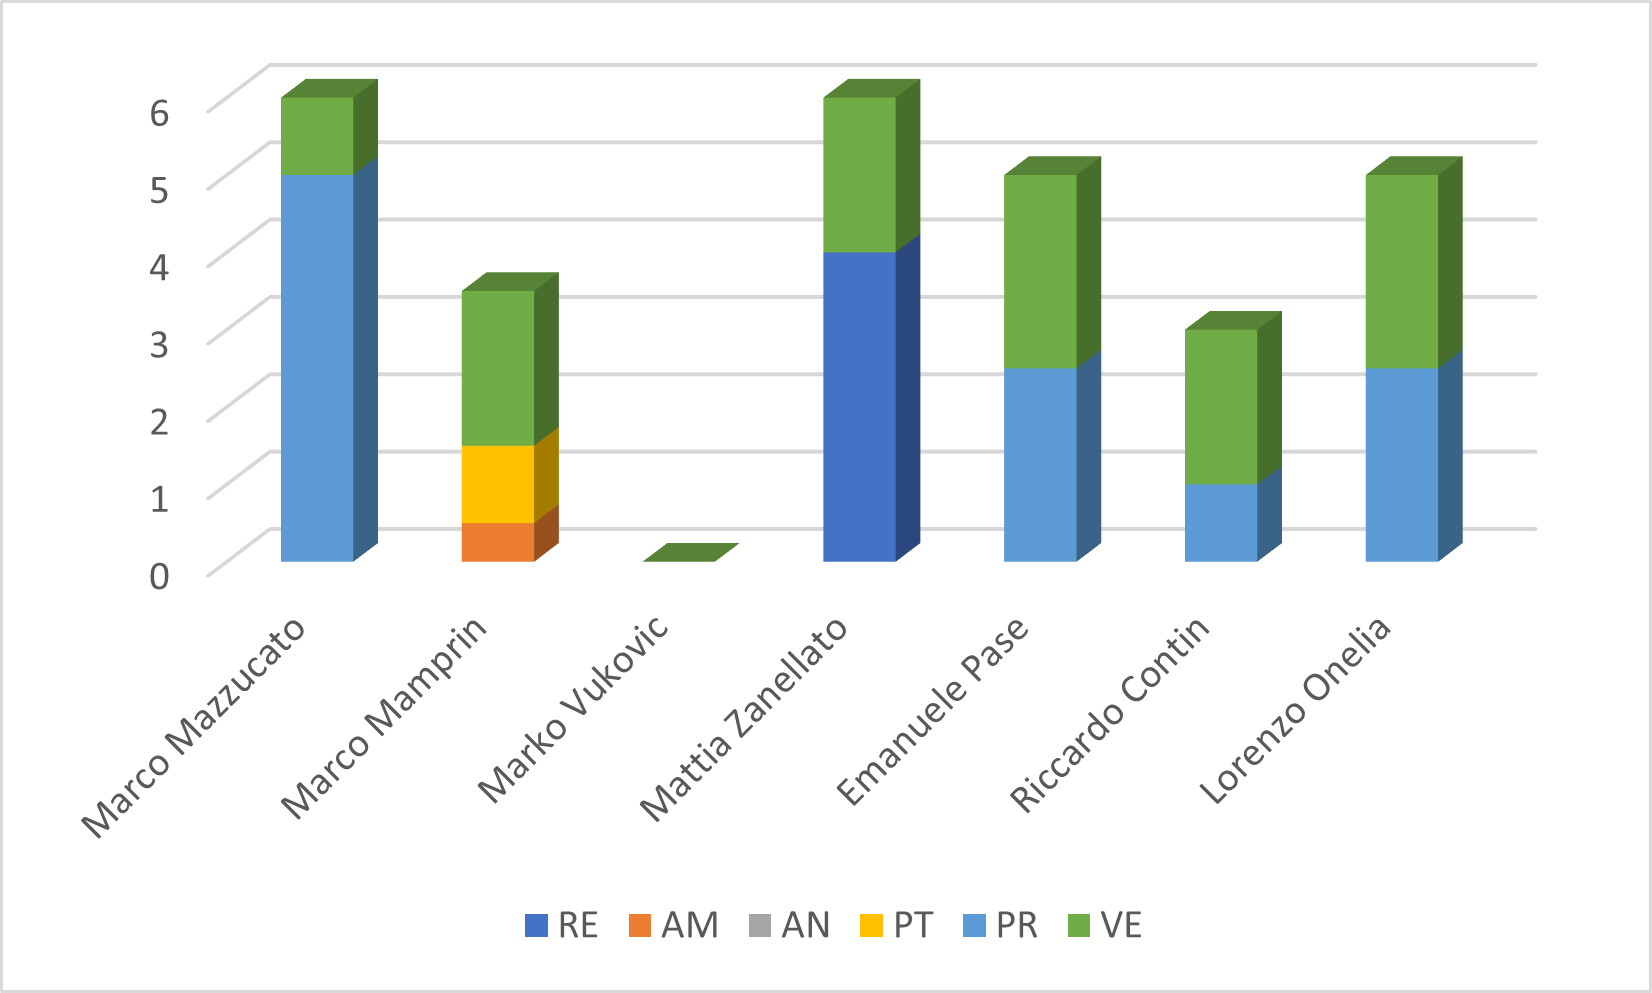
\includegraphics[width=1.0\textwidth]{Istogramma10.png}
    \caption{Istogramma della distribuzione delle ore per la decima milestone}
\end{figure}

\begin{figure}[H]
    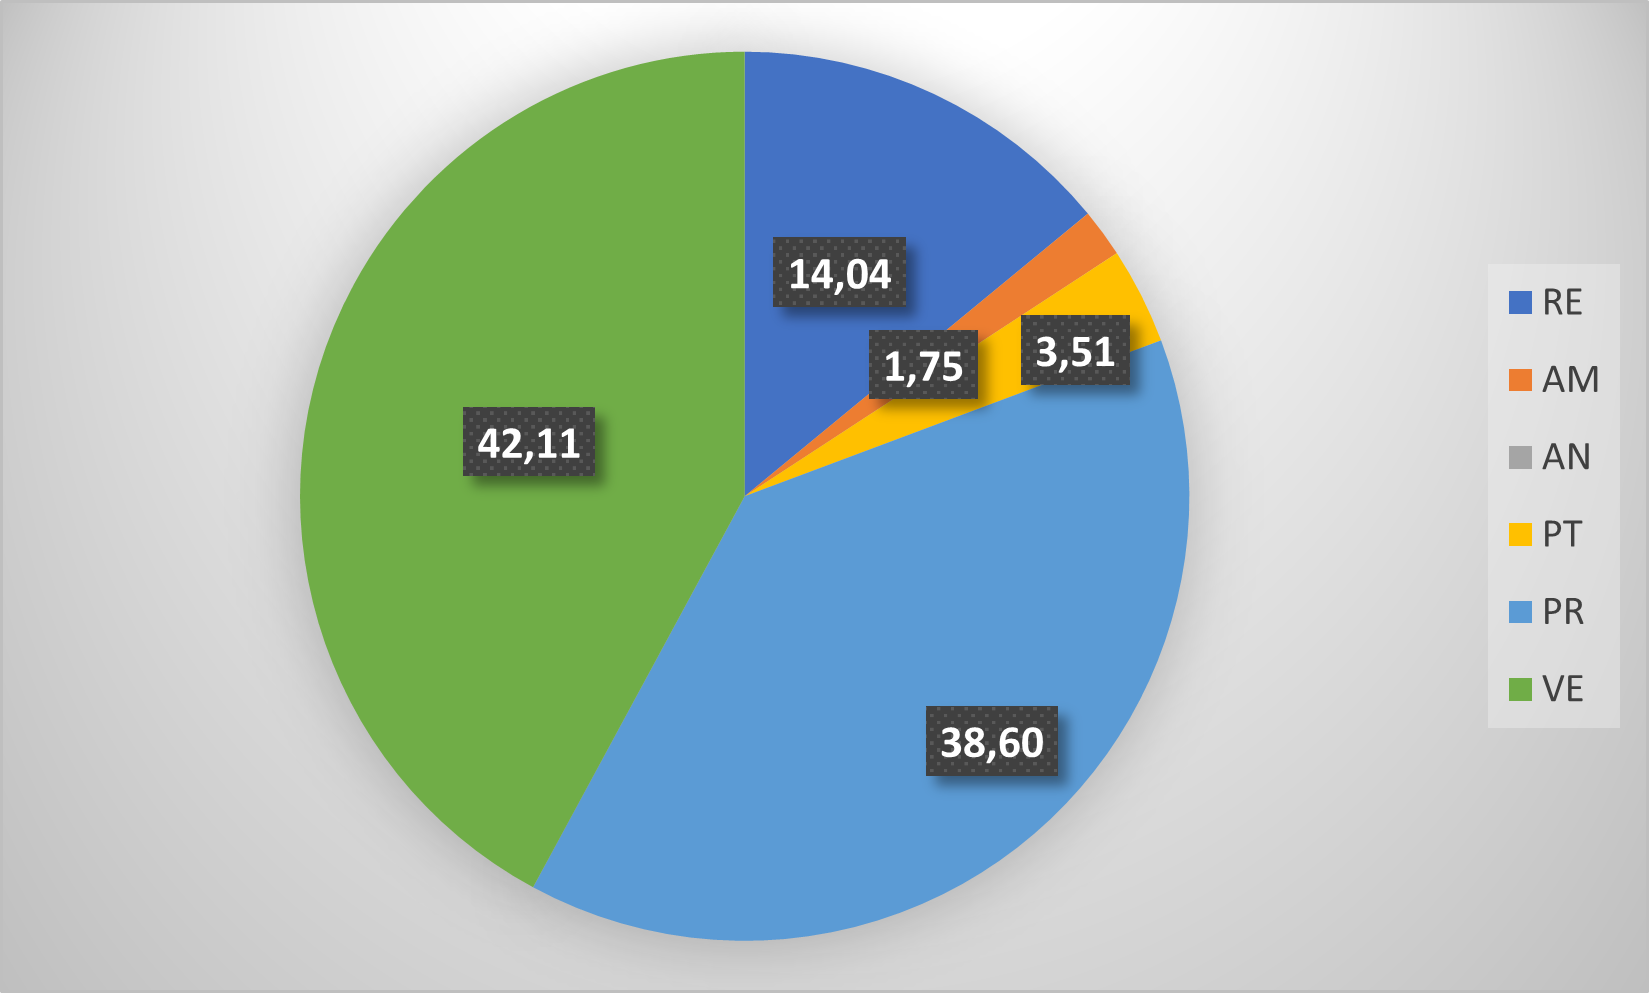
\includegraphics[width=1.0\textwidth]{Torta10.1.png}
    \caption{Grafico a torta della distribuzione delle ore per la decima milestone}
\end{figure}

\newpage
\subsubsection{Preventivo economico}

\begin{table}[H]
    \renewcommand\arraystretch{1.5}
    \centering
    \begin{tabular}{|l|c|c|}
    \hline
    \rowcolor[HTML]{036400}
    \textcolor{white}{\textbf{Ruolo}} & \multicolumn{1}{l|}{\textcolor{white}{\textbf{Ore}}} & \multicolumn{1}{l|}{\textcolor{white}{\textbf{Costo (€)}}} \\ \hline
    \rowcolor[HTML]{EFEFEF}\textit{Responsabile}   & 4    & 120    \\ \hline
    \rowcolor[HTML]{C0C0C0}\textit{Amministratore} & 0.5  & 10     \\ \hline
    \rowcolor[HTML]{EFEFEF}\textit{Analista}       & 0    & 0      \\ \hline
    \rowcolor[HTML]{C0C0C0}\textit{Progettista}    & 1    & 25     \\ \hline
    \rowcolor[HTML]{EFEFEF}\textit{Programmatore}  & 11   & 165    \\ \hline
    \rowcolor[HTML]{C0C0C0}\textit{Verificatore}   & 12   & 180    \\ \hline
    \rowcolor[HTML]{EFEFEF}\textbf{Totale}         & 28.5 & 500    \\ \hline
    \end{tabular}
    \caption{Prospetto dei costi per la decima milestone}
\end{table}

\begin{figure}[H]
    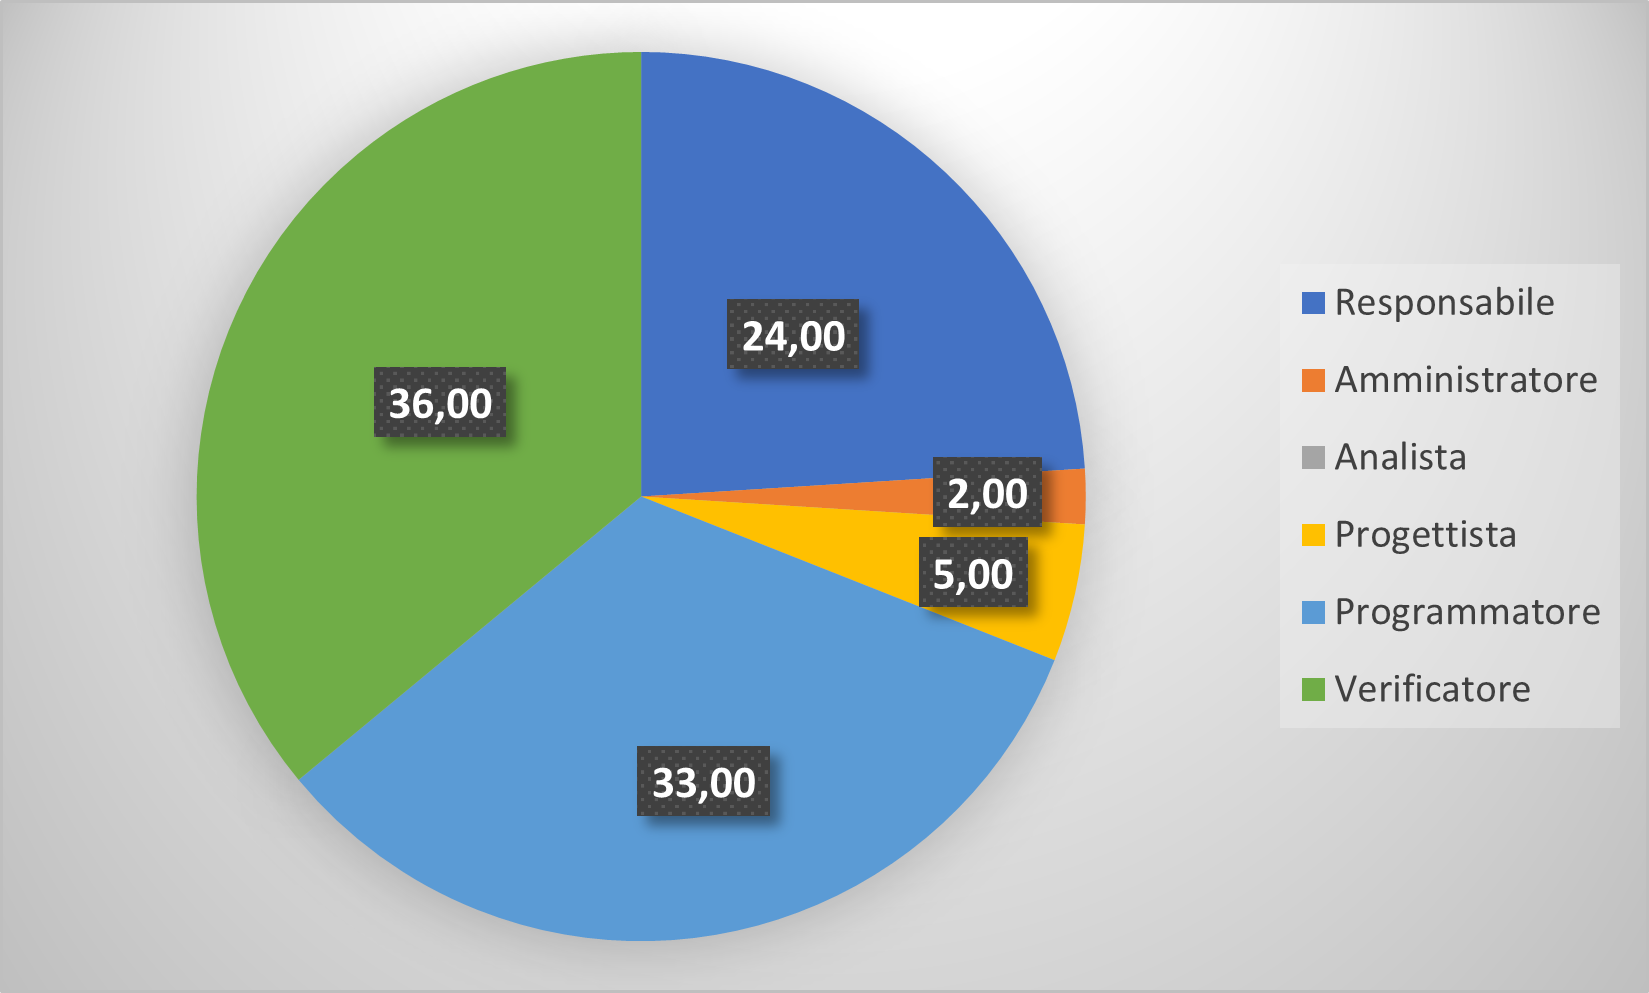
\includegraphics[width=1.0\textwidth]{Torta10.2.png}
    \caption{Grafico a torta della distribuzione dei costi per la decima milestone}
\end{figure}



\newpage
\section{Verso la CA}

\subsection{Undicesimo periodo}

In questa fase i ruoli da ricoprire per portare a termine gli obiettivi pianificati sono:
\begin{itemize}
    \item \textit{Responsabile};
    \item \textit{Progettista};
    \item \textit{Programmatore};
    \item \textit{Verificatore}.
\end{itemize}

\subsubsection{Obiettivi}
Gli obiettivi di questo periodo sono:
\begin{itemize}
    \item Risolvere il baco nello Scatter Plot 2;
    \item Redarre il \textit{Manuale Sviluppatore};
    \item Ultimare lo unit testing;
    \item Implementare il grafico Force Directed Graph;
    \item Implementare i feedback per l'utente al prodotto.

\end{itemize}

\subsubsection{Preventivo orario}

\begin{table}[H]
    \renewcommand\arraystretch{1.5}
    \centering
    \begin{tabular}{|l|c|c|c|c|c|c|c|}
    \hline
    \rowcolor[HTML]{036400}
    \textcolor{white}{\textbf{Membro}} & \multicolumn{1}{l|}{\textcolor{white}{\textbf{RE}}} & \multicolumn{1}{l|}{\textcolor{white}{\textbf{AM}}} & \multicolumn{1}{l|}{\textcolor{white}{\textbf{AN}}} & \multicolumn{1}{l|}{\textcolor{white}{\textbf{PT}}} & \multicolumn{1}{l|}{\textcolor{white}{\textbf{PR}}} & \multicolumn{1}{l|}{\textcolor{white}{\textbf{VE}}} & \multicolumn{1}{l|}{\textcolor{white}{\textbf{Totale ore persona}}} \\ \hline
    \rowcolor[HTML]{EFEFEF}\textit{Marco Mazzucato}  & -   & -   & -  & -    & 1    & 4      & 5     \\ \hline
    \rowcolor[HTML]{C0C0C0}\textit{Marco Mamprin}    & -   & -   & -  & 1    & 2    & 1      & 4     \\ \hline
    \rowcolor[HTML]{EFEFEF}\textit{Marko Vukovic}    & -   & -   & -  & -    & -    & -      & -     \\ \hline
    \rowcolor[HTML]{C0C0C0}\textit{Mattia Zanellato} & -   & -   & -  & -    & 1    & 2      & 3     \\ \hline
    \rowcolor[HTML]{EFEFEF}\textit{Emanuele Pase}    & -   & -   & -  & -    & 1.5  & 2.5    & 4     \\ \hline
    \rowcolor[HTML]{C0C0C0}\textit{Riccardo Contin}  & -   & -   & -  & -    & 3    & 4      & 7     \\ \hline
    \rowcolor[HTML]{EFEFEF}\textit{Lorenzo Onelia}   & 4.5 & -   & -  & -    & -    & 1      & 5.5    \\ \hline
    \rowcolor[HTML]{C0C0C0}\textbf{Totale ore ruolo} & 4.5 & 0   & 0  & 1    & 8.5  & 14.5   & 28.5    \\ \hline
    \end{tabular}
    \caption{Distribuzione delle ore per la undicesima milestone}
\end{table}

\begin{figure}[H]
    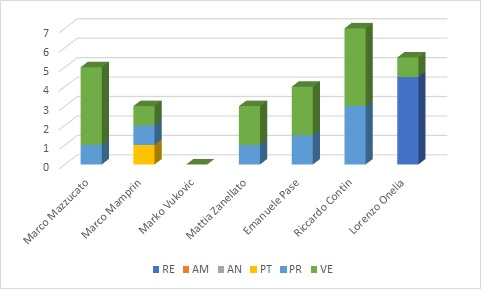
\includegraphics[width=1.0\textwidth]{Istogramma11.jpg}
    \caption{Istogramma della distribuzione delle ore per la undicesima milestone}
\end{figure}

\begin{figure}[H]
    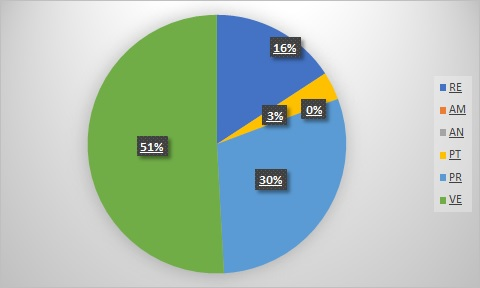
\includegraphics[width=1.0\textwidth]{Torta11.1.jpg}
    \caption{Grafico a torta della distribuzione delle ore per la undicesima milestone}
\end{figure}

\newpage
\subsubsection{Preventivo economico}

\begin{table}[H]
    \renewcommand\arraystretch{1.5}
    \centering
    \begin{tabular}{|l|c|c|}
    \hline
    \rowcolor[HTML]{036400}
    \textcolor{white}{\textbf{Ruolo}} & \multicolumn{1}{l|}{\textcolor{white}{\textbf{Ore}}} & \multicolumn{1}{l|}{\textcolor{white}{\textbf{Costo (€)}}} \\ \hline
    \rowcolor[HTML]{EFEFEF}\textit{Responsabile}   & 4.5    & 135    \\ \hline
    \rowcolor[HTML]{C0C0C0}\textit{Amministratore} & 0  & 0     \\ \hline
    \rowcolor[HTML]{EFEFEF}\textit{Analista}       & 0    & 0      \\ \hline
    \rowcolor[HTML]{C0C0C0}\textit{Progettista}    & 1    & 25     \\ \hline
    \rowcolor[HTML]{EFEFEF}\textit{Programmatore}  & 8.5   & 127.5    \\ \hline
    \rowcolor[HTML]{C0C0C0}\textit{Verificatore}   & 14.5   & 217.5    \\ \hline
    \rowcolor[HTML]{EFEFEF}\textbf{Totale}         & 28.5 & 505    \\ \hline
    \end{tabular}
    \caption{Prospetto dei costi per la undicesima milestone}
\end{table}

\begin{figure}[H]
    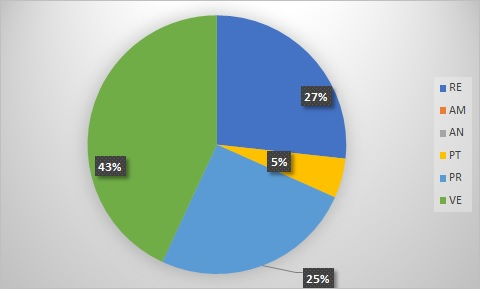
\includegraphics[width=1.0\textwidth]{Torta11.2.jpg}
    \caption{Grafico a torta della distribuzione dei costi per la undicesima milestone}
\end{figure}

  \chapter{Consuntivo}
\renewcommand\arraystretch{1,2}

Nel consuntivo$_G$, vengono riprese le tabelle del preventivo. Al posto dei valori inseriti nel preventivo, si inserisce:
\begin{itemize}
    \item Valore effettivo consuntivato;
    \item Se il valore precedente è diverso da quello del preventivo$_G$, due parentesi tonde con all'interno
        la differenza tra valore di consuntivo e valore di preventivo.
\end{itemize}

\section{Verso la RTB}

\subsection{Primo periodo}


\subsubsection{Consuntivo orario}
\begin{table}[H]
    \renewcommand\arraystretch{1.5}
    \centering
    \begin{adjustwidth}{-1.15cm}{}
    \begin{tabular}{|l|c|c|c|c|c|c|c|}
    \hline
    \rowcolor[HTML]{036400}
    \textcolor{white}{\textbf{Membro}} & \multicolumn{1}{c|}{\textcolor{white}{\textbf{RE}}} & \multicolumn{1}{c|}{\textcolor{white}{\textbf{AM}}} & \multicolumn{1}{c|}{\textcolor{white}{\textbf{AN}}} & \multicolumn{1}{c|}{\textcolor{white}{\textbf{PT}}} & \multicolumn{1}{c|}{\textcolor{white}{\textbf{PR}}} & \multicolumn{1}{c|}{\textcolor{white}{\textbf{VE}}} & \multicolumn{1}{c|}{\textcolor{white}{\textbf{Totale ore persona}}} \\ \hline
    \rowcolor[HTML]{EFEFEF}\textit{Marco Mazzucato}  & 3 (+1) & 3          & - & - & - & 1         & 7 (+1)   \\ \hline
    \rowcolor[HTML]{C0C0C0}\textit{Marco Mamprin}    & -      & 2 (-1)     & - & - & - & 1.5 (+0.5)& 3.5 (-0.5) \\ \hline
    \rowcolor[HTML]{EFEFEF}\textit{Marko Vukovic}    & 2      & 3          & - & - & - & 1         & 6        \\ \hline
    \rowcolor[HTML]{C0C0C0}\textit{Mattia Zanellato} & -      & 1.5 (-1.5) & - & - & - & 2.5 (+1.5)& 4        \\ \hline
    \rowcolor[HTML]{EFEFEF}\textit{Emanuele Pase}    & -      & 2.5 (-0.5) & - & - & - & 1         & 3.5 (-0.5) \\ \hline
    \rowcolor[HTML]{C0C0C0}\textit{Riccardo Contin}  & -      & 3          & - & - & - & 1         & 4        \\ \hline
    \rowcolor[HTML]{EFEFEF}\textit{Lorenzo Onelia}   & -      & 2.5 (-0.5) & - & - & - & 2 (+1)    & 4.5 (+0.5) \\ \hline
    \rowcolor[HTML]{C0C0C0}\textbf{Totale ore ruolo} & 5 (+1) & 17.5 (-3.5)& - & - & - & 10 (+3)   & 32.5 (+0.5)\\ \hline
    \end{tabular}
    \end{adjustwidth}
    \caption{Distribuzione delle ore per la prima milestone}
\end{table}


\begin{table}[H]
    \renewcommand\arraystretch{1.5}
    \centering
    \begin{tabular}{|l|c|c|c|c|c|c|c|}
    \hline
    \rowcolor[HTML]{036400}
    \textcolor{white}{\textbf{Membro}} & \multicolumn{1}{c|}{\textcolor{white}{\textbf{RE}}} & \multicolumn{1}{c|}{\textcolor{white}{\textbf{AM}}} & \multicolumn{1}{c|}{\textcolor{white}{\textbf{AN}}} & \multicolumn{1}{c|}{\textcolor{white}{\textbf{PT}}} & \multicolumn{1}{c|}{\textcolor{white}{\textbf{PR}}} & \multicolumn{1}{c|}{\textcolor{white}{\textbf{VE}}} & \multicolumn{1}{c|}{\textcolor{white}{\textbf{Totale ore persona}}} \\ \hline
    \rowcolor[HTML]{EFEFEF}\textit{Marco Mazzucato}  & 6  & 5   & 5  & 23  & 24 & 25   & 88   \\ \hline
    \rowcolor[HTML]{C0C0C0}\textit{Marco Mamprin}    & 9  & 6   & 5  & 23  & 24 & 24.5 & 91.5 \\ \hline
    \rowcolor[HTML]{EFEFEF}\textit{Marko Vukovic}    & 7  & 5   & 5  & 23  & 24 & 25   & 89   \\ \hline
    \rowcolor[HTML]{C0C0C0}\textit{Mattia Zanellato} & 9  & 6.5 & 5  & 23  & 24 & 23.5 & 91   \\ \hline
    \rowcolor[HTML]{EFEFEF}\textit{Emanuele Pase}    & 9  & 5.5 & 5  & 23  & 24 & 25   & 91.5 \\ \hline
    \rowcolor[HTML]{C0C0C0}\textit{Riccardo Contin}  & 9  & 5   & 5  & 23  & 24 & 25   & 91   \\ \hline
    \rowcolor[HTML]{EFEFEF}\textit{Lorenzo Onelia}   & 9  & 5.5 & 5  & 23  & 24 & 24   & 90.5 \\ \hline
    \textbf{Totale ore ruolo} & 58 & 38.5& 35 & 161 & 168& 172  & 632.5\\ \hline
    \end{tabular}
    \caption{Ore rimaste dopo la prima milestone}
\end{table}

\subsubsection{Consuntivo economico}

\begin{table}[H]
    \renewcommand\arraystretch{1.5}
    \centering
    \begin{tabular}{|l|c|c|}
    \hline
    \rowcolor[HTML]{036400}
    \textcolor{white}{\textbf{Ruolo}} & \multicolumn{1}{l|}{\textcolor{white}{\textbf{Ore}}} & \multicolumn{1}{l|}{\textcolor{white}{\textbf{Costo (€)}}} \\ \hline
    \rowcolor[HTML]{EFEFEF}\textit{Responsabile}      & 5 (+1)    & 150 (+30) \\ \hline
    \rowcolor[HTML]{C0C0C0}\textit{Amministratore}    & 17.5 (-3.5) & 350 (-70) \\ \hline
    \rowcolor[HTML]{EFEFEF}\textit{Analista}          & -         & -         \\ \hline
    \rowcolor[HTML]{C0C0C0}\textit{Progettista}       & -         & -         \\ \hline
    \rowcolor[HTML]{EFEFEF}\textit{Programmatore}     & -         & -         \\ \hline
    \rowcolor[HTML]{C0C0C0}\textit{Verificatore}      & 10 (+3)    & 150 (+45) \\ \hline
    \rowcolor[HTML]{EFEFEF}\textbf{Totale Preventivo} & 32        & 645       \\ \hline
    \rowcolor[HTML]{C0C0C0}\textbf{Totale Consuntivo} & 32.5      & 650       \\ \hline
    \rowcolor[HTML]{EFEFEF}\textbf{Differenza}        & +0.5      & +5       \\ \hline
    \end{tabular}
    \caption{Consuntivo dei costi per la prima milestone}
\end{table}

\subsubsection{Conclusioni}
Dal consuntivo si può dedurre che il gruppo è stato quasi in linea con il preventivo di periodo.
L'unica differenza è stata che sono servite meno ore di \textit{Amministratore} e più
ore di \textit{Responsabile} e \textit{Verificatore}. Questo ha portato a una spesa maggiore di 5€ per un
complessivo di 650€ a fronte dei 645€ previsti.
In conclusione il budget rimanente è di \num{12510}€.



\subsection{Secondo periodo}

\subsubsection{Consuntivo orario}
\begin{table}[H]
    \renewcommand\arraystretch{1.5}
    \centering
    \begin{adjustwidth}{-1.25cm}{}
    \begin{tabular}{|l|c|c|c|c|c|c|c|}
    \hline
    \rowcolor[HTML]{036400}
    \textcolor{white}{\textbf{Membro}} & \multicolumn{1}{c|}{\textcolor{white}{\textbf{RE}}} & \multicolumn{1}{c|}{\textcolor{white}{\textbf{AM}}} & \multicolumn{1}{c|}{\textcolor{white}{\textbf{AN}}} & \multicolumn{1}{c|}{\textcolor{white}{\textbf{PT}}} & \multicolumn{1}{c|}{\textcolor{white}{\textbf{PR}}} & \multicolumn{1}{c|}{\textcolor{white}{\textbf{VE}}} & \multicolumn{1}{c|}{\textcolor{white}{\textbf{Totale ore persona}}} \\ \hline
    \rowcolor[HTML]{EFEFEF}\textit{Marco Mazzucato}  & -      & 2            & 2          & - & - & 1 (-1)        & 5 (-1)         \\ \hline
    \rowcolor[HTML]{C0C0C0}\textit{Marco Mamprin}    & -      & 2            & 0.5 (-0.5)   & - & - & 1 (-1)        & 3.5 (-1.5)       \\ \hline
    \rowcolor[HTML]{EFEFEF}\textit{Marko Vukovic}    & -      & 1.5          & 2 (-1)     & - & - & 3             & 6.5 (-1)       \\ \hline
    \rowcolor[HTML]{C0C0C0}\textit{Mattia Zanellato} & -      & -            & 3          & - & - & 2.5 (-0.5)      & 5.5 (-0.5)       \\ \hline
    \rowcolor[HTML]{EFEFEF}\textit{Emanuele Pase}    & -      & -            & 3          & - & - & 2.5 (-0.5)      & 5.5 (-0.5)       \\ \hline
    \rowcolor[HTML]{C0C0C0}\textit{Riccardo Contin}  & 4      & -            & 2 (-1)     & - & - & 1.5 (+0.5)      & 7.5 (-0.5)       \\ \hline
    \rowcolor[HTML]{EFEFEF}\textit{Lorenzo Onelia}   & -      & 0 (-2)       & 1 (-1)     & - & - & 3.5 (+0.5)      & 4.5 (-2.5)       \\ \hline
    \rowcolor[HTML]{C0C0C0}\textbf{Totale ore ruolo} & 4      & 5.5 (-2)     & 13.5 (-3.5)  & - & - & 15 (-2)       & 38 (-7.5)    \\ \hline
    \end{tabular}
    \end{adjustwidth}
    \caption{Distribuzione delle ore per la seconda milestone}
\end{table}

\begin{table}[H]
    \renewcommand\arraystretch{1.5}
    \centering
    \begin{tabular}{|l|c|c|c|c|c|c|c|}
    \hline
    \rowcolor[HTML]{036400}
    \textcolor{white}{\textbf{Membro}} & \multicolumn{1}{c|}{\textcolor{white}{\textbf{RE}}} & \multicolumn{1}{c|}{\textcolor{white}{\textbf{AM}}} & \multicolumn{1}{c|}{\textcolor{white}{\textbf{AN}}} & \multicolumn{1}{c|}{\textcolor{white}{\textbf{PT}}} & \multicolumn{1}{c|}{\textcolor{white}{\textbf{PR}}} & \multicolumn{1}{c|}{\textcolor{white}{\textbf{VE}}} & \multicolumn{1}{c|}{\textcolor{white}{\textbf{Totale ore persona}}} \\ \hline
    \rowcolor[HTML]{EFEFEF}\textit{Marco Mazzucato}  & 6  & 3    & 3    & 23  & 24 & 24     & 83     \\ \hline
    \rowcolor[HTML]{C0C0C0}\textit{Marco Mamprin}    & 9  & 4    & 4.5  & 23  & 24 & 23.5   & 88     \\ \hline
    \rowcolor[HTML]{EFEFEF}\textit{Marko Vukovic}    & 7  & 3.5  & 3    & 23  & 24 & 22     & 82.5   \\ \hline
    \rowcolor[HTML]{C0C0C0}\textit{Mattia Zanellato} & 9  & 6.5  & 2    & 23  & 24 & 21     & 85.5   \\ \hline
    \rowcolor[HTML]{EFEFEF}\textit{Emanuele Pase}    & 9  & 5.5  & 2    & 23  & 24 & 22.5   & 86     \\ \hline
    \rowcolor[HTML]{C0C0C0}\textit{Riccardo Contin}  & 5  & 5    & 3    & 23  & 24 & 23.5   & 83.5   \\ \hline
    \rowcolor[HTML]{EFEFEF}\textit{Lorenzo Onelia}   & 9  & 5.5  & 4    & 23  & 24 & 20.5   & 86     \\ \hline
    \rowcolor[HTML]{C0C0C0}\textbf{Totale ore ruolo} & 54 & 33   & 21.5 & 161 & 168& 157    & 594.5  \\ \hline
    \end{tabular}
    \caption{Ore rimaste dopo la seconda milestone}
\end{table}

\subsubsection{Consuntivo economico}

\begin{table}[H]
    \renewcommand\arraystretch{1.5}
    \centering
    \begin{tabular}{|l|c|c|}
    \hline
    \rowcolor[HTML]{036400}
    \textcolor{white}{\textbf{Ruolo}} & \multicolumn{1}{l|}{\textcolor{white}{\textbf{Ore}}} & \multicolumn{1}{l|}{\textcolor{white}{\textbf{Costo (€)}}} \\ \hline
    \rowcolor[HTML]{EFEFEF}\textit{Responsabile}      & 4         & 120         \\ \hline
    \rowcolor[HTML]{C0C0C0}\textit{Amministratore}    & 5.5 (-2)  & 110 (-40)   \\ \hline
    \rowcolor[HTML]{EFEFEF}\textit{Analista}          & 13.5(-3.5)  & 337.5 (-87.5) \\ \hline
    \rowcolor[HTML]{C0C0C0}\textit{Progettista}       & -         & -           \\ \hline
    \rowcolor[HTML]{EFEFEF}\textit{Programmatore}     & -         & -           \\ \hline
    \rowcolor[HTML]{C0C0C0}\textit{Verificatore}      & 15 (-2)   & 225 (-30)   \\ \hline
    \rowcolor[HTML]{EFEFEF}\textbf{Totale Preventivo} & 45.5      & 950         \\ \hline
    \rowcolor[HTML]{C0C0C0}\textbf{Totale Consuntivo} & 38        & 792.5       \\ \hline
    \rowcolor[HTML]{EFEFEF}\textbf{Differenza}        & -7.5      & -157.5      \\ \hline
    \end{tabular}
    \caption{Consuntivo dei costi per la seconda milestone}
\end{table}

\subsubsection{Conclusioni}
Come si può notare dal consuntivo il gruppo non è riuscito a rimanere in linea con quanto preventivato.
\\Le differenze dal preventivo riguardano i ruoli di \textit{Amministratore} (-2 ore svolte), \textit{Analista} (-3.5 ore svolte) e \textit{Verificatore} (-2 ore svolte).
Questo ha portato ad una riduzione della spesa totale preventivata di 157.5€ e una riduzione delle ore produttive pari a 7.5.
\\Tra le cause della discrepanza tra quanto preventivato e quanto consuntivato possiamo individuare:
    \begin{itemize}
        \item L'indisponibilità del proponente ad un incontro nel periodo festivo;
        \item La presenza di festività che hanno rallentato l'avanzamento dei lavori più di quanto previsto;
        \item L'errata stima di disponibilità oraria di alcuni membri del gruppo.
    \end{itemize}
Per migliorare la prescisione dei prossimi preventivi il gruppo ha deciso di preventivare solamente ore che con molta probabilità verranno svolte,
preferendo comunque aggiungere ore al consuntivo invece che toglierle.
\\Il budget rimanente è di \num{11717,5}€.



\subsection{Terzo periodo}

\subsubsection{Consuntivo orario}
\begin{table}[H]
    \renewcommand\arraystretch{1.5}
    \small
    \centering
    \begin{adjustwidth}{-1.15cm}{}
    \begin{tabular}{|l|c|c|c|c|c|c|c|}
    \hline
    \rowcolor[HTML]{036400}
    \textcolor{white}{\textbf{Membro}} & \multicolumn{1}{c|}{\textcolor{white}{\textbf{RE}}} & \multicolumn{1}{c|}{\textcolor{white}{\textbf{AM}}} & \multicolumn{1}{c|}{\textcolor{white}{\textbf{AN}}} & \multicolumn{1}{c|}{\textcolor{white}{\textbf{PT}}} & \multicolumn{1}{c|}{\textcolor{white}{\textbf{PR}}} & \multicolumn{1}{c|}{\textcolor{white}{\textbf{VE}}} & \multicolumn{1}{c|}{\textcolor{white}{\textbf{Totale ore persona}}} \\ \hline
    \rowcolor[HTML]{EFEFEF}\textit{Marco Mazzucato}  & -    & 0.5 (-0.5)     & 1 (-0.5)  & 0.5 (-1.5)   & - & 1 (-1)        & 3 (-3.5)       \\ \hline
    \rowcolor[HTML]{C0C0C0}\textit{Marco Mamprin}    & -    & 1            & 0.5 (-1.5)    & 0.5 (-1.5)   & - & 2             & 4 (-3)           \\ \hline
    \rowcolor[HTML]{EFEFEF}\textit{Marko Vukovic}    & -    & 1.5          & 2           & 2          & - & 2             & 7.5              \\ \hline
    \rowcolor[HTML]{C0C0C0}\textit{Mattia Zanellato} & -    & 0.5 (-0.5)     & 0.5 (-1.5)    & 1.5 (-0.5)   & - & 1.5 (-0.5)      & 4 (-3)           \\ \hline
    \rowcolor[HTML]{EFEFEF}\textit{Emanuele Pase}    & 4    & 1            & 0.5         & 2          & - & 0.5 (-0.5)      & 8 (-0.5)       \\ \hline
    \rowcolor[HTML]{C0C0C0}\textit{Riccardo Contin}  & -    & 1            & 1 (-0.5)  & 2          & - & 2 (-0.5)    & 6 (-1)           \\ \hline
    \rowcolor[HTML]{EFEFEF}\textit{Lorenzo Onelia}   & -    & 1            & 0 (-1.5)  & 1 (-1)     & - & 1 (-1)        & 3 (-3.5)       \\ \hline
    \rowcolor[HTML]{C0C0C0}\textbf{Totale ore ruolo} & 4    & 6.5 (-1)     & 5.5 (-5.5)   & 9.5 (-4.5)  & - & 10 (-3.5)   & 35.5 (-14.5)       \\ \hline
    \end{tabular}
    \end{adjustwidth}
    \caption{Distribuzione delle ore per la terza milestone}
\end{table}

\begin{table}[H]
    \renewcommand\arraystretch{1.5}
    \centering
    \begin{tabular}{|l|c|c|c|c|c|c|c|}
    \hline
    \rowcolor[HTML]{036400}
    \textcolor{white}{\textbf{Membro}} & \multicolumn{1}{c|}{\textcolor{white}{\textbf{RE}}} & \multicolumn{1}{c|}{\textcolor{white}{\textbf{AM}}} & \multicolumn{1}{c|}{\textcolor{white}{\textbf{AN}}} & \multicolumn{1}{c|}{\textcolor{white}{\textbf{PT}}} & \multicolumn{1}{c|}{\textcolor{white}{\textbf{PR}}} & \multicolumn{1}{c|}{\textcolor{white}{\textbf{VE}}} & \multicolumn{1}{c|}{\textcolor{white}{\textbf{Totale ore persona}}} \\ \hline
    \rowcolor[HTML]{EFEFEF}\textit{Marco Mazzucato}  & 6  & 2.5  & 2    & 22.5  & 24  & 23     & 80     \\ \hline
    \rowcolor[HTML]{C0C0C0}\textit{Marco Mamprin}    & 9  & 3    & 4    & 22.3  & 24  & 21.5   & 84     \\ \hline
    \rowcolor[HTML]{EFEFEF}\textit{Marko Vukovic}    & 7  & 2    & 1    & 21    & 24  & 20     & 75     \\ \hline
    \rowcolor[HTML]{C0C0C0}\textit{Mattia Zanellato} & 9  & 6    & 1.5  & 21.5  & 24  & 19.5   & 81.5   \\ \hline
    \rowcolor[HTML]{EFEFEF}\textit{Emanuele Pase}    & 5  & 4.5  & 1.5  & 21    & 24  & 22     & 78     \\ \hline
    \rowcolor[HTML]{C0C0C0}\textit{Riccardo Contin}  & 5  & 4    & 2    & 21    & 24  & 21.5   & 77.5   \\ \hline
    \rowcolor[HTML]{EFEFEF}\textit{Lorenzo Onelia}   & 9  & 4.5  & 4    & 22    & 24  & 19.5   & 83     \\ \hline
    \rowcolor[HTML]{C0C0C0}\textbf{Totale ore ruolo} & 50 & 26.5 & 16   & 151.5 & 168 & 147    & 559    \\ \hline
    \end{tabular}
    \caption{Ore rimaste dopo la terza milestone}
\end{table}

\subsubsection{Consuntivo economico}

\begin{table}[H]
    \renewcommand\arraystretch{1.5}
    \centering
    \begin{tabular}{|l|c|c|}
    \hline
    \rowcolor[HTML]{036400}
    \textcolor{white}{\textbf{Ruolo}} & \multicolumn{1}{l|}{\textcolor{white}{\textbf{Ore}}} & \multicolumn{1}{l|}{\textcolor{white}{\textbf{Costo (€)}}} \\ \hline
    \rowcolor[HTML]{EFEFEF}\textit{Responsabile}      & 4           & 120            \\ \hline
    \rowcolor[HTML]{C0C0C0}\textit{Amministratore}    & 6.5 (-1)    & 130 (-20)      \\ \hline
    \rowcolor[HTML]{EFEFEF}\textit{Analista}          & 5.5 (-5.5)   & 137.5 (-137.5)   \\ \hline
    \rowcolor[HTML]{C0C0C0}\textit{Progettista}       & 9.5 (-4.5)   & 237.5 (-112.5)   \\ \hline
    \rowcolor[HTML]{EFEFEF}\textit{Programmatore}     & -           & -              \\ \hline
    \rowcolor[HTML]{C0C0C0}\textit{Verificatore}      & 10 (-3.5) & 150 (-52.5)  \\ \hline
    \rowcolor[HTML]{EFEFEF}\textbf{Totale Preventivo} & 50          & 1097.5         \\ \hline
    \rowcolor[HTML]{C0C0C0}\textbf{Totale Consuntivo} & 35.5        & 775            \\ \hline
    \rowcolor[HTML]{EFEFEF}\textbf{Differenza}        & -14.5       & -322.5         \\ \hline
    \end{tabular}
    \caption{Consuntivo dei costi per la terza milestone}
\end{table}

\subsubsection{Conclusioni}
Il consuntivo può chiaramente evidenziare che il gruppo non è riuscito a rimanere in linea con quanto preventivato.
\\I ruoli in cui si possono notare differenze dal preventivo sono i seguenti: \textit{Amministratore} (-1 ora svolta), \textit{Analista} (-5.5 ore svolte), \textit{Progettista} (-4.5 ore svolte) e \textit{Verificatore} (-3.5 ore svolte).
In seguito alla diversità tra preventivo e consuntivo si può notare una riduzione della spesa totale preventivata di 322.5€ e una riduzione delle ore produttive pari a 14.5.
\\Tra le principali cause di questa disuguaglianza tra quanto preventivato e quanto consuntivato possiamo individuare:
    \begin{itemize}
        \item La presenza della sessione d'esami che ha occupato più tempo del previsto per alcuni membri del gruppo;
        \item L'errata stima di disponibilità oraria di alcuni membri del gruppo.
    \end{itemize}
Dato il ripetuto errore nella stime di ore disponibili il gruppo ha deciso che ogni membro dovrà ritagliarsi una porzione di tempo per pensare più nello specifico alla propria disponibilità oraria in modo da evitare di commettere errori simili.
\\Il budget rimanente è di \num{10942.5}€.

\subsection{Quarto periodo}

\subsubsection{Consuntivo orario}
\begin{table}[H]
    \renewcommand\arraystretch{1.5}
    \small
    \centering
    \begin{adjustwidth}{-1.15cm}{}
    \begin{tabular}{|l|c|c|c|c|c|c|c|}
    \hline
    \rowcolor[HTML]{036400}
    \textcolor{white}{\textbf{Membro}} & \multicolumn{1}{c|}{\textcolor{white}{\textbf{RE}}} & \multicolumn{1}{c|}{\textcolor{white}{\textbf{AM}}} & \multicolumn{1}{c|}{\textcolor{white}{\textbf{AN}}} & \multicolumn{1}{c|}{\textcolor{white}{\textbf{PT}}} & \multicolumn{1}{c|}{\textcolor{white}{\textbf{PR}}} & \multicolumn{1}{c|}{\textcolor{white}{\textbf{VE}}} & \multicolumn{1}{c|}{\textcolor{white}{\textbf{Totale ore persona}}} \\ \hline
    \rowcolor[HTML]{EFEFEF}\textit{Marco Mazzucato}  & -       & -           & 2           & 4           & 4       & 2            & 12           \\ \hline
    \rowcolor[HTML]{C0C0C0}\textit{Marco Mamprin}    & -       & 1           & 2           & 4           & 5       & 3            & 15           \\ \hline
    \rowcolor[HTML]{EFEFEF}\textit{Marko Vukovic}    & -       & -           & 1           & 5 (+1)      & 5 (+1)  & 4            & 15 (+2)      \\ \hline
    \rowcolor[HTML]{C0C0C0}\textit{Mattia Zanellato} & 5 (+1)  & 4           & 1.5         & 4           & -       & 4            & 18.5 (+1)    \\ \hline
    \rowcolor[HTML]{EFEFEF}\textit{Emanuele Pase}    & -       & 2.5 (+2.5)  & -           & 2 (-1)      & 2 (-2)  & 3.5 (+0.5)   & 10           \\ \hline
    \rowcolor[HTML]{C0C0C0}\textit{Riccardo Contin}  & -       & 3           & 1           & 3           & -       & 3.5          & 10.5         \\ \hline
    \rowcolor[HTML]{EFEFEF}\textit{Lorenzo Onelia}   & -       & 3           & 3           & 3           & -       & 3            & 12           \\ \hline
    \rowcolor[HTML]{C0C0C0}\textbf{Totale ore ruolo} & 5 (+1)  & 13.5 (+2.5) & 10.5        & 25          & 16 (-1) & 23 (+0.5)    & 93 (+3)      \\ \hline
    \end{tabular}
    \end{adjustwidth}
  \caption{Distribuzione delle ore per la quarta milestone}
\end{table}

\begin{table}[H]
    \renewcommand\arraystretch{1.5}
    \centering
    \begin{tabular}{|l|c|c|c|c|c|c|c|}
    \hline
    \rowcolor[HTML]{036400}
    \textcolor{white}{\textbf{Membro}} & \multicolumn{1}{c|}{\textcolor{white}{\textbf{RE}}} & \multicolumn{1}{c|}{\textcolor{white}{\textbf{AM}}} & \multicolumn{1}{c|}{\textcolor{white}{\textbf{AN}}} & \multicolumn{1}{c|}{\textcolor{white}{\textbf{PT}}} & \multicolumn{1}{c|}{\textcolor{white}{\textbf{PR}}} & \multicolumn{1}{c|}{\textcolor{white}{\textbf{VE}}} & \multicolumn{1}{c|}{\textcolor{white}{\textbf{Totale ore persona}}} \\ \hline
    \rowcolor[HTML]{EFEFEF}\textit{Marco Mazzucato}  & 6  & 2.5  & 0     & 18.5  & 20  & 21     & 68     \\ \hline
    \rowcolor[HTML]{C0C0C0}\textit{Marco Mamprin}    & 9  & 2    & 2     & 18.5  & 19  & 18.5   & 69     \\ \hline
    \rowcolor[HTML]{EFEFEF}\textit{Marko Vukovic}    & 7  & 2    & 0     & 16    & 19  & 16     & 60     \\ \hline
    \rowcolor[HTML]{C0C0C0}\textit{Mattia Zanellato} & 4  & 2    & 0     & 17.5  & 24  & 15.5   & 63     \\ \hline
    \rowcolor[HTML]{EFEFEF}\textit{Emanuele Pase}    & 5  & 2    & 1.5   & 19    & 22  & 18.5   & 68     \\ \hline
    \rowcolor[HTML]{C0C0C0}\textit{Riccardo Contin}  & 5  & 1    & 1     & 18    & 24  & 18     & 67     \\ \hline
    \rowcolor[HTML]{EFEFEF}\textit{Lorenzo Onelia}   & 9  & 1.5  & 1     & 19    & 24  & 16.5   & 71     \\ \hline
    \rowcolor[HTML]{C0C0C0}\textbf{Totale ore ruolo} & 45 & 13   & 5.5   & 126.5 & 152 & 124    & 466    \\ \hline
    \end{tabular}
    \caption{Ore rimaste dopo la quarta milestone}
\end{table}

\subsubsection{Consuntivo economico}

\begin{table}[H]
    \renewcommand\arraystretch{1.5}
    \centering
    \begin{tabular}{|l|c|c|}
    \hline
    \rowcolor[HTML]{036400}
    \textcolor{white}{\textbf{Ruolo}} & \multicolumn{1}{l|}{\textcolor{white}{\textbf{Ore}}} & \multicolumn{1}{l|}{\textcolor{white}{\textbf{Costo (€)}}} \\ \hline
    \rowcolor[HTML]{EFEFEF}\textit{Responsabile}      & 5 (+1)       & 150 (+30)        \\ \hline
    \rowcolor[HTML]{C0C0C0}\textit{Amministratore}    & 13.5 (+2.5)  & 270 (+22.5)      \\ \hline
    \rowcolor[HTML]{EFEFEF}\textit{Analista}          & 10.5         & 262.5            \\ \hline
    \rowcolor[HTML]{C0C0C0}\textit{Progettista}       & 25           & 625              \\ \hline
    \rowcolor[HTML]{EFEFEF}\textit{Programmatore}     & 16 (-1)      & 240 (-15)        \\ \hline
    \rowcolor[HTML]{C0C0C0}\textit{Verificatore}      & 23 (+0.5)    & 345 (-7.5)       \\ \hline
    \rowcolor[HTML]{EFEFEF}\textbf{Totale Preventivo} & 90           & 1862.5           \\ \hline
    \rowcolor[HTML]{C0C0C0}\textbf{Totale Consuntivo} & 93           & 1892.5           \\ \hline
    \rowcolor[HTML]{EFEFEF}\textbf{Differenza}        & +3           & +30              \\ \hline
    \end{tabular}
    \caption{Consuntivo dei costi per la quarta milestone}
\end{table}

\subsubsection{Conclusioni}
Il consuntivo evidenzia che il gruppo è riuscito a rimanere in linea con quanto preventivato.
\\Le piccole differenze di ore svolte sono le seguenti: \textit{Responsabile} (+1 ora svolta), \textit{Amministratore} (+2.5 ore svolte), \textit{Programmatore} (-1 ora svolta) e \textit{Verificatore} (+0.5 ore svolte).
La differenza di costi tra preventivo e consuntivo è minima ed evidenzia un aumento della spesa preventivata di 30€ con il corrispondente aumento delle ore produttive pari a 3.
\\Il gruppo è riuscito a sostenere le ore preventivate nonostante siano stati presenti alcuni imprevisti di livello sanitario a prova del fatto che il preventivo per questo periodo è stato effettuato con maggiore attenzione. Risulta quindi evidente l'importanza di un buon preventivo per mantenere coerenti le tempistiche per la realizzazione del progetto.
\\Il budget rimanente è di \num{9050}€.

\subsection{Semaforo Rosso RTB}
\subsubsection{Consuntivo orario}
\begin{table}[H]
    \renewcommand\arraystretch{1.5}
    \small
    \centering
        \begin{tabular}{|l|c|c|c|c|c|c|c|}
            \hline
            \rowcolor[HTML]{036400}
            \textcolor{white}{\textbf{Membro}} & \multicolumn{1}{c|}{\textcolor{white}{\textbf{RE}}} & \multicolumn{1}{c|}{\textcolor{white}{\textbf{AM}}} & \multicolumn{1}{c|}{\textcolor{white}{\textbf{AN}}} & \multicolumn{1}{c|}{\textcolor{white}{\textbf{PT}}} & \multicolumn{1}{c|}{\textcolor{white}{\textbf{PR}}} & \multicolumn{1}{c|}{\textcolor{white}{\textbf{VE}}} & \multicolumn{1}{c|}{\textcolor{white}{\textbf{Totale ore persona}}} \\ \hline
            \rowcolor[HTML]{EFEFEF}\textit{Marco Mazzucato}  & -        & 1          & -          & 3          & -        & 2        & 6       \\ \hline
            \rowcolor[HTML]{C0C0C0}\textit{Marco Mamprin}    & -        & -          & 1          & 2          & -        & 1.5      & 4.5       \\ \hline
            \rowcolor[HTML]{EFEFEF}\textit{Marko Vukovic}    & 7        & -          & -          & 2          & -        & 2        & 11       \\ \hline
            \rowcolor[HTML]{C0C0C0}\textit{Mattia Zanellato} & -        & 0.5        & -          & 4          & -        & 2.5      & 7       \\ \hline
            \rowcolor[HTML]{EFEFEF}\textit{Emanuele Pase}    & -        & -          & 1.5        & 2          & -        & 2        & 5.5       \\ \hline
            \rowcolor[HTML]{C0C0C0}\textit{Riccardo Contin}  & -        & 1          & -          & 1          & -        & 2        & 4       \\ \hline
            \rowcolor[HTML]{EFEFEF}\textit{Lorenzo Onelia}   & -        & 1          & 1          & 3          & -        & 2        & 7       \\ \hline
            \rowcolor[HTML]{C0C0C0}\textbf{Totale ore ruolo} & 7        & 3.5        & 3.5        & 17         & -        & 14       & 45       \\ \hline
        \end{tabular}
    \caption{Distribuzione delle ore per il semaforo rosso}
\end{table}

\begin{table}[H]
    \renewcommand\arraystretch{1.5}
    \centering
    \begin{tabular}{|l|c|c|c|c|c|c|c|}
    \hline
    \rowcolor[HTML]{036400}
    \textcolor{white}{\textbf{Membro}} & \multicolumn{1}{c|}{\textcolor{white}{\textbf{RE}}} & \multicolumn{1}{c|}{\textcolor{white}{\textbf{AM}}} & \multicolumn{1}{c|}{\textcolor{white}{\textbf{AN}}} & \multicolumn{1}{c|}{\textcolor{white}{\textbf{PT}}} & \multicolumn{1}{c|}{\textcolor{white}{\textbf{PR}}} & \multicolumn{1}{c|}{\textcolor{white}{\textbf{VE}}} & \multicolumn{1}{c|}{\textcolor{white}{\textbf{Totale ore persona}}} \\ \hline
    \rowcolor[HTML]{EFEFEF}\textit{Marco Mazzucato}  & 6  & 1.5  & 0     & 15.5  & 20  & 19     & 62     \\ \hline
    \rowcolor[HTML]{C0C0C0}\textit{Marco Mamprin}    & 9  & 2    & 1     & 16.5  & 19  & 17     & 64.5     \\ \hline
    \rowcolor[HTML]{EFEFEF}\textit{Marko Vukovic}    & 0  & 2    & 0     & 14    & 19  & 14     & 49     \\ \hline
    \rowcolor[HTML]{C0C0C0}\textit{Mattia Zanellato} & 4  & 1.5  & 0     & 13.5  & 24  & 13     & 56     \\ \hline
    \rowcolor[HTML]{EFEFEF}\textit{Emanuele Pase}    & 5  & 2    & 0     & 17    & 22  & 16.5   & 62.5     \\ \hline
    \rowcolor[HTML]{C0C0C0}\textit{Riccardo Contin}  & 5  & 0    & 1     & 17    & 24  & 16     & 63     \\ \hline
    \rowcolor[HTML]{EFEFEF}\textit{Lorenzo Onelia}   & 9  & 0.5  & 0     & 16    & 24  & 14.5   & 64     \\ \hline
    \rowcolor[HTML]{C0C0C0}\textbf{Totale ore ruolo} & 38 & 9.5  & 2     & 109.5 & 152 & 110    & 421    \\ \hline
    \end{tabular}
    \caption{Ore rimaste dopo il semaforo rosso}
\end{table}

\subsubsection{Consuntivo economico}

\begin{table}[H]
    \renewcommand\arraystretch{1.5}
    \centering
    \begin{tabular}{|l|c|c|}
    \hline
    \rowcolor[HTML]{036400}
    \textcolor{white}{\textbf{Ruolo}} & \multicolumn{1}{l|}{\textcolor{white}{\textbf{Ore}}} & \multicolumn{1}{l|}{\textcolor{white}{\textbf{Costo (€)}}} \\ \hline
    \rowcolor[HTML]{EFEFEF}\textit{Responsabile}      & 7            & 210                 \\ \hline
    \rowcolor[HTML]{C0C0C0}\textit{Amministratore}    & 3.5          & 70                 \\ \hline
    \rowcolor[HTML]{EFEFEF}\textit{Analista}          & 3.5          & 87.5                 \\ \hline
    \rowcolor[HTML]{C0C0C0}\textit{Progettista}       & 17           & 425                 \\ \hline
    \rowcolor[HTML]{EFEFEF}\textit{Programmatore}     & -            & -                 \\ \hline
    \rowcolor[HTML]{C0C0C0}\textit{Verificatore}      & 14           & 210                 \\ \hline
    \rowcolor[HTML]{EFEFEF}\textbf{Totale Preventivo} & -            & -                \\ \hline
    \rowcolor[HTML]{C0C0C0}\textbf{Totale Consuntivo} & 45           & 1002.5            \\ \hline
    \rowcolor[HTML]{EFEFEF}\textbf{Differenza}        & -            & -                \\ \hline
    \end{tabular}
    \caption{Consuntivo dei costi per il semaforo rosso}
\end{table}

\subsubsection{Preventivo economico a finire}

\begin{table}[H]
    \renewcommand\arraystretch{1.5}
    \centering
    \begin{tabular}{|l|c|c|}
    \hline
    \rowcolor[HTML]{036400}
    \textcolor{white}{\textbf{Ruolo}} & \multicolumn{1}{l|}{\textcolor{white}{\textbf{Ore}}} & \multicolumn{1}{l|}{\textcolor{white}{\textbf{Costo (€)}}} \\ \hline
    \rowcolor[HTML]{EFEFEF}\textit{Responsabile}      & 38              & 1140                 \\ \hline
    \rowcolor[HTML]{C0C0C0}\textit{Amministratore}    & 9.5             & 190                 \\ \hline
    \rowcolor[HTML]{EFEFEF}\textit{Analista}          & 2               & 50                 \\ \hline
    \rowcolor[HTML]{C0C0C0}\textit{Progettista}       & 109.5           & 2737.5                 \\ \hline
    \rowcolor[HTML]{EFEFEF}\textit{Programmatore}     & 152             & 2280                 \\ \hline
    \rowcolor[HTML]{C0C0C0}\textit{Verificatore}      & 110             & 1650                 \\ \hline
    \rowcolor[HTML]{EFEFEF}\textbf{Totale Preventivo} & 421             & 8047.5            \\ \hline
    \end{tabular}
    \caption{Preventivo economico a finire}
\end{table}

\subsubsection{Obiettivi}
Gli obiettivi raggiunti dal gruppo durante questo periodo sono:
\begin{itemize}
    \item Correzione numero di versione nei documenti;
    \item Aggiunta lista di distribuzione ai documenti;
    \item Aggiunti riferimenti al glossario ai documenti;
    \item Correzione e approfondimento \textit{Analisi dei Requisiti}:
    \begin{itemize}
        \item Correzione e approfondimento UC5;
        \item Approfondito UC6;
        \item Aggiunto UC7;
        \item Aggiornati i requisiti funzionali;
        \item Corretti errori UML dei casi d'uso esistenti.
    \end{itemize}
\end{itemize}

\subsubsection{Conclusioni}
Il team ha dovuto affrontare e correggere tempestivamente i problemi riscontrati durante la correzione dell'\textit{Analisi dei Requisiti}. Il costo non indifferente di questo periodo inatteso deve far riflettere e migliorare il way of working del gruppo, in particolare comunicando con tutti gli stakeholder più frequentemente, possibilmente alla fine di ogni sprint. Questo per assicurare che quanto prodotto durante il periodo sia valido e quantomeno sufficiente, in modo da non dover più affrontare costi inattesi di questo genere.

\newpage
\section{Verso la PB}

\subsection{Quinto periodo}
\subsubsection{Consuntivo orario}
\begin{table}[H]
    \renewcommand\arraystretch{1.5}
    \small
    \centering
    \begin{adjustwidth}{-1.15cm}{}
    \begin{tabular}{|l|c|c|c|c|c|c|c|}
    \hline
            \rowcolor[HTML]{036400}
            \textcolor{white}{\textbf{Membro}} & \multicolumn{1}{c|}{\textcolor{white}{\textbf{RE}}} & \multicolumn{1}{c|}{\textcolor{white}{\textbf{AM}}} & \multicolumn{1}{c|}{\textcolor{white}{\textbf{AN}}} & \multicolumn{1}{c|}{\textcolor{white}{\textbf{PT}}} & \multicolumn{1}{c|}{\textcolor{white}{\textbf{PR}}} & \multicolumn{1}{c|}{\textcolor{white}{\textbf{VE}}} & \multicolumn{1}{c|}{\textcolor{white}{\textbf{Totale ore persona}}} \\ \hline
            \rowcolor[HTML]{EFEFEF}\textit{Marco Mazzucato}  & -            & - (-1)    & -          & 2          & -           & 1             & 3 (-1)        \\ \hline
            \rowcolor[HTML]{C0C0C0}\textit{Marco Mamprin}    & 3 (+1)       & - (-1)    & 1          & 2 (+2)     & 3           & 2.5 (+0.5)    & 11.5 (+2.5)   \\ \hline
            \rowcolor[HTML]{EFEFEF}\textit{Marko Vukovic}    & -            & 2         & -          & -          & -           & 3             & 5             \\ \hline
            \rowcolor[HTML]{C0C0C0}\textit{Mattia Zanellato} & -            & -         & -          & 3.5        & 4 (-0.5)    & - (-1)        & 7.5 (-1.5)    \\ \hline
            \rowcolor[HTML]{EFEFEF}\textit{Emanuele Pase}    & -            & -         & -          & 2          & -           & 2             & 4             \\ \hline
            \rowcolor[HTML]{C0C0C0}\textit{Riccardo Contin}  & -            & -         & -          & 2          & 3 (+1)      & 2             & 7 (+1)        \\ \hline
            \rowcolor[HTML]{EFEFEF}\textit{Lorenzo Onelia}   & -            & 0.5       & -          & 4          & 2 (-1)      & 3.5           & 10 (-1)       \\ \hline
            \rowcolor[HTML]{C0C0C0}\textbf{Totale ore ruolo} & 3 (+1)       & 2.5 (-2)  & 1          & 15.5 (+2)  & 12 (-0.5)   & 14 (-0.5)     & 48            \\ \hline
    \end{tabular}
    \end{adjustwidth}
    \caption{Distribuzione delle ore per la quinta milestone}
\end{table}

\begin{table}[H]
    \renewcommand\arraystretch{1.5}
    \centering
    \begin{tabular}{|l|c|c|c|c|c|c|c|}
    \hline
    \rowcolor[HTML]{036400}
    \textcolor{white}{\textbf{Membro}} & \multicolumn{1}{c|}{\textcolor{white}{\textbf{RE}}} & \multicolumn{1}{c|}{\textcolor{white}{\textbf{AM}}} & \multicolumn{1}{c|}{\textcolor{white}{\textbf{AN}}} & \multicolumn{1}{c|}{\textcolor{white}{\textbf{PT}}} & \multicolumn{1}{c|}{\textcolor{white}{\textbf{PR}}} & \multicolumn{1}{c|}{\textcolor{white}{\textbf{VE}}} & \multicolumn{1}{c|}{\textcolor{white}{\textbf{Totale ore persona}}} \\ \hline
    \rowcolor[HTML]{EFEFEF}\textit{Marco Mazzucato}  & 6    & 1.5  & 0     & 13.5  & 20  & 18     & 59     \\ \hline
    \rowcolor[HTML]{C0C0C0}\textit{Marco Mamprin}    & 6    & 2    & 0     & 14.5  & 16  & 14.5   & 53     \\ \hline
    \rowcolor[HTML]{EFEFEF}\textit{Marko Vukovic}    & 0    & 0    & 0     & 14    & 19  & 11     & 44     \\ \hline
    \rowcolor[HTML]{C0C0C0}\textit{Mattia Zanellato} & 4    & 1.5  & 0     & 10    & 20  & 13     & 48.5     \\ \hline
    \rowcolor[HTML]{EFEFEF}\textit{Emanuele Pase}    & 5    & 2    & 0     & 15    & 22  & 14.5   & 58.5     \\ \hline
    \rowcolor[HTML]{C0C0C0}\textit{Riccardo Contin}  & 5    & 0    & 1     & 15    & 21  & 14     & 56     \\ \hline
    \rowcolor[HTML]{EFEFEF}\textit{Lorenzo Onelia}   & 9    & 0    & 0     & 12    & 22  & 11     & 54     \\ \hline
    \rowcolor[HTML]{C0C0C0}\textbf{Totale ore ruolo} & 35   & 7    & 1     & 94    & 140 & 96     & 373    \\ \hline
    \end{tabular}
    \caption{Ore rimaste dopo la quinta milestone}
\end{table}

\subsubsection{Consuntivo economico}

\begin{table}[H]
    \renewcommand\arraystretch{1.5}
    \centering
    \begin{tabular}{|l|c|c|}
    \hline
    \rowcolor[HTML]{036400}
    \textcolor{white}{\textbf{Ruolo}} & \multicolumn{1}{l|}{\textcolor{white}{\textbf{Ore}}} & \multicolumn{1}{l|}{\textcolor{white}{\textbf{Costo (€)}}} \\ \hline
    \rowcolor[HTML]{EFEFEF}\textit{Responsabile}      & 3           & 90                 \\ \hline
    \rowcolor[HTML]{C0C0C0}\textit{Amministratore}    & 2.5         & 50                 \\ \hline
    \rowcolor[HTML]{EFEFEF}\textit{Analista}          & 1           & 25                 \\ \hline
    \rowcolor[HTML]{C0C0C0}\textit{Progettista}       & 15.5        & 387.5                 \\ \hline
    \rowcolor[HTML]{EFEFEF}\textit{Programmatore}     & 12          & 180                 \\ \hline
    \rowcolor[HTML]{C0C0C0}\textit{Verificatore}      & 14          & 210                 \\ \hline
    \rowcolor[HTML]{EFEFEF}\textbf{Totale Preventivo} & 48          & 917.5                \\ \hline
    \rowcolor[HTML]{C0C0C0}\textbf{Totale Consuntivo} & 48          & 942.5            \\ \hline
    \rowcolor[HTML]{EFEFEF}\textbf{Differenza}        & 0           & +25                \\ \hline
    \end{tabular}
    \caption{Consuntivo dei costi per la quinta milestone}
\end{table}

\subsubsection{Preventivo economico a finire}

\begin{table}[H]
    \renewcommand\arraystretch{1.5}
    \centering
    \begin{tabular}{|l|c|c|}
    \hline
    \rowcolor[HTML]{036400}
    \textcolor{white}{\textbf{Ruolo}} & \multicolumn{1}{l|}{\textcolor{white}{\textbf{Ore}}} & \multicolumn{1}{l|}{\textcolor{white}{\textbf{Costo (€)}}} \\ \hline
    \rowcolor[HTML]{EFEFEF}\textit{Responsabile}      & 35              & 1050                 \\ \hline
    \rowcolor[HTML]{C0C0C0}\textit{Amministratore}    & 7               & 140                 \\ \hline
    \rowcolor[HTML]{EFEFEF}\textit{Analista}          & 1               & 25                 \\ \hline
    \rowcolor[HTML]{C0C0C0}\textit{Progettista}       & 94              & 2350                 \\ \hline
    \rowcolor[HTML]{EFEFEF}\textit{Programmatore}     & 140             & 2100                 \\ \hline
    \rowcolor[HTML]{C0C0C0}\textit{Verificatore}      & 96              & 1440                 \\ \hline
    \rowcolor[HTML]{EFEFEF}\textbf{Totale Preventivo} & 373             & 7105            \\ \hline
    \end{tabular}
    \caption{Preventivo economico a finire}
\end{table}

\subsubsection{Conclusioni}
In questo sprint il team si è impegnato a sistemare i problemi emersi nella valutazione dell'RTB, applicando miglioramenti e correzioni dove necessario. Inoltre è stato svolto uno studio sui grafici non trattati nel \textit{Proof of Concept}, per prepararsi all'imminente progettazione dell'architettura del software.

\subsection{Sesto periodo}
\subsubsection{Consuntivo orario}
\begin{table}[H]
    \renewcommand\arraystretch{1.5}
    \small
    \centering
        \begin{tabular}{|l|c|c|c|c|c|c|c|}
            \hline
            \rowcolor[HTML]{036400}
            \textcolor{white}{\textbf{Membro}} & \multicolumn{1}{c|}{\textcolor{white}{\textbf{RE}}} & \multicolumn{1}{c|}{\textcolor{white}{\textbf{AM}}} & \multicolumn{1}{c|}{\textcolor{white}{\textbf{AN}}} & \multicolumn{1}{c|}{\textcolor{white}{\textbf{PT}}} & \multicolumn{1}{c|}{\textcolor{white}{\textbf{PR}}} & \multicolumn{1}{c|}{\textcolor{white}{\textbf{VE}}} & \multicolumn{1}{c|}{\textcolor{white}{\textbf{Totale ore persona}}} \\ \hline
            \rowcolor[HTML]{EFEFEF}\textit{Marco Mazzucato}  & -         & - (-1)     & -          & 9 (-1)     & -        & 3 (+1)   & 12 (-1)       \\ \hline
            \rowcolor[HTML]{C0C0C0}\textit{Marco Mamprin}    & -         & 1          & -          & 3          & 2        & 3        & 9       \\ \hline
            \rowcolor[HTML]{EFEFEF}\textit{Marko Vukovic}    & -         & -          & -          & 10 (-2)    & -        & 4        & 14 (-2)       \\ \hline
            \rowcolor[HTML]{C0C0C0}\textit{Mattia Zanellato} & -         & 1          & -          & 3          & 2        & 1 (-1)   & 7 (-1)       \\ \hline
            \rowcolor[HTML]{EFEFEF}\textit{Emanuele Pase}    & -         & 2          & -          & 10 (-2)    & -        & 1        & 13 (-2)       \\ \hline
            \rowcolor[HTML]{C0C0C0}\textit{Riccardo Contin}  & -         & -          & -          & 9 (-3)     & -        & 2        & 11 (-3)      \\ \hline
            \rowcolor[HTML]{EFEFEF}\textit{Lorenzo Onelia}   & 4.5 (+0.5)& -          & -          & 2          & 1 (-1)   & 2        & 9.5 (-0.5)       \\ \hline
            \rowcolor[HTML]{C0C0C0}\textbf{Totale ore ruolo} & 4.5 (+0.5)& 4 (-1)     & 0          & 46 (-8)    & 5 (-1)   & 16       & 75.5 (-9.5)       \\ \hline
        \end{tabular}
    \caption{Distribuzione delle ore per la sesta milestone}
\end{table}

\begin{table}[H]
    \renewcommand\arraystretch{1.5}
    \centering
    \begin{tabular}{|l|c|c|c|c|c|c|c|}
    \hline
    \rowcolor[HTML]{036400}
    \textcolor{white}{\textbf{Membro}} & \multicolumn{1}{c|}{\textcolor{white}{\textbf{RE}}} & \multicolumn{1}{c|}{\textcolor{white}{\textbf{AM}}} & \multicolumn{1}{c|}{\textcolor{white}{\textbf{AN}}} & \multicolumn{1}{c|}{\textcolor{white}{\textbf{PT}}} & \multicolumn{1}{c|}{\textcolor{white}{\textbf{PR}}} & \multicolumn{1}{c|}{\textcolor{white}{\textbf{VE}}} & \multicolumn{1}{c|}{\textcolor{white}{\textbf{Totale ore persona}}} \\ \hline
    \rowcolor[HTML]{EFEFEF}\textit{Marco Mazzucato}  & 6    & 1.5  & 0     & 4.5   & 20  & 15     & 47     \\ \hline
    \rowcolor[HTML]{C0C0C0}\textit{Marco Mamprin}    & 6    & 1    & 0     & 11.5  & 14  & 11.5   & 44     \\ \hline
    \rowcolor[HTML]{EFEFEF}\textit{Marko Vukovic}    & 0    & 0    & 0     & 4     & 19  & 7      & 30     \\ \hline
    \rowcolor[HTML]{C0C0C0}\textit{Mattia Zanellato} & 4    & 0.5  & 0     & 7     & 18  & 12     & 41.5     \\ \hline
    \rowcolor[HTML]{EFEFEF}\textit{Emanuele Pase}    & 5    & 0    & 0     & 5     & 22  & 13.5   & 45.5     \\ \hline
    \rowcolor[HTML]{C0C0C0}\textit{Riccardo Contin}  & 5    & 0    & 1     & 6     & 21  & 12     & 45     \\ \hline
    \rowcolor[HTML]{EFEFEF}\textit{Lorenzo Onelia}   & 4.5  & 0    & 0     & 10    & 21  & 9      & 44.5     \\ \hline
    \rowcolor[HTML]{C0C0C0}\textbf{Totale ore ruolo} & 30.5 & 3    & 1     & 48    & 135 & 80     & 297.5    \\ \hline
    \end{tabular}
    \caption{Ore rimaste dopo la sesta milestone}
\end{table}

\subsubsection{Consuntivo economico}

\begin{table}[H]
    \renewcommand\arraystretch{1.5}
    \centering
    \begin{tabular}{|l|c|c|}
    \hline
    \rowcolor[HTML]{036400}
    \textcolor{white}{\textbf{Ruolo}} & \multicolumn{1}{l|}{\textcolor{white}{\textbf{Ore}}} & \multicolumn{1}{l|}{\textcolor{white}{\textbf{Costo (€)}}} \\ \hline
    \rowcolor[HTML]{EFEFEF}\textit{Responsabile}      & 4.5 (+0.5)   & 135                 \\ \hline
    \rowcolor[HTML]{C0C0C0}\textit{Amministratore}    & 4 (-1)       & 80                 \\ \hline
    \rowcolor[HTML]{EFEFEF}\textit{Analista}          & 0            & 0                 \\ \hline
    \rowcolor[HTML]{C0C0C0}\textit{Progettista}       & 46 (-8)      & 1150                 \\ \hline
    \rowcolor[HTML]{EFEFEF}\textit{Programmatore}     & 5 (-1)       & 75                 \\ \hline
    \rowcolor[HTML]{C0C0C0}\textit{Verificatore}      & 16           & 240                 \\ \hline
    \rowcolor[HTML]{EFEFEF}\textbf{Totale Preventivo} & 85           & 1900                \\ \hline
    \rowcolor[HTML]{C0C0C0}\textbf{Totale Consuntivo} & 75.5         & 1680            \\ \hline
    \rowcolor[HTML]{EFEFEF}\textbf{Differenza}        & -9.5         & -220                \\ \hline
    \end{tabular}
    \caption{Consuntivo dei costi per la sesta milestone}
\end{table}

\subsubsection{Preventivo economico a finire}

\begin{table}[H]
    \renewcommand\arraystretch{1.5}
    \centering
    \begin{tabular}{|l|c|c|}
    \hline
    \rowcolor[HTML]{036400}
    \textcolor{white}{\textbf{Ruolo}} & \multicolumn{1}{l|}{\textcolor{white}{\textbf{Ore}}} & \multicolumn{1}{l|}{\textcolor{white}{\textbf{Costo (€)}}} \\ \hline
    \rowcolor[HTML]{EFEFEF}\textit{Responsabile}      & 30.5            & 915                 \\ \hline
    \rowcolor[HTML]{C0C0C0}\textit{Amministratore}    & 3               & 60                 \\ \hline
    \rowcolor[HTML]{EFEFEF}\textit{Analista}          & 1               & 25                 \\ \hline
    \rowcolor[HTML]{C0C0C0}\textit{Progettista}       & 48              & 1200                 \\ \hline
    \rowcolor[HTML]{EFEFEF}\textit{Programmatore}     & 135             & 2025                 \\ \hline
    \rowcolor[HTML]{C0C0C0}\textit{Verificatore}      & 80              & 1200                 \\ \hline
    \rowcolor[HTML]{EFEFEF}\textbf{Totale Preventivo} & 297.5           & 5425            \\ \hline
    \end{tabular}
    \caption{Preventivo economico a finire}
\end{table}

\subsubsection{Obiettivi}
Gli obiettivi raggiunti dal gruppo durante questo periodo sono:
\begin{itemize}
    \item Aggiornato il documento \textit{Piano di Progetto};
    \item Aggiornato il documento \textit{Norme di Progetto};
    \item Aggiornato il documento \textit{Piano di Qualifica};
    \item Incontrato il proponente;
    \item Progettazione a un buon punto ma non ancora ultimata.
\end{itemize}
Gli obiettivi non raggiunti dal gruppo durante questo periodo sono:
\begin{itemize}
    \item Non aver concluso la progettazione per la mancanza di feedback.
\end{itemize}

\subsubsection{Conclusioni}
Il team in questo periodo ha sperimentato il lavoro diviso in sotto gruppi di persone e il risultato è stato ottimale. Non ci sono stati grandi problemi e si è riuscito a lavorare in modo più efficiente rispetto al passato. I documenti sono stati aggiornati come preventivato, mentre la progettazione è a un ottimo punto ma deve ancora essere ultimata.
Il team non è rimasto in linea con quanto preventivato anche se di poche ore. La differenza è di -9.5 ore e -220€. Il budget rimanente infine è di 5425€.

\subsection{Settimo periodo}
\subsubsection{Consuntivo orario}
\begin{table}[H]
    \renewcommand\arraystretch{1.5}
    \small
    \centering
        \begin{tabular}{|l|c|c|c|c|c|c|c|}
            \hline
            \rowcolor[HTML]{036400}
            \textcolor{white}{\textbf{Membro}} & \multicolumn{1}{c|}{\textcolor{white}{\textbf{RE}}} & \multicolumn{1}{c|}{\textcolor{white}{\textbf{AM}}} & \multicolumn{1}{c|}{\textcolor{white}{\textbf{AN}}} & \multicolumn{1}{c|}{\textcolor{white}{\textbf{PT}}} & \multicolumn{1}{c|}{\textcolor{white}{\textbf{PR}}} & \multicolumn{1}{c|}{\textcolor{white}{\textbf{VE}}} & \multicolumn{1}{c|}{\textcolor{white}{\textbf{Totale ore persona}}} \\ \hline
            \rowcolor[HTML]{EFEFEF}\textit{Marco Mazzucato}  & 6         & -     & -          & 4.5    & 4        & 3  & 17.5       \\ \hline
            \rowcolor[HTML]{C0C0C0}\textit{Marco Mamprin}    & -         & -          & -          & 4          & 4 (+1)        & 2      & 10 (+1)       \\ \hline
            \rowcolor[HTML]{EFEFEF}\textit{Marko Vukovic}    & -         & -          & -          & 4    & 9 (+3)        & 2        & 15 (+3)       \\ \hline
            \rowcolor[HTML]{C0C0C0}\textit{Mattia Zanellato} & -         & -          & -          & 3          & 5        & 2   & 10       \\ \hline
            \rowcolor[HTML]{EFEFEF}\textit{Emanuele Pase}    & -         & -          & -          & 5    & 4       & 1 (-1.5)       & 10 (-1.5)       \\ \hline
            \rowcolor[HTML]{C0C0C0}\textit{Riccardo Contin}  & -         & -          & 1          & 3     & 5        & 2        & 11      \\ \hline
            \rowcolor[HTML]{EFEFEF}\textit{Lorenzo Onelia}   & -    & -          & -          & 6          & 3   & 2        & 11       \\ \hline
            \rowcolor[HTML]{C0C0C0}\textbf{Totale ore ruolo} & 6 & -    & 1          & 29.5    & 34 (+4)   & 14 (-1.5)       & 84.5 (+2.5)      \\ \hline
        \end{tabular}
    \caption{Distribuzione delle ore per la settima milestone}
\end{table}

\begin{table}[H]
    \renewcommand\arraystretch{1.5}
    \centering
    \begin{tabular}{|l|c|c|c|c|c|c|c|}
    \hline
    \rowcolor[HTML]{036400}
    \textcolor{white}{\textbf{Membro}} & \multicolumn{1}{c|}{\textcolor{white}{\textbf{RE}}} & \multicolumn{1}{c|}{\textcolor{white}{\textbf{AM}}} & \multicolumn{1}{c|}{\textcolor{white}{\textbf{AN}}} & \multicolumn{1}{c|}{\textcolor{white}{\textbf{PT}}} & \multicolumn{1}{c|}{\textcolor{white}{\textbf{PR}}} & \multicolumn{1}{c|}{\textcolor{white}{\textbf{VE}}} & \multicolumn{1}{c|}{\textcolor{white}{\textbf{Totale ore persona}}} \\ \hline
    \rowcolor[HTML]{EFEFEF}\textit{Marco Mazzucato}  & 0    & 1.5  & 0     & 0   & 16  & 12     & 29.5     \\ \hline
    \rowcolor[HTML]{C0C0C0}\textit{Marco Mamprin}    & 6    & 1    & 0     & 7.5  & 10  & 9.5   & 34     \\ \hline
    \rowcolor[HTML]{EFEFEF}\textit{Marko Vukovic}    & 0    & 0    & 0     & 0     & 10  & 5      & 15     \\ \hline
    \rowcolor[HTML]{C0C0C0}\textit{Mattia Zanellato} & 4    & 0.5  & 0     & 4     & 13  & 10     & 31.5     \\ \hline
    \rowcolor[HTML]{EFEFEF}\textit{Emanuele Pase}    & 5    & 0    & 0     & 0     & 18  & 12.5   & 35.5     \\ \hline
    \rowcolor[HTML]{C0C0C0}\textit{Riccardo Contin}  & 5    & 0    & 0     & 3     & 16  & 10     & 34     \\ \hline
    \rowcolor[HTML]{EFEFEF}\textit{Lorenzo Onelia}   & 4.5  & 0    & 0     & 4    & 18  & 7      & 33.5     \\ \hline
    \rowcolor[HTML]{C0C0C0}\textbf{Totale ore ruolo} & 24.5 & 3    & 0     & 18.5    & 101 & 66     & 213   \\ \hline
    \end{tabular}
    \caption{Ore rimaste dopo la settima milestone}
\end{table}

\subsubsection{Consuntivo economico}

\begin{table}[H]
    \renewcommand\arraystretch{1.5}
    \centering
    \begin{tabular}{|l|c|c|}
    \hline
    \rowcolor[HTML]{036400}
    \textcolor{white}{\textbf{Ruolo}} & \multicolumn{1}{l|}{\textcolor{white}{\textbf{Ore}}} & \multicolumn{1}{l|}{\textcolor{white}{\textbf{Costo (€)}}} \\ \hline
    \rowcolor[HTML]{EFEFEF}\textit{Responsabile}      & 6       & 180                 \\ \hline
    \rowcolor[HTML]{C0C0C0}\textit{Amministratore}    & 0       & 0                 \\ \hline
    \rowcolor[HTML]{EFEFEF}\textit{Analista}          & 1       & 25                 \\ \hline
    \rowcolor[HTML]{C0C0C0}\textit{Progettista}       & 29.5    & 737.5                 \\ \hline
    \rowcolor[HTML]{EFEFEF}\textit{Programmatore}     & 34 (+4) & 510 (+60)                 \\ \hline
    \rowcolor[HTML]{C0C0C0}\textit{Verificatore}      & 14 (-1.5) & 210 (-22.5)                 \\ \hline
    \rowcolor[HTML]{EFEFEF}\textbf{Totale Preventivo} & 82      & 1625                \\ \hline
    \rowcolor[HTML]{C0C0C0}\textbf{Totale Consuntivo} & 84.5    & 1662.5            \\ \hline
    \rowcolor[HTML]{EFEFEF}\textbf{Differenza}        & +2.5    & +37.5                \\ \hline
    \end{tabular}
    \caption{Consuntivo dei costi per la settima milestone}
\end{table}

\subsubsection{Preventivo economico a finire}

\begin{table}[H]
    \renewcommand\arraystretch{1.5}
    \centering
    \begin{tabular}{|l|c|c|}
    \hline
    \rowcolor[HTML]{036400}
    \textcolor{white}{\textbf{Ruolo}} & \multicolumn{1}{l|}{\textcolor{white}{\textbf{Ore}}} & \multicolumn{1}{l|}{\textcolor{white}{\textbf{Costo (€)}}} \\ \hline
    \rowcolor[HTML]{EFEFEF}\textit{Responsabile}      & 24.5            & 735                 \\ \hline
    \rowcolor[HTML]{C0C0C0}\textit{Amministratore}    & 3               & 60                 \\ \hline
    \rowcolor[HTML]{EFEFEF}\textit{Analista}          & 0               & 0                 \\ \hline
    \rowcolor[HTML]{C0C0C0}\textit{Progettista}       & 18.5              & 462.5                 \\ \hline
    \rowcolor[HTML]{EFEFEF}\textit{Programmatore}     & 101             & 1515                 \\ \hline
    \rowcolor[HTML]{C0C0C0}\textit{Verificatore}      & 66              & 990                 \\ \hline
    \rowcolor[HTML]{EFEFEF}\textbf{Totale Preventivo} & 213           & 3762.5            \\ \hline
    \end{tabular}
    \caption{Preventivo economico a finire}
\end{table}

\subsubsection{Obiettivi}
Gli obiettivi raggiunti dal gruppo durante questo periodo sono:
\begin{itemize}
    \item Terminata la progettazione dell'architettura;
    \item Aggiornato il documento \textit{Norme di Progetto};
    \item Iniziata codifica di modello, vista e servizi;
    \item Incontrato il proponente;
    \item Codifica della funzione \texttt{draw()} per ogni tipo di grafico.
\end{itemize}
Gli obiettivi non raggiunti dal gruppo durante questo periodo sono:
\begin{itemize}
    \item Non aver trovato un algoritmo di campionamento non casuale adatto.
\end{itemize}

\subsubsection{Conclusioni}
Il team in questo periodo ha cominciato la codifica del prodotto anche se non era prevista, questo è stato possibile grazie ad una comunicazione più frequente con il proponente che ci ha dato feedback positivi relativi all'architettura. Anche in questo periodo è stato confermato che dividere il lavoro in team semplifica molto l'avanzamento del progetto perchè permette di confrontarsi senza dover per forza aspettare un incontro generale.


\subsection{Ottavo periodo}
\subsubsection{Consuntivo orario}
\begin{table}[H]
    \renewcommand\arraystretch{1.5}
    \small
    \centering
        \begin{tabular}{|l|c|c|c|c|c|c|c|}
            \hline
            \rowcolor[HTML]{036400}
            \textcolor{white}{\textbf{Membro}} & \multicolumn{1}{c|}{\textcolor{white}{\textbf{RE}}} & \multicolumn{1}{c|}{\textcolor{white}{\textbf{AM}}} & \multicolumn{1}{c|}{\textcolor{white}{\textbf{AN}}} & \multicolumn{1}{c|}{\textcolor{white}{\textbf{PT}}} & \multicolumn{1}{c|}{\textcolor{white}{\textbf{PR}}} & \multicolumn{1}{c|}{\textcolor{white}{\textbf{VE}}} & \multicolumn{1}{c|}{\textcolor{white}{\textbf{Totale ore persona}}} \\ \hline
            \rowcolor[HTML]{EFEFEF}\textit{Marco Mazzucato}  & -         & 1 (-0.5)   & -          & -      & 7 (-1)   & 2 (-1)    & 10 (-2.5)    \\ \hline
            \rowcolor[HTML]{C0C0C0}\textit{Marco Mamprin}    & -         & -          & -          & 4      & 5        & 3         & 12           \\ \hline
            \rowcolor[HTML]{EFEFEF}\textit{Marko Vukovic}    & -         & -          & -          & -      & 10       & -         & 10           \\ \hline
            \rowcolor[HTML]{C0C0C0}\textit{Mattia Zanellato} & -         & -          & -          & 3      & 6        & 1 (-1)    & 10 (-1)      \\ \hline
            \rowcolor[HTML]{EFEFEF}\textit{Emanuele Pase}    & 5         & -          & -          & -      & 6        & 3 (-2)    & 14 (-2)      \\ \hline
            \rowcolor[HTML]{C0C0C0}\textit{Riccardo Contin}  & -         & -          & -          & 2      & 6        & 2         & 10           \\ \hline
            \rowcolor[HTML]{EFEFEF}\textit{Lorenzo Onelia}   & -         & -          & -          & 2      & 6 (-1)   & 1 (-1)    & 9 (-2)       \\ \hline
            \rowcolor[HTML]{C0C0C0}\textbf{Totale ore ruolo} & 5         & 1          & -          & 11     & 46 (-2)  & 12 (-5)   & 75 (-7.5)  \\ \hline
        \end{tabular}
    \caption{Distribuzione delle ore per l'ottava milestone}
\end{table}

\begin{table}[H]
    \renewcommand\arraystretch{1.5}
    \centering
    \begin{tabular}{|l|c|c|c|c|c|c|c|}
    \hline
    \rowcolor[HTML]{036400}
    \textcolor{white}{\textbf{Membro}} & \multicolumn{1}{c|}{\textcolor{white}{\textbf{RE}}} & \multicolumn{1}{c|}{\textcolor{white}{\textbf{AM}}} & \multicolumn{1}{c|}{\textcolor{white}{\textbf{AN}}} & \multicolumn{1}{c|}{\textcolor{white}{\textbf{PT}}} & \multicolumn{1}{c|}{\textcolor{white}{\textbf{PR}}} & \multicolumn{1}{c|}{\textcolor{white}{\textbf{VE}}} & \multicolumn{1}{c|}{\textcolor{white}{\textbf{Totale ore persona}}} \\ \hline
    \rowcolor[HTML]{EFEFEF}\textit{Marco Mazzucato}  & 0    & 0.5  & 0     & 0     & 9   & 10     & 19.5     \\ \hline
    \rowcolor[HTML]{C0C0C0}\textit{Marco Mamprin}    & 6    & 1    & 0     & 3.5   & 5   & 6.5    & 22     \\ \hline
    \rowcolor[HTML]{EFEFEF}\textit{Marko Vukovic}    & 0    & 0    & 0     & 0     & 0   & 5      & 5     \\ \hline
    \rowcolor[HTML]{C0C0C0}\textit{Mattia Zanellato} & 4    & 0.5  & 0     & 1     & 7   & 9      & 21.5     \\ \hline
    \rowcolor[HTML]{EFEFEF}\textit{Emanuele Pase}    & 0    & 0    & 0     & 0     & 12  & 9.5    & 21.5     \\ \hline
    \rowcolor[HTML]{C0C0C0}\textit{Riccardo Contin}  & 5    & 0    & 0     & 1     & 10  & 8      & 24     \\ \hline
    \rowcolor[HTML]{EFEFEF}\textit{Lorenzo Onelia}   & 4.5  & 0    & 0     & 2     & 12  & 6      & 24.5     \\ \hline
    \rowcolor[HTML]{C0C0C0}\textbf{Totale ore ruolo} & 19.5 & 2    & 0     & 7.5   & 55  & 54     & 138   \\ \hline
    \end{tabular}
    \caption{Ore rimaste dopo l'ottava milestone}
\end{table}

\subsubsection{Consuntivo economico}

\begin{table}[H]
    \renewcommand\arraystretch{1.5}
    \centering
    \begin{tabular}{|l|c|c|}
    \hline
    \rowcolor[HTML]{036400}
    \textcolor{white}{\textbf{Ruolo}} & \multicolumn{1}{l|}{\textcolor{white}{\textbf{Ore}}} & \multicolumn{1}{l|}{\textcolor{white}{\textbf{Costo (€)}}} \\ \hline
    \rowcolor[HTML]{EFEFEF}\textit{Responsabile}      & 5         & 150                 \\ \hline
    \rowcolor[HTML]{C0C0C0}\textit{Amministratore}    & 1         & 20                \\ \hline
    \rowcolor[HTML]{EFEFEF}\textit{Analista}          & 0         & 0                 \\ \hline
    \rowcolor[HTML]{C0C0C0}\textit{Progettista}       & 11        & 275                 \\ \hline
    \rowcolor[HTML]{EFEFEF}\textit{Programmatore}     & 46 (-2)   & 690                 \\ \hline
    \rowcolor[HTML]{C0C0C0}\textit{Verificatore}      & 12 (-5)   & 180                 \\ \hline
    \rowcolor[HTML]{EFEFEF}\textbf{Totale Preventivo} & 82.5      & 1460                \\ \hline
    \rowcolor[HTML]{C0C0C0}\textbf{Totale Consuntivo} & 75 (-7.5) & 1315                \\ \hline
    \rowcolor[HTML]{EFEFEF}\textbf{Differenza}        & -7.5      & -145                \\ \hline
    \end{tabular}
    \caption{Consuntivo dei costi per l'ottava milestone}
\end{table}

\subsubsection{Preventivo economico a finire}

\begin{table}[H]
    \renewcommand\arraystretch{1.5}
    \centering
    \begin{tabular}{|l|c|c|}
    \hline
    \rowcolor[HTML]{036400}
    \textcolor{white}{\textbf{Ruolo}} & \multicolumn{1}{l|}{\textcolor{white}{\textbf{Ore}}} & \multicolumn{1}{l|}{\textcolor{white}{\textbf{Costo (€)}}} \\ \hline
    \rowcolor[HTML]{EFEFEF}\textit{Responsabile}      & 19.5            & 585                 \\ \hline
    \rowcolor[HTML]{C0C0C0}\textit{Amministratore}    & 2               & 40                 \\ \hline
    \rowcolor[HTML]{EFEFEF}\textit{Analista}          & 0               & 0                 \\ \hline
    \rowcolor[HTML]{C0C0C0}\textit{Progettista}       & 7.5             & 187.5                 \\ \hline
    \rowcolor[HTML]{EFEFEF}\textit{Programmatore}     & 55              & 825                 \\ \hline
    \rowcolor[HTML]{C0C0C0}\textit{Verificatore}      & 54              & 810                 \\ \hline
    \rowcolor[HTML]{EFEFEF}\textbf{Totale Preventivo} & 138             & 2447.5            \\ \hline
    \end{tabular}
    \caption{Preventivo economico a finire}
\end{table}

\subsubsection{Obiettivi}
Gli obiettivi raggiunti dal gruppo durante questo periodo sono:
\begin{itemize}
    \item Identificare nuovi algoritmi di campionamento;
    \item Codificare la parte rimanente della View;
    \item Codificare "Visualization" del diagramma delle classi;
    \item Codificare "Home Controller" e "VisualizationController" del diagramma delle classi;
    \item Finire la codifica della classe "IndexedDBStorage";
    \item Aggiornare il Cruscotto.
\end{itemize}
Gli obiettivi non raggiunti dal gruppo durante questo periodo sono:
\begin{itemize}
    \item Finire la progettazione modellando il diagramma di sequenza;
    \item Codificare "Customization" del diagramma delle classi.
\end{itemize}

\subsubsection{Conclusioni}
Il team in quest'ultimo periodo non è riuscito a raggiungere tutti gli obiettivi; ciononostante la maggior parte dei compiti che si era prefissato è stato completato. Ancora una volta l'organizzazione mediante suddivisione in gruppi si è rivelata molto vantaggiosa, permettendoci di essere più efficienti nella produzione e nelle comunicazioni interne.

\subsection{Nono periodo}
\subsubsection{Consuntivo orario}
\begin{table}[H]
    \renewcommand\arraystretch{1.5}
    \small
    \centering
        \begin{tabular}{|l|c|c|c|c|c|c|c|}
            \hline
            \rowcolor[HTML]{036400}
            \textcolor{white}{\textbf{Membro}} & \multicolumn{1}{c|}{\textcolor{white}{\textbf{RE}}} & \multicolumn{1}{c|}{\textcolor{white}{\textbf{AM}}} & \multicolumn{1}{c|}{\textcolor{white}{\textbf{AN}}} & \multicolumn{1}{c|}{\textcolor{white}{\textbf{PT}}} & \multicolumn{1}{c|}{\textcolor{white}{\textbf{PR}}} & \multicolumn{1}{c|}{\textcolor{white}{\textbf{VE}}} & \multicolumn{1}{c|}{\textcolor{white}{\textbf{Totale ore persona}}} \\ \hline
            \rowcolor[HTML]{EFEFEF}\textit{Marco Mazzucato}  & -         & 0.5        & -          & -        & 5       & 3           & 8.5    \\ \hline
            \rowcolor[HTML]{C0C0C0}\textit{Marco Mamprin}    & -         & -          & -          & 1.5      & 4 (+2)  & 3.5         & 9 (+2)          \\ \hline
            \rowcolor[HTML]{EFEFEF}\textit{Marko Vukovic}    & -         & -          & -          & -        & -       & 5           & 5           \\ \hline
            \rowcolor[HTML]{C0C0C0}\textit{Mattia Zanellato} & -         & 0.5        & -          & 1        & 3       & 3           & 7.5      \\ \hline
            \rowcolor[HTML]{EFEFEF}\textit{Emanuele Pase}    & -         & -          & -          & -        & 8 (+1)  & 3 (-1.5)    & 11 (-0.5)      \\ \hline
            \rowcolor[HTML]{C0C0C0}\textit{Riccardo Contin}  & 5         & -          & -          & 1        & 4 (+2)  & 1           & 11 (+2)          \\ \hline
            \rowcolor[HTML]{EFEFEF}\textit{Lorenzo Onelia}   & -         & -          & -          & 2 (+1)   & 7       & 1 (-1)      & 10        \\ \hline
            \rowcolor[HTML]{C0C0C0}\textbf{Totale ore ruolo} & 5         & 1          & -          & 5.5 (+1) & 31 (+5) & 19.5 (-2.5) & 62 (+3.5)  \\ \hline
        \end{tabular}
    \caption{Distribuzione delle ore per la nona milestone}
\end{table}

\begin{table}[H]
    \renewcommand\arraystretch{1.5}
    \centering
    \begin{tabular}{|l|c|c|c|c|c|c|c|}
    \hline
    \rowcolor[HTML]{036400}
    \textcolor{white}{\textbf{Membro}} & \multicolumn{1}{c|}{\textcolor{white}{\textbf{RE}}} & \multicolumn{1}{c|}{\textcolor{white}{\textbf{AM}}} & \multicolumn{1}{c|}{\textcolor{white}{\textbf{AN}}} & \multicolumn{1}{c|}{\textcolor{white}{\textbf{PT}}} & \multicolumn{1}{c|}{\textcolor{white}{\textbf{PR}}} & \multicolumn{1}{c|}{\textcolor{white}{\textbf{VE}}} & \multicolumn{1}{c|}{\textcolor{white}{\textbf{Totale ore persona}}} \\ \hline
    \rowcolor[HTML]{EFEFEF}\textit{Marco Mazzucato}  & 0    & 0    & 0     & 0     & 4   & 7      & 11   \\ \hline
    \rowcolor[HTML]{C0C0C0}\textit{Marco Mamprin}    & 6    & 1    & 0     & 2     & 1   & 3      & 13   \\ \hline
    \rowcolor[HTML]{EFEFEF}\textit{Marko Vukovic}    & 0    & 0    & 0     & 0     & 0   & 0      & 0    \\ \hline
    \rowcolor[HTML]{C0C0C0}\textit{Mattia Zanellato} & 4    & 0    & 0     & 0     & 4   & 6      & 14   \\ \hline
    \rowcolor[HTML]{EFEFEF}\textit{Emanuele Pase}    & 0    & 0    & 0     & 0     & 4   & 6.5    & 10.5 \\ \hline
    \rowcolor[HTML]{C0C0C0}\textit{Riccardo Contin}  & 0    & 0    & 0     & 0     & 6   & 7      & 13   \\ \hline
    \rowcolor[HTML]{EFEFEF}\textit{Lorenzo Onelia}   & 4.5  & 0    & 0     & 0     & 5   & 5      & 14.5 \\ \hline
    \rowcolor[HTML]{C0C0C0}\textbf{Totale ore ruolo} & 14.5 & 1    & 0     & 2     & 24  & 34.5   & 76   \\ \hline
    \end{tabular}
    \caption{Ore rimaste dopo la nona milestone}
\end{table}

\subsubsection{Consuntivo economico}

\begin{table}[H]
    \renewcommand\arraystretch{1.5}
    \centering
    \begin{tabular}{|l|c|c|}
    \hline
    \rowcolor[HTML]{036400}
    \textcolor{white}{\textbf{Ruolo}} & \multicolumn{1}{l|}{\textcolor{white}{\textbf{Ore}}} & \multicolumn{1}{l|}{\textcolor{white}{\textbf{Costo (€)}}} \\ \hline
    \rowcolor[HTML]{EFEFEF}\textit{Responsabile}      & 5           & 150             \\ \hline
    \rowcolor[HTML]{C0C0C0}\textit{Amministratore}    & 1           & 20              \\ \hline
    \rowcolor[HTML]{EFEFEF}\textit{Analista}          & -           & -               \\ \hline
    \rowcolor[HTML]{C0C0C0}\textit{Progettista}       & 5.5 (+1)    & 137.5 (+25)     \\ \hline
    \rowcolor[HTML]{EFEFEF}\textit{Programmatore}     & 31 (+5)     & 465 (+75)       \\ \hline
    \rowcolor[HTML]{C0C0C0}\textit{Verificatore}      & 19.5 (-2.5) & 292.5 (-37.5)   \\ \hline
    \rowcolor[HTML]{EFEFEF}\textbf{Totale Preventivo} & 58.5        & 1002.5          \\ \hline
    \rowcolor[HTML]{C0C0C0}\textbf{Totale Consuntivo} & 62          & 1065            \\ \hline
    \rowcolor[HTML]{EFEFEF}\textbf{Differenza}        & +3.5        & +62.5            \\ \hline
    \end{tabular}
    \caption{Consuntivo dei costi per la nona milestone}
\end{table}

\subsubsection{Preventivo economico a finire}

\begin{table}[H]
    \renewcommand\arraystretch{1.5}
    \centering
    \begin{tabular}{|l|c|c|}
    \hline
    \rowcolor[HTML]{036400}
    \textcolor{white}{\textbf{Ruolo}} & \multicolumn{1}{l|}{\textcolor{white}{\textbf{Ore}}} & \multicolumn{1}{l|}{\textcolor{white}{\textbf{Costo (€)}}} \\ \hline
    \rowcolor[HTML]{EFEFEF}\textit{Responsabile}      & 14.5         & 435               \\ \hline
    \rowcolor[HTML]{C0C0C0}\textit{Amministratore}    & 1            & 20                \\ \hline
    \rowcolor[HTML]{EFEFEF}\textit{Analista}          & 0            & 0                 \\ \hline
    \rowcolor[HTML]{C0C0C0}\textit{Progettista}       & 2            & 50                \\ \hline
    \rowcolor[HTML]{EFEFEF}\textit{Programmatore}     & 24           & 360               \\ \hline
    \rowcolor[HTML]{C0C0C0}\textit{Verificatore}      & 34.5         & 517.5             \\ \hline
    \rowcolor[HTML]{EFEFEF}\textbf{Totale Preventivo} & 76           & 1382.5            \\ \hline
    \end{tabular}
    \caption{Preventivo economico a finire}
\end{table}

\subsubsection{Obiettivi}
Gli obiettivi raggiunti dal gruppo durante questo periodo sono:
\begin{itemize}
    \item Aggiungere i drawer per lo Scatter Plot 2, per il Parallel Coordinates e per il Sankey Diagram;
    \item Ultimare Specifica Architetturale;
    \item Effettuare nuovi test d'unità;
    \item Aggiornare il Cruscotto;
    \item Incontrare il proponente.
\end{itemize}
Gli obiettivi non raggiunti dal gruppo durante questo periodo sono:
\begin{itemize}
    \item Aggiungere il drawer per il Force Directed;
    \item Aggiornare \textit{Norme di Progetto} e \textit{Analisi dei requisiti}.
\end{itemize}

\subsubsection{Conclusioni}
In questo sprint il gruppo è riuscito a portare a termine quasi tutti gli obiettivi incontrando, però, diverse difficoltà nella realizzazione del drawer per il Force Directed che per questo motivo non è stato ultimato. La divisione è risultata efficace e il gruppo ritiene che il prodotto sia pronto per essere presentato a revisione.

  \chapter{Organigramma}
\renewcommand\arraystretch{2,3}

\section{Redazione}

\begin{center}
  \centering
  \begin{longtable}{|C{3,5cm}|C{2.2cm}|C{6,5cm}|}
    \hline
    \rowcolor[HTML]{036400}
    \textcolor[HTML]{FFFFFF}{\textbf{Nominativo}} & \textcolor[HTML]{FFFFFF}{\textbf{Data}} & \textcolor[HTML]{FFFFFF}{\textbf{Firma}} \\ \hline
    \rowcolor[HTML]{EFEFEF}
    Riccardo Contin & 04/05/2022 & \cincludegraphics[height=0.035\textheight]{RiccardoContin.png} \\ \hline
    \rowcolor[HTML]{C0C0C0}
    Marco Mamprin & 04/05/2022 & \cincludegraphics[height=0.04\textheight]{MarcoMamprin.png} \\ \hline
    \rowcolor[HTML]{EFEFEF}
    Marco Mazzucato & 04/05/2022 & \cincludegraphics[height=0.032\textheight]{MarcoMazzucato.png} \\ \hline
    \rowcolor[HTML]{C0C0C0}
    Lorenzo Onelia & 04/05/2022 & \cincludegraphics[height=0.04\textheight]{LorenzoOnelia.png} \\ \hline
    \rowcolor[HTML]{EFEFEF}
    Emanuele Pase & 04/05/2022 & \cincludegraphics[height=0.03\textheight]{EmanuelePase.png} \\ \hline
    \rowcolor[HTML]{C0C0C0}
    Marko Vukovic & 04/05/2022 & \cincludegraphics[height=0.05\textheight]{MarkoVukovic.png} \\ \hline
    \rowcolor[HTML]{EFEFEF}
    Mattia Zanellato & 04/05/2022 & \cincludegraphics[height=0.024\textheight]{MattiaZanellato.png} \\ \hline
  \end{longtable}
\end{center}

\section{Approvazione}

\begin{center}
  \centering
  \begin{longtable}{|C{3,5cm}|C{2.2cm}|C{6,5cm}|}
    \hline
    \rowcolor[HTML]{036400}
    \textcolor[HTML]{FFFFFF}{\textbf{Nominativo}} & \textcolor[HTML]{FFFFFF}{\textbf{Data}} & \textcolor[HTML]{FFFFFF}{\textbf{Firma}} \\ \hline
    \rowcolor[HTML]{EFEFEF}
    Mattia Zanellato & 04/05/2022 & \cincludegraphics[height=0.024\textheight]{MattiaZanellato.png} \\ \hline
    \rowcolor[HTML]{C0C0C0}
    Tullio Vardanega &  &  \\ \hline
    \rowcolor[HTML]{EFEFEF}
    Riccardo Cardin &  &  \\ \hline
  \end{longtable}
\end{center}

\section{Accettazione dei Componenti}

\begin{center}
  \centering
  \begin{longtable}{|C{3,5cm}|C{2.2cm}|C{6,5cm}|}
    \hline
    \rowcolor[HTML]{036400}
    \textcolor[HTML]{FFFFFF}{\textbf{Nominativo}} & \textcolor[HTML]{FFFFFF}{\textbf{Data}} & \textcolor[HTML]{FFFFFF}{\textbf{Firma}} \\ \hline
    \rowcolor[HTML]{EFEFEF}
    Riccardo Contin & 04/05/2022 & \cincludegraphics[height=0.035\textheight]{RiccardoContin.png} \\ \hline
    \rowcolor[HTML]{C0C0C0}
    Marco Mamprin & 04/05/2022 & \cincludegraphics[height=0.04\textheight]{MarcoMamprin.png} \\ \hline
    \rowcolor[HTML]{EFEFEF}
    Marco Mazzucato & 04/05/2022 & \cincludegraphics[height=0.032\textheight]{MarcoMazzucato.png} \\ \hline
    \rowcolor[HTML]{C0C0C0}
    Lorenzo Onelia & 04/05/2022 & \cincludegraphics[height=0.04\textheight]{LorenzoOnelia.png} \\ \hline
    \rowcolor[HTML]{EFEFEF}
    Emanuele Pase & 04/05/2022 & \cincludegraphics[height=0.03\textheight]{EmanuelePase.png} \\ \hline
    \rowcolor[HTML]{C0C0C0}
    Marko Vukovic & 04/05/2022 & \cincludegraphics[height=0.05\textheight]{MarkoVukovic.png} \\ \hline
    \rowcolor[HTML]{EFEFEF}
    Mattia Zanellato & 04/05/2022 & \cincludegraphics[height=0.024\textheight]{MattiaZanellato.png} \\ \hline
  \end{longtable}
\end{center}

\section{Componenti}
\renewcommand\arraystretch{1,5}

\begin{center}
  \centering
  \begin{longtable}{|C{3,3cm}|C{2cm}|C{7cm}|}
    \hline
    \rowcolor[HTML]{036400}
    \textcolor[HTML]{FFFFFF}{\textbf{Nominativo}} & \textcolor[HTML]{FFFFFF}{\textbf{Matricola}} & \textcolor[HTML]{FFFFFF}{\textbf{Posta Elettronica}} \\ \hline
    \rowcolor[HTML]{EFEFEF}
    Riccardo Contin & 1225416 & riccardo.contin.2@studenti.unipd.it \\ \hline
    \rowcolor[HTML]{C0C0C0}
    Marco Mamprin & 1230233 & marco.mamprin.1@studenti.unipd.it \\ \hline
    \rowcolor[HTML]{EFEFEF}
    Marco Mazzucato & 1193113 & marco.mazzucato.4@studenti.unipd.it \\ \hline
    \rowcolor[HTML]{C0C0C0}
    Lorenzo Onelia & 1226323 & lorenzo.onelia@studenti.unipd.it \\ \hline
    \rowcolor[HTML]{EFEFEF}
    Emanuele Pase & 1201250 & emanuele.pase@studenti.unipd.it \\ \hline
    \rowcolor[HTML]{C0C0C0}
    Marko Vukovic & 1193427 & marko.vukovic@studenti.unipd.it \\ \hline
    \rowcolor[HTML]{EFEFEF}
    Mattia Zanellato & 1222398 & mattia.zanellato@studenti.unipd.it \\ \hline
  \end{longtable}
\end{center}

  \chapter{Mitigazione dei Rischi}

\section{Rischi legati alle persone}


\begin{table}[H]
    \centering
    \begin{tabular}{|p{2cm}|p{10cm}|}
    \hline
    \rowcolor[HTML]{036400}
    \multicolumn{2}{|c|}{\textcolor{white}{\textbf{Disponibilità}}} \\ \hline
    \rowcolor[HTML]{EFEFEF}\multicolumn{1}{|l|}{\textit{Descrizione}} & Il gruppo si è imbattuto in fasi temporali in cui i membri sono stati più o meno attivi in base agli altri impegni universitari. \\ \hline
    \rowcolor[HTML]{C0C0C0}\multicolumn{1}{|l|}{\textit{Mitigazione}} & In alcune fasi uno o più membri non sono riusciti a rispettare le precauzioni prese evidenziando alcuni problemi a livello organizzativo, questo si può vedere dalle differenze tra preventivo e consuntivo. Per risolvere questa difficoltà il gruppo ha iniziato a dare maggior importanza alla fase di preventivazione delle ore in modo da essere il più possibile coerenti con le effettive disponibilità dei membri. \\ \hline
    \end{tabular}
\end{table}

\begin{table}[H]
    \centering
    \begin{tabular}{|p{2cm}|p{10cm}|}
    \hline
    \rowcolor[HTML]{036400}
    \multicolumn{2}{|c|}{\textcolor{white}{\textbf{Problemi interpersonali}}} \\ \hline
    \rowcolor[HTML]{EFEFEF}\multicolumn{1}{|l|}{\textit{Descrizione}} & All'inizio i membri del gruppo non si conoscevano tra di loro e questo avrebbe potuto provocare incomprensioni interne. \\ \hline
    \rowcolor[HTML]{C0C0C0}\multicolumn{1}{|l|}{\textit{Mitigazione}} & Non verificato. Le precauzioni prese sono state sufficienti e di conseguenza non è stato necessario applicare il piano di contingenza. \\ \hline
    \end{tabular}
\end{table}

\begin{table}[H]
    \centering
    \begin{tabular}{|p{2cm}|p{10cm}|}
    \hline
    \rowcolor[HTML]{036400}
    \multicolumn{2}{|c|}{\textcolor{white}{\textbf{Mancanza di esperienza personale}}} \\ \hline
    \rowcolor[HTML]{EFEFEF}\multicolumn{1}{|l|}{\textit{Descrizione}} & La poca esperienza dei membri all'interno di un progetto vasto e complesso ha portato ad alcune situazioni di difficoltà. \\ \hline
    \rowcolor[HTML]{C0C0C0}\multicolumn{1}{|l|}{\textit{Mitigazione}} & All'interno del gruppo è presente uno spirito di collaborazione che ha permesso aiuti reciproci in situazioni di difficoltà. In questo modo dove un membro si è trovato in difficoltà c'è sempre stato un altro membro pronto a supportarlo al fine di risolvere le difficoltà insieme. Sono state quindi rispettate le precauzioni e, laddove le difficoltà sono risultate maggiori, i membri hanno seguito il piano di contingenza \\ \hline
    \end{tabular}
\end{table}



\section{Rischi legati all'organizzazione}

\begin{table}[H]
    \centering
    \begin{tabular}{|p{2cm}|p{10cm}|}
    \hline
    \rowcolor[HTML]{036400}
    \multicolumn{2}{|c|}{\textcolor{white}{\textbf{Scarsa pianificazione}}} \\ \hline
    \rowcolor[HTML]{EFEFEF}\multicolumn{1}{|l|}{\textit{Descrizione}} & La pianificazione di un progetto di queste dimensioni risulta difficile, ancor di più con scarsa esperienza in merito. Si è visto infatti che più di una volta il consuntivo è risultato lontano dal preventivo per quanto riguarda le tempistiche. \\ \hline
    \rowcolor[HTML]{C0C0C0}\multicolumn{1}{|l|}{\textit{Mitigazione}} & Come evidenziato in precedenza ci sono state alcune difficoltà a livello di organizzazione. Le precauzioni prese hanno ridotto la gravità dei problemi creati da pianificazioni errate e il piano di contingenza ha fortemente contribuito ad aiutare il gruppo a dare maggior importanza alla fase di preventivazione. \\ \hline
    \end{tabular}
\end{table}



\section{Rischi legati alle tecnologie e agli strumenti}

\begin{table}[H]
    \centering
    \begin{tabular}{|p{2cm}|p{10cm}|}
    \hline
    \rowcolor[HTML]{036400}
    \multicolumn{2}{|c|}{\textcolor{white}{\textbf{Strumenti sconosciuti}}} \\ \hline
    \rowcolor[HTML]{EFEFEF}\multicolumn{1}{|l|}{\textit{Descrizione}} & La buona riuscita di un progetto prevede l'utilizzo di strumenti non sempre conosciuti. \\ \hline
    \rowcolor[HTML]{C0C0C0}\multicolumn{1}{|l|}{\textit{Mitigazione}} & Le precauzioni prese sono state sufficienti in quanto l'utilizzo di un nuovo strumento è sempre stato anticipato da una discussione e da un'analisi da parte del gruppo. Dopo una prima visione di gruppo ogni membro si è impegnato nello studio individuale dei vari strumenti che sono stati utilizzati. \\ \hline
    \end{tabular}
\end{table}

\begin{table}[H]
    \centering
    \begin{tabular}{|p{2cm}|p{10cm}|}
    \hline
    \rowcolor[HTML]{036400}
    \multicolumn{2}{|c|}{\textcolor{white}{\textbf{Tecnologie sconosciute}}} \\ \hline
    \rowcolor[HTML]{EFEFEF}\multicolumn{1}{|l|}{\textit{Descrizione}} & La codifica del software richiede chiaramente la conoscenza di tecnologie specifiche, non sempre conosciute. \\ \hline
    \rowcolor[HTML]{C0C0C0}\multicolumn{1}{|l|}{\textit{Mitigazione}} & Le precauzioni prese sono state efficaci in quanto la discussione di gruppo ed il successivo studio individuale hanno portato a buoni risultati. Inoltre è stato organizzato un incontro con un'esperta di \textit{Zucchetti S.p.A.} al fine di migliorare le conoscenze riguardo la libreria \textit{D3.js} $_G$. \\ \hline
    \end{tabular}
\end{table}



\section{Rischi legati ai requisiti}

\begin{table}[H]
    \centering
    \begin{tabular}{|p{2cm}|p{10cm}|}
    \hline
    \rowcolor[HTML]{036400}
    \multicolumn{2}{|c|}{\textcolor{white}{\textbf{\textit{Analisi dei requisiti} incompleta}}} \\ \hline
    \rowcolor[HTML]{EFEFEF}\multicolumn{1}{|l|}{\textit{Descrizione}} & L'\textit{Analisi dei Requisiti} è parte fondamentale per la realizzazione del prodotto finale, per questo è necessario che sia completa ed esaustiva. \\ \hline
    \rowcolor[HTML]{C0C0C0}\multicolumn{1}{|l|}{\textit{Mitigazione}} & L'\textit{Analisi dei Requisiti} è stata realizzata approfondendo il più possibile i casi d'uso e i requisiti anche grazie ad un confronto diretto con il proponente del progetto in modo che fosse ben chiaro come dovrà essere il prodotto finale. Questo ha permesso al gruppo di effettuare, fino a questo momento, un'analisi soddisfacente. Sono state quindi rispettate le precauzioni. \\ \hline
    \end{tabular}
\end{table}

\end{document}
